% !TEX program = xelatex
% 华为杯第二十三届中国研究生数学建模竞赛 A 题论文
% 编译：latexmk -xelatex main.tex（图在 ../fig 与 tikz/，数字宏在 numbers.tex，由 src/numbers_tex.py 生成）
\documentclass[bwprint]{gmcmthesis}
\hypersetup{hidelinks}
\setcitestyle{super,square}

\usepackage{subfig}
\usepackage{float}
\usepackage{listings}
\lstset{basicstyle=\ttfamily\scriptsize, columns=fullflexible, keepspaces=true, breaklines=true,
  numbers=left, numberstyle=\tiny\color{gray}, numbersep=6pt, frame=lines, framerule=0.4pt,
  keywordstyle=\bfseries, commentstyle=\color{black!60}, showstringspaces=false, tabsize=4,
  xleftmargin=1.5em, framexleftmargin=1.5em, aboveskip=6pt, belowskip=6pt}
\usepackage{booktabs,longtable,multirow,makecell}
\usepackage[noend]{algpseudocode}
\usepackage{algorithmicx,algorithm}
\floatname{algorithm}{算法}
\renewcommand{\algorithmicrequire}{\textbf{输入:}}
\renewcommand{\algorithmicensure}{\textbf{输出:}}
\usepackage{tikz}
\usetikzlibrary{positioning,arrows.meta,fit,calc,shapes.geometric,backgrounds,decorations.pathreplacing}

\numberwithin{equation}{section}
\numberwithin{figure}{section}
\numberwithin{table}{section}
\graphicspath{{figures/}{../fig/}{tikz/}}

\newcounter{proposition}[section]
\renewcommand{\theproposition}{\thesection.\arabic{proposition}}
\newenvironment{proposition}{\par\medskip\refstepcounter{proposition}\noindent{\heiti 命题 \theproposition}\quad}{\par\medskip}
\newcounter{remark}[section]
\renewcommand{\theremark}{\thesection.\arabic{remark}}
\newenvironment{remark}{\par\refstepcounter{remark}\noindent{\heiti 注 \theremark}\quad}{\par}
\renewenvironment{proof}{\par\noindent\textbf{证明}\quad}{\par\medskip}

\newcommand{\Oe}{O^{\ast}}
\newcommand{\ind}{\mathbf{1}}
\newcommand{\sg}{\sigma}
\newcommand{\core}{\kappa}
\DeclareMathOperator*{\argmin}{arg\,min}
\DeclareMathOperator*{\argmax}{arg\,max}

% 由 src/numbers_tex.py 自动生成，勿手改。来源：paper/numbers.json
\makeatletter
\newcommand{\V}[1]{\@ifundefined{v@#1}{\textbf{??\detokenize{#1}??}}{\csname v@#1\endcsname}}
\expandafter\def\csname v@AbeatsB_k4_max_pct\endcsname{3.3\%}
\expandafter\def\csname v@AbeatsB_k4_median_pct\endcsname{0.8\%}
\expandafter\def\csname v@AbeatsB_k4_morespill\endcsname{12}
\expandafter\def\csname v@AbeatsB_k4_n\endcsname{16}
\expandafter\def\csname v@AbeatsB_k5_max_pct\endcsname{2.5\%}
\expandafter\def\csname v@AbeatsB_k5_median_pct\endcsname{0.6\%}
\expandafter\def\csname v@AbeatsB_k5_morespill\endcsname{11}
\expandafter\def\csname v@AbeatsB_k5_n\endcsname{16}
\expandafter\def\csname v@added_ratio_B_over_A_k2\endcsname{0.68}
\expandafter\def\csname v@added_ratio_B_over_A_k3\endcsname{0.57}
\expandafter\def\csname v@added_ratio_B_over_A_k4\endcsname{0.60}
\expandafter\def\csname v@added_ratio_B_over_A_k5\endcsname{0.62}
\expandafter\def\csname v@cache_diag_k4_keys\endcsname{list}
\expandafter\def\csname v@cc_case_044_k1_best\endcsname{1.000}
\expandafter\def\csname v@cc_case_044_k1_cache\endcsname{74{,}811}
\expandafter\def\csname v@cc_case_044_k1_hit\endcsname{0.0\%}
\expandafter\def\csname v@cc_case_044_k1_noL2\endcsname{74{,}811}
\expandafter\def\csname v@cc_case_044_k1_same\endcsname{1.000}
\expandafter\def\csname v@cc_case_044_k2_best\endcsname{1.054}
\expandafter\def\csname v@cc_case_044_k2_cache\endcsname{41{,}665}
\expandafter\def\csname v@cc_case_044_k2_hit\endcsname{14.8\%}
\expandafter\def\csname v@cc_case_044_k2_noL2\endcsname{43{,}931}
\expandafter\def\csname v@cc_case_044_k2_same\endcsname{1.125}
\expandafter\def\csname v@cc_case_044_k3_best\endcsname{1.054}
\expandafter\def\csname v@cc_case_044_k3_cache\endcsname{41{,}665}
\expandafter\def\csname v@cc_case_044_k3_hit\endcsname{14.8\%}
\expandafter\def\csname v@cc_case_044_k3_noL2\endcsname{43{,}931}
\expandafter\def\csname v@cc_case_044_k3_same\endcsname{1.125}
\expandafter\def\csname v@cc_case_044_k4_best\endcsname{1.054}
\expandafter\def\csname v@cc_case_044_k4_cache\endcsname{41{,}665}
\expandafter\def\csname v@cc_case_044_k4_ddrbusy_pct\endcsname{65.1\%}
\expandafter\def\csname v@cc_case_044_k4_hit\endcsname{14.8\%}
\expandafter\def\csname v@cc_case_044_k4_noL2\endcsname{43{,}931}
\expandafter\def\csname v@cc_case_044_k4_same\endcsname{1.125}
\expandafter\def\csname v@cc_case_044_k4_share_capacity_pct\endcsname{0.0\%}
\expandafter\def\csname v@cc_case_044_k4_share_compulsory_pct\endcsname{50.6\%}
\expandafter\def\csname v@cc_case_044_k4_share_concurrent_pct\endcsname{34.7\%}
\expandafter\def\csname v@cc_case_044_k4_share_hit_pct\endcsname{14.8\%}
\expandafter\def\csname v@cc_case_044_k5_best\endcsname{1.054}
\expandafter\def\csname v@cc_case_044_k5_cache\endcsname{41{,}665}
\expandafter\def\csname v@cc_case_044_k5_hit\endcsname{14.8\%}
\expandafter\def\csname v@cc_case_044_k5_noL2\endcsname{43{,}931}
\expandafter\def\csname v@cc_case_044_k5_same\endcsname{1.125}
\expandafter\def\csname v@cc_case_090_k1_best\endcsname{1.000}
\expandafter\def\csname v@cc_case_090_k1_cache\endcsname{842{,}323}
\expandafter\def\csname v@cc_case_090_k1_hit\endcsname{0.0\%}
\expandafter\def\csname v@cc_case_090_k1_noL2\endcsname{842{,}323}
\expandafter\def\csname v@cc_case_090_k1_same\endcsname{1.000}
\expandafter\def\csname v@cc_case_090_k2_best\endcsname{1.000}
\expandafter\def\csname v@cc_case_090_k2_cache\endcsname{451{,}762}
\expandafter\def\csname v@cc_case_090_k2_hit\endcsname{36.0\%}
\expandafter\def\csname v@cc_case_090_k2_noL2\endcsname{451{,}762}
\expandafter\def\csname v@cc_case_090_k2_same\endcsname{1.000}
\expandafter\def\csname v@cc_case_090_k3_best\endcsname{0.997}
\expandafter\def\csname v@cc_case_090_k3_cache\endcsname{334{,}165}
\expandafter\def\csname v@cc_case_090_k3_hit\endcsname{8.9\%}
\expandafter\def\csname v@cc_case_090_k3_noL2\endcsname{333{,}250}
\expandafter\def\csname v@cc_case_090_k3_same\endcsname{0.997}
\expandafter\def\csname v@cc_case_090_k4_best\endcsname{1.122}
\expandafter\def\csname v@cc_case_090_k4_cache\endcsname{272{,}968}
\expandafter\def\csname v@cc_case_090_k4_ddrbusy_pct\endcsname{34.4\%}
\expandafter\def\csname v@cc_case_090_k4_hit\endcsname{43.7\%}
\expandafter\def\csname v@cc_case_090_k4_noL2\endcsname{306{,}241}
\expandafter\def\csname v@cc_case_090_k4_same\endcsname{1.190}
\expandafter\def\csname v@cc_case_090_k4_share_capacity_pct\endcsname{0.0\%}
\expandafter\def\csname v@cc_case_090_k4_share_compulsory_pct\endcsname{22.3\%}
\expandafter\def\csname v@cc_case_090_k4_share_concurrent_pct\endcsname{34.0\%}
\expandafter\def\csname v@cc_case_090_k4_share_hit_pct\endcsname{43.7\%}
\expandafter\def\csname v@cc_case_090_k5_best\endcsname{1.343}
\expandafter\def\csname v@cc_case_090_k5_cache\endcsname{206{,}001}
\expandafter\def\csname v@cc_case_090_k5_hit\endcsname{50.3\%}
\expandafter\def\csname v@cc_case_090_k5_noL2\endcsname{276{,}562}
\expandafter\def\csname v@cc_case_090_k5_same\endcsname{1.343}
\expandafter\def\csname v@co1_p1_groups\endcsname{400}
\expandafter\def\csname v@co1_p1_improved\endcsname{215}
\expandafter\def\csname v@co1_p1_max_red_pct\endcsname{47.2\%}
\expandafter\def\csname v@co1_p1_mean_red_pct\endcsname{5.4\%}
\expandafter\def\csname v@co1_p1_mode_wins_all\endcsname{161}
\expandafter\def\csname v@co1_p1_mode_wins_last\endcsname{11}
\expandafter\def\csname v@co1_p1_mode_wins_others\endcsname{43}
\expandafter\def\csname v@co1_p2_groups\endcsname{400}
\expandafter\def\csname v@co1_p2_improved\endcsname{143}
\expandafter\def\csname v@co1_p2_max_red_pct\endcsname{22.3\%}
\expandafter\def\csname v@co1_p2_mean_red_pct\endcsname{1.0\%}
\expandafter\def\csname v@co1_p2_mode_wins_all\endcsname{110}
\expandafter\def\csname v@co1_p2_mode_wins_last\endcsname{19}
\expandafter\def\csname v@co1_p2_mode_wins_others\endcsname{23}
\expandafter\def\csname v@co1_p3_groups\endcsname{400}
\expandafter\def\csname v@co1_p3_improved\endcsname{140}
\expandafter\def\csname v@co1_p3_max_red_pct\endcsname{17.9\%}
\expandafter\def\csname v@co1_p3_mean_red_pct\endcsname{1.1\%}
\expandafter\def\csname v@co1_p3_mode_wins_all\endcsname{141}
\expandafter\def\csname v@co1_p3_mode_wins_last\endcsname{25}
\expandafter\def\csname v@co1_p3_mode_wins_others\endcsname{21}
\expandafter\def\csname v@co2_groups\endcsname{340}
\expandafter\def\csname v@co2_mean_red_pct\endcsname{0.1\%}
\expandafter\def\csname v@co_evals\endcsname{24{,}918}
\expandafter\def\csname v@comp_median\endcsname{39.50}
\expandafter\def\csname v@cs_ops\endcsname{1{,}798}
\expandafter\def\csname v@cs_p1_band_div\endcsname{512}
\expandafter\def\csname v@cs_p1_band_ms\endcsname{167{,}658}
\expandafter\def\csname v@cs_p1_band_sp\endcsname{1.56}
\expandafter\def\csname v@cs_p1_final_added_MB\endcsname{0.8}
\expandafter\def\csname v@cs_p1_final_ms\endcsname{77{,}554}
\expandafter\def\csname v@cs_p1_final_nsg\endcsname{8}
\expandafter\def\csname v@cs_p1_final_sp\endcsname{3.38}
\expandafter\def\csname v@cs_p1_lpt_div\endcsname{0.10}
\expandafter\def\csname v@cs_p1_lpt_ms\endcsname{261{,}945}
\expandafter\def\csname v@cs_p1_lpt_sp\endcsname{1.00}
\expandafter\def\csname v@cs_p1_naive_div\endcsname{0.25}
\expandafter\def\csname v@cs_p1_naive_ms\endcsname{261{,}945}
\expandafter\def\csname v@cs_p1_naive_sp\endcsname{1.00}
\expandafter\def\csname v@cs_p1_phase_div\endcsname{100{,}000}
\expandafter\def\csname v@cs_p1_phase_ms\endcsname{78{,}660}
\expandafter\def\csname v@cs_p1_phase_sp\endcsname{3.33}
\expandafter\def\csname v@cs_p2_band_div\endcsname{16}
\expandafter\def\csname v@cs_p2_band_ms\endcsname{76{,}611}
\expandafter\def\csname v@cs_p2_band_sp\endcsname{3.42}
\expandafter\def\csname v@cs_p2_final_added_MB\endcsname{0.7}
\expandafter\def\csname v@cs_p2_final_ms\endcsname{71{,}628}
\expandafter\def\csname v@cs_p2_final_nsg\endcsname{10}
\expandafter\def\csname v@cs_p2_final_sp\endcsname{3.66}
\expandafter\def\csname v@cs_p2_lpt_div\endcsname{8}
\expandafter\def\csname v@cs_p2_lpt_ms\endcsname{202{,}257}
\expandafter\def\csname v@cs_p2_lpt_sp\endcsname{1.30}
\expandafter\def\csname v@cs_p2_naive_div\endcsname{0.25}
\expandafter\def\csname v@cs_p2_naive_ms\endcsname{261{,}945}
\expandafter\def\csname v@cs_p2_naive_sp\endcsname{1.00}
\expandafter\def\csname v@cs_p2_phase_div\endcsname{50{,}000}
\expandafter\def\csname v@cs_p2_phase_ms\endcsname{72{,}702}
\expandafter\def\csname v@cs_p2_phase_sp\endcsname{3.60}
\expandafter\def\csname v@cs_single\endcsname{261{,}945}
\expandafter\def\csname v@cs_width\endcsname{92.72}
\expandafter\def\csname v@eval_secs_max\endcsname{169.38}
\expandafter\def\csname v@eval_secs_median\endcsname{1.65}
\expandafter\def\csname v@eval_secs_min\endcsname{0.15}
\expandafter\def\csname v@evals_total\endcsname{469{,}467}
\expandafter\def\csname v@famIII_ops_median\endcsname{2{,}752}
\expandafter\def\csname v@famIII_single_median\endcsname{842{,}996}
\expandafter\def\csname v@famIII_width_median\endcsname{157.78}
\expandafter\def\csname v@famII_ops_median\endcsname{4{,}206}
\expandafter\def\csname v@famII_single_median\endcsname{173500.50}
\expandafter\def\csname v@famII_width_median\endcsname{26.84}
\expandafter\def\csname v@famI_ops_median\endcsname{5{,}274}
\expandafter\def\csname v@famI_single_median\endcsname{326{,}508}
\expandafter\def\csname v@famI_width_median\endcsname{16.96}
\expandafter\def\csname v@family_count_I\endcsname{21}
\expandafter\def\csname v@family_count_II\endcsname{12}
\expandafter\def\csname v@family_count_III\endcsname{67}
\expandafter\def\csname v@fig_ddr_mean_0\endcsname{1.001}
\expandafter\def\csname v@fig_ddr_mean_1\endcsname{1.005}
\expandafter\def\csname v@fig_ddr_mean_2\endcsname{1.022}
\expandafter\def\csname v@fig_ddr_mean_3\endcsname{1.045}
\expandafter\def\csname v@fig_ddr_mean_4\endcsname{1.082}
\expandafter\def\csname v@fig_ddr_n_0\endcsname{1{,}697}
\expandafter\def\csname v@fig_ddr_n_1\endcsname{1{,}123}
\expandafter\def\csname v@fig_ddr_n_2\endcsname{905}
\expandafter\def\csname v@fig_ddr_n_3\endcsname{962}
\expandafter\def\csname v@fig_ddr_n_4\endcsname{733}
\expandafter\def\csname v@fig_ddr_pairs\endcsname{5{,}420}
\expandafter\def\csname v@fig_lockstep_case\endcsname{case\_044}
\expandafter\def\csname v@fig_lockstep_k\endcsname{4}
\expandafter\def\csname v@fig_lockstep_hit250_pct\endcsname{0.7\%}
\expandafter\def\csname v@fig_lockstep_hit60_pct\endcsname{74.5\%}
\expandafter\def\csname v@fig_lockstep_ms250\endcsname{66{,}992}
\expandafter\def\csname v@fig_lockstep_ms60\endcsname{52{,}314}
\expandafter\def\csname v@fig_miss_hit\endcsname{19.0\%}
\expandafter\def\csname v@fig_miss_concurrent\endcsname{9.5\%}
\expandafter\def\csname v@fig_miss_capacity\endcsname{7.2\%}
\expandafter\def\csname v@fig_miss_compulsory\endcsname{64.3\%}
\expandafter\def\csname v@fig_p3_best_0\endcsname{1.001}
\expandafter\def\csname v@fig_p3_best_1\endcsname{1.001}
\expandafter\def\csname v@fig_p3_best_2\endcsname{1.004}
\expandafter\def\csname v@fig_p3_best_3\endcsname{1.013}
\expandafter\def\csname v@fig_p3_best_4\endcsname{1.020}
\expandafter\def\csname v@fig_p3_same_0\endcsname{1.001}
\expandafter\def\csname v@fig_p3_same_1\endcsname{1.002}
\expandafter\def\csname v@fig_p3_same_2\endcsname{1.005}
\expandafter\def\csname v@fig_p3_same_3\endcsname{1.019}
\expandafter\def\csname v@fig_p3_same_4\endcsname{1.032}
\expandafter\def\csname v@fig_p3_max_0\endcsname{1.017}
\expandafter\def\csname v@fig_p3_max_1\endcsname{1.054}
\expandafter\def\csname v@fig_p3_max_2\endcsname{1.054}
\expandafter\def\csname v@fig_p3_max_3\endcsname{1.176}
\expandafter\def\csname v@fig_p3_max_4\endcsname{1.343}
\expandafter\def\csname v@fig_p3_hit_pct_0\endcsname{7.0\%}
\expandafter\def\csname v@fig_p3_hit_pct_1\endcsname{13.7\%}
\expandafter\def\csname v@fig_p3_hit_pct_2\endcsname{19.0\%}
\expandafter\def\csname v@fig_p3_hit_pct_3\endcsname{19.0\%}
\expandafter\def\csname v@fig_p3_hit_pct_4\endcsname{23.9\%}
\expandafter\def\csname v@fig_p3_noL2_0\endcsname{1.061}
\expandafter\def\csname v@fig_p3_noL2_1\endcsname{1.978}
\expandafter\def\csname v@fig_p3_noL2_2\endcsname{2.775}
\expandafter\def\csname v@fig_p3_noL2_3\endcsname{3.433}
\expandafter\def\csname v@fig_p3_noL2_4\endcsname{3.980}
\expandafter\def\csname v@fig_p3_cache_0\endcsname{1.062}
\expandafter\def\csname v@fig_p3_cache_1\endcsname{1.981}
\expandafter\def\csname v@fig_p3_cache_2\endcsname{2.785}
\expandafter\def\csname v@fig_p3_cache_3\endcsname{3.470}
\expandafter\def\csname v@fig_p3_cache_4\endcsname{4.049}
\expandafter\def\csname v@fig_sens_k4_cap_ms_0\endcsname{1.008}
\expandafter\def\csname v@fig_sens_k4_cap_ms_1\endcsname{1.004}
\expandafter\def\csname v@fig_sens_k4_cap_ms_2\endcsname{1.000}
\expandafter\def\csname v@fig_sens_k4_cap_ms_3\endcsname{0.999}
\expandafter\def\csname v@fig_sens_k4_cap_ms_4\endcsname{0.999}
\expandafter\def\csname v@fig_sens_k4_cap_ms_5\endcsname{0.996}
\expandafter\def\csname v@fig_sens_k4_cap_ms_6\endcsname{0.996}
\expandafter\def\csname v@fig_sens_k4_bw_ms_0\endcsname{1.018}
\expandafter\def\csname v@fig_sens_k4_bw_ms_1\endcsname{0.999}
\expandafter\def\csname v@fig_sens_k4_bw_ms_2\endcsname{0.999}
\expandafter\def\csname v@fig_sens_k4_bw_ms_3\endcsname{1.000}
\expandafter\def\csname v@fig_sens_k4_bw_ms_4\endcsname{1.000}
\expandafter\def\csname v@fig_sens_k4_bw_ms_5\endcsname{1.000}
\expandafter\def\csname v@fig_sens_k5_cap_ms_0\endcsname{1.012}
\expandafter\def\csname v@fig_sens_k5_cap_ms_1\endcsname{1.008}
\expandafter\def\csname v@fig_sens_k5_cap_ms_2\endcsname{1.000}
\expandafter\def\csname v@fig_sens_k5_cap_ms_3\endcsname{0.997}
\expandafter\def\csname v@fig_sens_k5_cap_ms_4\endcsname{0.997}
\expandafter\def\csname v@fig_sens_k5_cap_ms_5\endcsname{0.994}
\expandafter\def\csname v@fig_sens_k5_cap_ms_6\endcsname{0.993}
\expandafter\def\csname v@fig_sens_k5_bw_ms_0\endcsname{1.036}
\expandafter\def\csname v@fig_sens_k5_bw_ms_1\endcsname{1.002}
\expandafter\def\csname v@fig_sens_k5_bw_ms_2\endcsname{1.001}
\expandafter\def\csname v@fig_sens_k5_bw_ms_3\endcsname{1.000}
\expandafter\def\csname v@fig_sens_k5_bw_ms_4\endcsname{1.000}
\expandafter\def\csname v@fig_sens_k5_bw_ms_5\endcsname{1.000}
\expandafter\def\csname v@fig_sens_k4_cap_hit_0\endcsname{10.5\%}
\expandafter\def\csname v@fig_sens_k4_cap_hit_1\endcsname{14.0\%}
\expandafter\def\csname v@fig_sens_k4_cap_hit_2\endcsname{18.8\%}
\expandafter\def\csname v@fig_sens_k4_cap_hit_3\endcsname{22.7\%}
\expandafter\def\csname v@fig_sens_k4_cap_hit_4\endcsname{24.4\%}
\expandafter\def\csname v@fig_sens_k4_cap_hit_5\endcsname{25.2\%}
\expandafter\def\csname v@fig_sens_k4_cap_hit_6\endcsname{25.4\%}
\expandafter\def\csname v@fig_sens_k4_bw_hit_0\endcsname{19.9\%}
\expandafter\def\csname v@fig_sens_k4_bw_hit_1\endcsname{19.7\%}
\expandafter\def\csname v@fig_sens_k4_bw_hit_2\endcsname{19.2\%}
\expandafter\def\csname v@fig_sens_k4_bw_hit_3\endcsname{18.8\%}
\expandafter\def\csname v@fig_sens_k4_bw_hit_4\endcsname{18.7\%}
\expandafter\def\csname v@fig_sens_k4_bw_hit_5\endcsname{18.6\%}
\expandafter\def\csname v@fig_sens_k5_cap_hit_0\endcsname{12.5\%}
\expandafter\def\csname v@fig_sens_k5_cap_hit_1\endcsname{17.3\%}
\expandafter\def\csname v@fig_sens_k5_cap_hit_2\endcsname{22.6\%}
\expandafter\def\csname v@fig_sens_k5_cap_hit_3\endcsname{27.4\%}
\expandafter\def\csname v@fig_sens_k5_cap_hit_4\endcsname{28.9\%}
\expandafter\def\csname v@fig_sens_k5_cap_hit_5\endcsname{29.5\%}
\expandafter\def\csname v@fig_sens_k5_cap_hit_6\endcsname{29.7\%}
\expandafter\def\csname v@fig_sens_k5_bw_hit_0\endcsname{24.2\%}
\expandafter\def\csname v@fig_sens_k5_bw_hit_1\endcsname{23.3\%}
\expandafter\def\csname v@fig_sens_k5_bw_hit_2\endcsname{22.7\%}
\expandafter\def\csname v@fig_sens_k5_bw_hit_3\endcsname{22.6\%}
\expandafter\def\csname v@fig_sens_k5_bw_hit_4\endcsname{22.2\%}
\expandafter\def\csname v@fig_sens_k5_bw_hit_5\endcsname{22.0\%}
\expandafter\def\csname v@fig_spill_trigger_pct_0\endcsname{13.9\%}
\expandafter\def\csname v@fig_spill_trigger_pct_1\endcsname{39.5\%}
\expandafter\def\csname v@fig_spill_trigger_pct_2\endcsname{76.7\%}
\expandafter\def\csname v@fig_spill_trigger_pct_3\endcsname{65.2\%}
\expandafter\def\csname v@fig_spill_share_pct_0\endcsname{4.4\%}
\expandafter\def\csname v@fig_spill_share_pct_1\endcsname{13.1\%}
\expandafter\def\csname v@fig_spill_share_pct_2\endcsname{37.3\%}
\expandafter\def\csname v@fig_spill_share_pct_3\endcsname{39.1\%}
\expandafter\def\csname v@fig_spill_ms_ratio_0\endcsname{0.78}
\expandafter\def\csname v@fig_spill_ms_ratio_1\endcsname{0.85}
\expandafter\def\csname v@fig_spill_ms_ratio_2\endcsname{0.92}
\expandafter\def\csname v@fig_spill_ms_ratio_3\endcsname{0.94}
\expandafter\def\csname v@fig_spill_n_0\endcsname{2{,}824}
\expandafter\def\csname v@fig_spill_n_1\endcsname{2{,}144}
\expandafter\def\csname v@fig_spill_n_2\endcsname{1{,}212}
\expandafter\def\csname v@fig_spill_n_3\endcsname{362}
\expandafter\def\csname v@fig_spill_pairs\endcsname{6{,}542}
\expandafter\def\csname v@fig_timeline_case\endcsname{case\_010}
\expandafter\def\csname v@fig_timeline_k\endcsname{4}
\expandafter\def\csname v@fig_timeline_msA\endcsname{47{,}181}
\expandafter\def\csname v@fig_timeline_msB\endcsname{29{,}490}
\expandafter\def\csname v@fig_traffic_pairs\endcsname{6{,}542}
\expandafter\def\csname v@fig_traffic_added_ratio_0\endcsname{0.83}
\expandafter\def\csname v@fig_traffic_added_ratio_1\endcsname{0.68}
\expandafter\def\csname v@fig_traffic_added_ratio_2\endcsname{0.55}
\expandafter\def\csname v@fig_traffic_added_ratio_3\endcsname{0.49}
\expandafter\def\csname v@fig_traffic_added_ratio_4\endcsname{0.35}
\expandafter\def\csname v@fig_traffic_ms_ratio_0\endcsname{0.98}
\expandafter\def\csname v@fig_traffic_ms_ratio_1\endcsname{0.92}
\expandafter\def\csname v@fig_traffic_ms_ratio_2\endcsname{0.82}
\expandafter\def\csname v@fig_traffic_ms_ratio_3\endcsname{0.75}
\expandafter\def\csname v@fig_traffic_ms_ratio_4\endcsname{0.64}
\expandafter\def\csname v@fig_traffic_n_0\endcsname{468}
\expandafter\def\csname v@fig_traffic_n_1\endcsname{1{,}668}
\expandafter\def\csname v@fig_traffic_n_2\endcsname{2{,}350}
\expandafter\def\csname v@fig_traffic_n_3\endcsname{1{,}101}
\expandafter\def\csname v@fig_traffic_n_4\endcsname{586}
\expandafter\def\csname v@figx_cb_below\endcsname{99}
\expandafter\def\csname v@figx_cb_n\endcsname{100}
\expandafter\def\csname v@figx_cb_ratio_hi\endcsname{0.20}
\expandafter\def\csname v@figx_cb_ratio_lo\endcsname{0.00}
\expandafter\def\csname v@figx_depth_p1_above\endcsname{100}
\expandafter\def\csname v@figx_depth_p1_corr\endcsname{0.74}
\expandafter\def\csname v@figx_depth_p1_hmedian\endcsname{0.00}
\expandafter\def\csname v@figx_depth_p1_n\endcsname{100}
\expandafter\def\csname v@figx_depth_p1_zero\endcsname{66}
\expandafter\def\csname v@figx_depth_p2_above\endcsname{100}
\expandafter\def\csname v@figx_depth_p2_corr\endcsname{0.46}
\expandafter\def\csname v@figx_depth_p2_hmedian\endcsname{0.00}
\expandafter\def\csname v@figx_depth_p2_n\endcsname{100}
\expandafter\def\csname v@figx_depth_p2_zero\endcsname{65}
\expandafter\def\csname v@figx_fast_big_cpu_min\endcsname{6.04}
\expandafter\def\csname v@figx_fast_big_wall_s\endcsname{59.77}
\expandafter\def\csname v@figx_fast_p1_k2_mean\endcsname{1.75}
\expandafter\def\csname v@figx_fast_p1_k2_n\endcsname{100}
\expandafter\def\csname v@figx_fast_p1_k3_mean\endcsname{2.35}
\expandafter\def\csname v@figx_fast_p1_k3_n\endcsname{100}
\expandafter\def\csname v@figx_fast_p1_k4_mean\endcsname{2.86}
\expandafter\def\csname v@figx_fast_p1_k4_n\endcsname{100}
\expandafter\def\csname v@figx_fast_p1_k5_mean\endcsname{3.29}
\expandafter\def\csname v@figx_fast_p1_k5_n\endcsname{100}
\expandafter\def\csname v@figx_fast_p2_k2_mean\endcsname{1.92}
\expandafter\def\csname v@figx_fast_p2_k2_n\endcsname{100}
\expandafter\def\csname v@figx_fast_p2_k3_mean\endcsname{2.67}
\expandafter\def\csname v@figx_fast_p2_k3_n\endcsname{100}
\expandafter\def\csname v@figx_fast_p2_k4_mean\endcsname{3.32}
\expandafter\def\csname v@figx_fast_p2_k4_n\endcsname{100}
\expandafter\def\csname v@figx_fast_p2_k5_mean\endcsname{3.82}
\expandafter\def\csname v@figx_fast_p2_k5_n\endcsname{100}
\expandafter\def\csname v@figx_fast_p3_k1_mean\endcsname{1.06}
\expandafter\def\csname v@figx_fast_p3_k1_n\endcsname{100}
\expandafter\def\csname v@figx_fast_p3_k2_mean\endcsname{1.92}
\expandafter\def\csname v@figx_fast_p3_k2_n\endcsname{100}
\expandafter\def\csname v@figx_fast_p3_k3_mean\endcsname{2.67}
\expandafter\def\csname v@figx_fast_p3_k3_n\endcsname{100}
\expandafter\def\csname v@figx_fast_p3_k4_mean\endcsname{3.35}
\expandafter\def\csname v@figx_fast_p3_k4_n\endcsname{100}
\expandafter\def\csname v@figx_fast_p3_k5_mean\endcsname{3.90}
\expandafter\def\csname v@figx_fast_p3_k5_n\endcsname{100}
\expandafter\def\csname v@figx_nsg_hi_famIII_pct\endcsname{45\%}
\expandafter\def\csname v@figx_nsg_hi_n\endcsname{294}
\expandafter\def\csname v@figx_nsg_p1_median_0\endcsname{1.54}
\expandafter\def\csname v@figx_nsg_p1_median_1\endcsname{1.42}
\expandafter\def\csname v@figx_nsg_p1_median_2\endcsname{1.51}
\expandafter\def\csname v@figx_nsg_p1_median_3\endcsname{1.54}
\expandafter\def\csname v@figx_nsg_p1_median_4\endcsname{1.50}
\expandafter\def\csname v@figx_nsg_p1_median_5\endcsname{1.59}
\expandafter\def\csname v@figx_nsg_p1_n_0\endcsname{48}
\expandafter\def\csname v@figx_nsg_p1_n_1\endcsname{173}
\expandafter\def\csname v@figx_nsg_p1_n_2\endcsname{631}
\expandafter\def\csname v@figx_nsg_p1_n_3\endcsname{488}
\expandafter\def\csname v@figx_nsg_p1_n_4\endcsname{224}
\expandafter\def\csname v@figx_nsg_p1_n_5\endcsname{70}
\expandafter\def\csname v@figx_nsg_p2_median_0\endcsname{2.76}
\expandafter\def\csname v@figx_nsg_p2_median_1\endcsname{1.70}
\expandafter\def\csname v@figx_nsg_p2_median_2\endcsname{1.53}
\expandafter\def\csname v@figx_nsg_p2_median_3\endcsname{1.21}
\expandafter\def\csname v@figx_nsg_p2_median_4\endcsname{1.06}
\expandafter\def\csname v@figx_nsg_p2_median_5\endcsname{1.06}
\expandafter\def\csname v@figx_nsg_p2_n_0\endcsname{48}
\expandafter\def\csname v@figx_nsg_p2_n_1\endcsname{173}
\expandafter\def\csname v@figx_nsg_p2_n_2\endcsname{632}
\expandafter\def\csname v@figx_nsg_p2_n_3\endcsname{488}
\expandafter\def\csname v@figx_nsg_p2_n_4\endcsname{227}
\expandafter\def\csname v@figx_nsg_p2_n_5\endcsname{70}
\expandafter\def\csname v@figx_nsg_pairs\endcsname{3{,}272}
\expandafter\def\csname v@figx_tl_case_002_p1_copyMB\endcsname{1.99}
\expandafter\def\csname v@figx_tl_case_002_p1_ms\endcsname{77{,}554}
\expandafter\def\csname v@figx_tl_case_002_p2_copyMB\endcsname{1.97}
\expandafter\def\csname v@figx_tl_case_002_p2_ms\endcsname{71{,}628}
\expandafter\def\csname v@ideal_k1_eff_lt50\endcsname{0}
\expandafter\def\csname v@ideal_k1_eff_mean\endcsname{100\%}
\expandafter\def\csname v@ideal_k1_eff_median\endcsname{1}
\expandafter\def\csname v@ideal_k2_eff_lt50\endcsname{0}
\expandafter\def\csname v@ideal_k2_eff_mean\endcsname{99\%}
\expandafter\def\csname v@ideal_k2_eff_median\endcsname{100\%}
\expandafter\def\csname v@ideal_k3_eff_lt50\endcsname{0}
\expandafter\def\csname v@ideal_k3_eff_mean\endcsname{98\%}
\expandafter\def\csname v@ideal_k3_eff_median\endcsname{100\%}
\expandafter\def\csname v@ideal_k4_eff_lt50\endcsname{1}
\expandafter\def\csname v@ideal_k4_eff_mean\endcsname{96\%}
\expandafter\def\csname v@ideal_k4_eff_median\endcsname{99\%}
\expandafter\def\csname v@ideal_k5_eff_lt50\endcsname{1}
\expandafter\def\csname v@ideal_k5_eff_mean\endcsname{94\%}
\expandafter\def\csname v@ideal_k5_eff_median\endcsname{99\%}
\expandafter\def\csname v@ladder_p1_k2_coarsen\endcsname{1.84}
\expandafter\def\csname v@ladder_p1_k2_crosseval\endcsname{1.85}
\expandafter\def\csname v@ladder_p1_k2_localsearch\endcsname{1.85}
\expandafter\def\csname v@ladder_p1_k2_monotone\endcsname{1.85}
\expandafter\def\csname v@ladder_p1_k2_naive\endcsname{1.60}
\expandafter\def\csname v@ladder_p1_k2_sweep\endcsname{1.76}
\expandafter\def\csname v@ladder_p1_k3_coarsen\endcsname{2.53}
\expandafter\def\csname v@ladder_p1_k3_crosseval\endcsname{2.55}
\expandafter\def\csname v@ladder_p1_k3_localsearch\endcsname{2.55}
\expandafter\def\csname v@ladder_p1_k3_monotone\endcsname{2.55}
\expandafter\def\csname v@ladder_p1_k3_naive\endcsname{2.10}
\expandafter\def\csname v@ladder_p1_k3_sweep\endcsname{2.38}
\expandafter\def\csname v@ladder_p1_k4_coarsen\endcsname{3.13}
\expandafter\def\csname v@ladder_p1_k4_crosseval\endcsname{3.14}
\expandafter\def\csname v@ladder_p1_k4_localsearch\endcsname{3.14}
\expandafter\def\csname v@ladder_p1_k4_monotone\endcsname{3.16}
\expandafter\def\csname v@ladder_p1_k4_naive\endcsname{2.53}
\expandafter\def\csname v@ladder_p1_k4_sweep\endcsname{2.91}
\expandafter\def\csname v@ladder_p1_k5_coarsen\endcsname{3.62}
\expandafter\def\csname v@ladder_p1_k5_crosseval\endcsname{3.64}
\expandafter\def\csname v@ladder_p1_k5_localsearch\endcsname{3.64}
\expandafter\def\csname v@ladder_p1_k5_monotone\endcsname{3.67}
\expandafter\def\csname v@ladder_p1_k5_naive\endcsname{2.86}
\expandafter\def\csname v@ladder_p1_k5_sweep\endcsname{3.32}
\expandafter\def\csname v@ladder_p2_k2_coarsen\endcsname{1.95}
\expandafter\def\csname v@ladder_p2_k2_crosseval\endcsname{1.98}
\expandafter\def\csname v@ladder_p2_k2_localsearch\endcsname{1.98}
\expandafter\def\csname v@ladder_p2_k2_monotone\endcsname{1.98}
\expandafter\def\csname v@ladder_p2_k2_naive\endcsname{1.72}
\expandafter\def\csname v@ladder_p2_k2_sweep\endcsname{1.93}
\expandafter\def\csname v@ladder_p2_k3_coarsen\endcsname{2.74}
\expandafter\def\csname v@ladder_p2_k3_crosseval\endcsname{2.77}
\expandafter\def\csname v@ladder_p2_k3_localsearch\endcsname{2.76}
\expandafter\def\csname v@ladder_p2_k3_monotone\endcsname{2.78}
\expandafter\def\csname v@ladder_p2_k3_naive\endcsname{2.32}
\expandafter\def\csname v@ladder_p2_k3_sweep\endcsname{2.72}
\expandafter\def\csname v@ladder_p2_k4_coarsen\endcsname{3.38}
\expandafter\def\csname v@ladder_p2_k4_crosseval\endcsname{3.42}
\expandafter\def\csname v@ladder_p2_k4_localsearch\endcsname{3.40}
\expandafter\def\csname v@ladder_p2_k4_monotone\endcsname{3.43}
\expandafter\def\csname v@ladder_p2_k4_naive\endcsname{2.85}
\expandafter\def\csname v@ladder_p2_k4_sweep\endcsname{3.35}
\expandafter\def\csname v@ladder_p2_k5_coarsen\endcsname{3.89}
\expandafter\def\csname v@ladder_p2_k5_crosseval\endcsname{3.95}
\expandafter\def\csname v@ladder_p2_k5_localsearch\endcsname{3.93}
\expandafter\def\csname v@ladder_p2_k5_monotone\endcsname{3.98}
\expandafter\def\csname v@ladder_p2_k5_naive\endcsname{3.28}
\expandafter\def\csname v@ladder_p2_k5_sweep\endcsname{3.84}
\expandafter\def\csname v@ladder_p3_k2_coarsen\endcsname{1.95}
\expandafter\def\csname v@ladder_p3_k2_crosseval\endcsname{1.98}
\expandafter\def\csname v@ladder_p3_k2_localsearch\endcsname{1.98}
\expandafter\def\csname v@ladder_p3_k2_monotone\endcsname{1.98}
\expandafter\def\csname v@ladder_p3_k2_naive\endcsname{1.73}
\expandafter\def\csname v@ladder_p3_k2_sweep\endcsname{1.93}
\expandafter\def\csname v@ladder_p3_k3_coarsen\endcsname{2.75}
\expandafter\def\csname v@ladder_p3_k3_crosseval\endcsname{2.78}
\expandafter\def\csname v@ladder_p3_k3_localsearch\endcsname{2.77}
\expandafter\def\csname v@ladder_p3_k3_monotone\endcsname{2.78}
\expandafter\def\csname v@ladder_p3_k3_naive\endcsname{2.35}
\expandafter\def\csname v@ladder_p3_k3_sweep\endcsname{2.73}
\expandafter\def\csname v@ladder_p3_k4_coarsen\endcsname{3.42}
\expandafter\def\csname v@ladder_p3_k4_crosseval\endcsname{3.46}
\expandafter\def\csname v@ladder_p3_k4_localsearch\endcsname{3.44}
\expandafter\def\csname v@ladder_p3_k4_monotone\endcsname{3.47}
\expandafter\def\csname v@ladder_p3_k4_naive\endcsname{2.88}
\expandafter\def\csname v@ladder_p3_k4_sweep\endcsname{3.38}
\expandafter\def\csname v@ladder_p3_k5_coarsen\endcsname{3.97}
\expandafter\def\csname v@ladder_p3_k5_crosseval\endcsname{4.04}
\expandafter\def\csname v@ladder_p3_k5_localsearch\endcsname{4.01}
\expandafter\def\csname v@ladder_p3_k5_monotone\endcsname{4.05}
\expandafter\def\csname v@ladder_p3_k5_naive\endcsname{3.34}
\expandafter\def\csname v@ladder_p3_k5_sweep\endcsname{3.92}
\expandafter\def\csname v@lb_k1_speedup_mean\endcsname{1.24}
\expandafter\def\csname v@lb_k2_speedup_mean\endcsname{2.48}
\expandafter\def\csname v@lb_k3_speedup_mean\endcsname{3.71}
\expandafter\def\csname v@lb_k4_speedup_mean\endcsname{4.93}
\expandafter\def\csname v@lb_k5_speedup_mean\endcsname{6.11}
\expandafter\def\csname v@ls_jobs_total\endcsname{396}
\expandafter\def\csname v@ls_p1_improved\endcsname{27}
\expandafter\def\csname v@ls_p1_jobs\endcsname{44}
\expandafter\def\csname v@ls_p1_max_red_pct\endcsname{22.9\%}
\expandafter\def\csname v@ls_p1_mean_red_pct\endcsname{2.7\%}
\expandafter\def\csname v@ls_p2_improved\endcsname{24}
\expandafter\def\csname v@ls_p2_jobs\endcsname{37}
\expandafter\def\csname v@ls_p2_max_red_pct\endcsname{28.2\%}
\expandafter\def\csname v@ls_p2_mean_red_pct\endcsname{5.6\%}
\expandafter\def\csname v@ls_p3_improved\endcsname{115}
\expandafter\def\csname v@ls_p3_jobs\endcsname{132}
\expandafter\def\csname v@ls_p3_max_red_pct\endcsname{41.0\%}
\expandafter\def\csname v@ls_p3_mean_red_pct\endcsname{5.0\%}
\expandafter\def\csname v@ls_secs_median\endcsname{734}
\expandafter\def\csname v@ls_share_pct\endcsname{89.8\%}
\expandafter\def\csname v@ls_tries_median\endcsname{446}
\expandafter\def\csname v@ls_tries_total\endcsname{421{,}724}
\expandafter\def\csname v@mono_identical\endcsname{160}
\expandafter\def\csname v@mono_p1\endcsname{62}
\expandafter\def\csname v@mono_p2\endcsname{57}
\expandafter\def\csname v@mono_p3\endcsname{41}
\expandafter\def\csname v@mono_total\endcsname{160}
\expandafter\def\csname v@n_cases\endcsname{100}
\expandafter\def\csname v@neg_cluster_p1_best\endcsname{1.04}
\expandafter\def\csname v@neg_cluster_p1_geo\endcsname{2.02}
\expandafter\def\csname v@neg_cluster_p1_n\endcsname{12}
\expandafter\def\csname v@neg_cluster_p1_nbetter\endcsname{0}
\expandafter\def\csname v@neg_cluster_p1_nsg_max\endcsname{2{,}516}
\expandafter\def\csname v@neg_cluster_p1_worst\endcsname{3.11}
\expandafter\def\csname v@neg_cluster_p2_best\endcsname{1.49}
\expandafter\def\csname v@neg_cluster_p2_geo\endcsname{1.84}
\expandafter\def\csname v@neg_cluster_p2_n\endcsname{12}
\expandafter\def\csname v@neg_cluster_p2_nbetter\endcsname{0}
\expandafter\def\csname v@neg_cluster_p2_nsg_max\endcsname{2{,}516}
\expandafter\def\csname v@neg_cluster_p2_worst\endcsname{2.45}
\expandafter\def\csname v@neg_phasec_p3_d2000_best\endcsname{1.00}
\expandafter\def\csname v@neg_phasec_p3_d2000_geo\endcsname{1.44}
\expandafter\def\csname v@neg_phasec_p3_d2000_n\endcsname{12}
\expandafter\def\csname v@neg_phasec_p3_d2000_nbetter\endcsname{0}
\expandafter\def\csname v@neg_phasec_p3_d2000_nsg_max\endcsname{2{,}135}
\expandafter\def\csname v@neg_phasec_p3_d2000_worst\endcsname{2.20}
\expandafter\def\csname v@neg_phasec_p3_d50000_best\endcsname{1.00}
\expandafter\def\csname v@neg_phasec_p3_d50000_geo\endcsname{1.45}
\expandafter\def\csname v@neg_phasec_p3_d50000_n\endcsname{12}
\expandafter\def\csname v@neg_phasec_p3_d50000_nbetter\endcsname{0}
\expandafter\def\csname v@neg_phasec_p3_d50000_nsg_max\endcsname{31}
\expandafter\def\csname v@neg_phasec_p3_d50000_worst\endcsname{3.02}
\expandafter\def\csname v@neg_sched_p1_best\endcsname{1.00}
\expandafter\def\csname v@neg_sched_p1_geo\endcsname{2.44}
\expandafter\def\csname v@neg_sched_p1_n\endcsname{12}
\expandafter\def\csname v@neg_sched_p1_nbetter\endcsname{0}
\expandafter\def\csname v@neg_sched_p1_nsg_max\endcsname{2{,}136}
\expandafter\def\csname v@neg_sched_p1_worst\endcsname{5.32}
\expandafter\def\csname v@neg_sched_p2_best\endcsname{1.00}
\expandafter\def\csname v@neg_sched_p2_geo\endcsname{1.91}
\expandafter\def\csname v@neg_sched_p2_n\endcsname{12}
\expandafter\def\csname v@neg_sched_p2_nbetter\endcsname{0}
\expandafter\def\csname v@neg_sched_p2_nsg_max\endcsname{2{,}136}
\expandafter\def\csname v@neg_sched_p2_worst\endcsname{2.98}
\expandafter\def\csname v@ops_max\endcsname{35{,}705}
\expandafter\def\csname v@ops_median\endcsname{3720.50}
\expandafter\def\csname v@ops_min\endcsname{552}
\expandafter\def\csname v@others_k4_morespill\endcsname{11}
\expandafter\def\csname v@others_k4_n\endcsname{84}
\expandafter\def\csname v@others_k5_morespill\endcsname{6}
\expandafter\def\csname v@others_k5_n\endcsname{84}
\expandafter\def\csname v@p1_better_k2\endcsname{19}
\expandafter\def\csname v@p1_better_k3\endcsname{20}
\expandafter\def\csname v@p1_better_k4\endcsname{16}
\expandafter\def\csname v@p1_better_k5\endcsname{16}
\expandafter\def\csname v@p1_k2_above_ref\endcsname{26}
\expandafter\def\csname v@p1_k2_achieve_mean\endcsname{92\%}
\expandafter\def\csname v@p1_k2_added_MB_mean\endcsname{9.6}
\expandafter\def\csname v@p1_k2_algo_wins_band\endcsname{22}
\expandafter\def\csname v@p1_k2_algo_wins_lpt\endcsname{54}
\expandafter\def\csname v@p1_k2_algo_wins_phase\endcsname{24}
\expandafter\def\csname v@p1_k2_band_mean\endcsname{1.30}
\expandafter\def\csname v@p1_k2_band_n\endcsname{100}
\expandafter\def\csname v@p1_k2_eff_mean\endcsname{93\%}
\expandafter\def\csname v@p1_k2_famIII_achieve\endcsname{93\%}
\expandafter\def\csname v@p1_k2_famIII_mean\endcsname{2.00}
\expandafter\def\csname v@p1_k2_famIII_naive_mean\endcsname{1.77}
\expandafter\def\csname v@p1_k2_famIII_portfolio_mean\endcsname{1.89}
\expandafter\def\csname v@p1_k2_famII_achieve\endcsname{99\%}
\expandafter\def\csname v@p1_k2_famII_mean\endcsname{1.79}
\expandafter\def\csname v@p1_k2_famII_naive_mean\endcsname{1.64}
\expandafter\def\csname v@p1_k2_famII_portfolio_mean\endcsname{1.68}
\expandafter\def\csname v@p1_k2_famI_achieve\endcsname{86\%}
\expandafter\def\csname v@p1_k2_famI_mean\endcsname{1.43}
\expandafter\def\csname v@p1_k2_famI_naive_mean\endcsname{1.04}
\expandafter\def\csname v@p1_k2_famI_portfolio_mean\endcsname{1.41}
\expandafter\def\csname v@p1_k2_final_max\endcsname{2.51}
\expandafter\def\csname v@p1_k2_final_mean\endcsname{1.85}
\expandafter\def\csname v@p1_k2_final_min\endcsname{1.00}
\expandafter\def\csname v@p1_k2_ideal0_speedup_mean\endcsname{2.38}
\expandafter\def\csname v@p1_k2_lpt_mean\endcsname{1.60}
\expandafter\def\csname v@p1_k2_lpt_n\endcsname{100}
\expandafter\def\csname v@p1_k2_lptband_mean\endcsname{1.70}
\expandafter\def\csname v@p1_k2_naive_gain_pct\endcsname{15.9\%}
\expandafter\def\csname v@p1_k2_naive_mean\endcsname{1.60}
\expandafter\def\csname v@p1_k2_naive_n\endcsname{100}
\expandafter\def\csname v@p1_k2_nsg_mean\endcsname{21}
\expandafter\def\csname v@p1_k2_nsg_median\endcsname{8}
\expandafter\def\csname v@p1_k2_phase_mean\endcsname{1.47}
\expandafter\def\csname v@p1_k2_phase_n\endcsname{100}
\expandafter\def\csname v@p1_k2_portfolio_mean\endcsname{1.76}
\expandafter\def\csname v@p1_k2_portfolio_n\endcsname{100}
\expandafter\def\csname v@p1_k2_post_gain_pct\endcsname{5.1\%}
\expandafter\def\csname v@p1_k2_ref_speedup_mean\endcsname{2.03}
\expandafter\def\csname v@p1_k2_superlinear\endcsname{40}
\expandafter\def\csname v@p1_k3_above_ref\endcsname{22}
\expandafter\def\csname v@p1_k3_achieve_mean\endcsname{90\%}
\expandafter\def\csname v@p1_k3_added_MB_mean\endcsname{11.1}
\expandafter\def\csname v@p1_k3_algo_wins_band\endcsname{26}
\expandafter\def\csname v@p1_k3_algo_wins_lpt\endcsname{55}
\expandafter\def\csname v@p1_k3_algo_wins_phase\endcsname{19}
\expandafter\def\csname v@p1_k3_band_mean\endcsname{1.55}
\expandafter\def\csname v@p1_k3_band_n\endcsname{100}
\expandafter\def\csname v@p1_k3_eff_mean\endcsname{85\%}
\expandafter\def\csname v@p1_k3_famIII_achieve\endcsname{92\%}
\expandafter\def\csname v@p1_k3_famIII_mean\endcsname{2.87}
\expandafter\def\csname v@p1_k3_famIII_naive_mean\endcsname{2.44}
\expandafter\def\csname v@p1_k3_famIII_portfolio_mean\endcsname{2.63}
\expandafter\def\csname v@p1_k3_famII_achieve\endcsname{94\%}
\expandafter\def\csname v@p1_k3_famII_mean\endcsname{2.20}
\expandafter\def\csname v@p1_k3_famII_naive_mean\endcsname{2.07}
\expandafter\def\csname v@p1_k3_famII_portfolio_mean\endcsname{2.16}
\expandafter\def\csname v@p1_k3_famI_achieve\endcsname{81\%}
\expandafter\def\csname v@p1_k3_famI_mean\endcsname{1.73}
\expandafter\def\csname v@p1_k3_famI_naive_mean\endcsname{1.04}
\expandafter\def\csname v@p1_k3_famI_portfolio_mean\endcsname{1.67}
\expandafter\def\csname v@p1_k3_final_max\endcsname{3.42}
\expandafter\def\csname v@p1_k3_final_mean\endcsname{2.55}
\expandafter\def\csname v@p1_k3_final_min\endcsname{1.12}
\expandafter\def\csname v@p1_k3_ideal0_speedup_mean\endcsname{3.52}
\expandafter\def\csname v@p1_k3_lpt_mean\endcsname{2.11}
\expandafter\def\csname v@p1_k3_lpt_n\endcsname{100}
\expandafter\def\csname v@p1_k3_lptband_mean\endcsname{2.29}
\expandafter\def\csname v@p1_k3_naive_gain_pct\endcsname{21.2\%}
\expandafter\def\csname v@p1_k3_naive_mean\endcsname{2.10}
\expandafter\def\csname v@p1_k3_naive_n\endcsname{100}
\expandafter\def\csname v@p1_k3_nsg_mean\endcsname{55}
\expandafter\def\csname v@p1_k3_nsg_median\endcsname{14}
\expandafter\def\csname v@p1_k3_phase_mean\endcsname{1.85}
\expandafter\def\csname v@p1_k3_phase_n\endcsname{100}
\expandafter\def\csname v@p1_k3_portfolio_mean\endcsname{2.38}
\expandafter\def\csname v@p1_k3_portfolio_n\endcsname{100}
\expandafter\def\csname v@p1_k3_post_gain_pct\endcsname{7.3\%}
\expandafter\def\csname v@p1_k3_ref_speedup_mean\endcsname{2.87}
\expandafter\def\csname v@p1_k3_superlinear\endcsname{19}
\expandafter\def\csname v@p1_k4_above_ref\endcsname{18}
\expandafter\def\csname v@p1_k4_achieve_mean\endcsname{86\%}
\expandafter\def\csname v@p1_k4_added_MB_mean\endcsname{12.0}
\expandafter\def\csname v@p1_k4_algo_wins_band\endcsname{23}
\expandafter\def\csname v@p1_k4_algo_wins_lpt\endcsname{60}
\expandafter\def\csname v@p1_k4_algo_wins_phase\endcsname{17}
\expandafter\def\csname v@p1_k4_band_mean\endcsname{1.74}
\expandafter\def\csname v@p1_k4_band_n\endcsname{100}
\expandafter\def\csname v@p1_k4_eff_mean\endcsname{79\%}
\expandafter\def\csname v@p1_k4_famIII_achieve\endcsname{90\%}
\expandafter\def\csname v@p1_k4_famIII_band_mean\endcsname{1.83}
\expandafter\def\csname v@p1_k4_famIII_lpt_mean\endcsname{3.09}
\expandafter\def\csname v@p1_k4_famIII_mean\endcsname{3.70}
\expandafter\def\csname v@p1_k4_famIII_naive_mean\endcsname{3.08}
\expandafter\def\csname v@p1_k4_famIII_phase_mean\endcsname{2.41}
\expandafter\def\csname v@p1_k4_famIII_portfolio_mean\endcsname{3.35}
\expandafter\def\csname v@p1_k4_famII_achieve\endcsname{81\%}
\expandafter\def\csname v@p1_k4_famII_band_mean\endcsname{1.48}
\expandafter\def\csname v@p1_k4_famII_lpt_mean\endcsname{2.11}
\expandafter\def\csname v@p1_k4_famII_mean\endcsname{2.26}
\expandafter\def\csname v@p1_k4_famII_naive_mean\endcsname{2.11}
\expandafter\def\csname v@p1_k4_famII_phase_mean\endcsname{1.66}
\expandafter\def\csname v@p1_k4_famII_portfolio_mean\endcsname{2.24}
\expandafter\def\csname v@p1_k4_famI_achieve\endcsname{77\%}
\expandafter\def\csname v@p1_k4_famI_band_mean\endcsname{1.59}
\expandafter\def\csname v@p1_k4_famI_lpt_mean\endcsname{1.04}
\expandafter\def\csname v@p1_k4_famI_mean\endcsname{1.95}
\expandafter\def\csname v@p1_k4_famI_naive_mean\endcsname{1.04}
\expandafter\def\csname v@p1_k4_famI_phase_mean\endcsname{1.57}
\expandafter\def\csname v@p1_k4_famI_portfolio_mean\endcsname{1.89}
\expandafter\def\csname v@p1_k4_final_max\endcsname{4.48}
\expandafter\def\csname v@p1_k4_final_mean\endcsname{3.16}
\expandafter\def\csname v@p1_k4_final_min\endcsname{1.13}
\expandafter\def\csname v@p1_k4_ideal0_speedup_mean\endcsname{4.62}
\expandafter\def\csname v@p1_k4_large_achieve_sd\endcsname{15\%}
\expandafter\def\csname v@p1_k4_lpt_mean\endcsname{2.54}
\expandafter\def\csname v@p1_k4_lpt_n\endcsname{100}
\expandafter\def\csname v@p1_k4_lptband_mean\endcsname{2.78}
\expandafter\def\csname v@p1_k4_naive_gain_pct\endcsname{24.7\%}
\expandafter\def\csname v@p1_k4_naive_mean\endcsname{2.53}
\expandafter\def\csname v@p1_k4_naive_n\endcsname{100}
\expandafter\def\csname v@p1_k4_nsg_mean\endcsname{64}
\expandafter\def\csname v@p1_k4_nsg_median\endcsname{16}
\expandafter\def\csname v@p1_k4_phase_mean\endcsname{2.14}
\expandafter\def\csname v@p1_k4_phase_n\endcsname{100}
\expandafter\def\csname v@p1_k4_portfolio_mean\endcsname{2.91}
\expandafter\def\csname v@p1_k4_portfolio_n\endcsname{100}
\expandafter\def\csname v@p1_k4_post_gain_pct\endcsname{8.5\%}
\expandafter\def\csname v@p1_k4_ref_speedup_mean\endcsname{3.69}
\expandafter\def\csname v@p1_k4_size_corr\endcsname{0.10}
\expandafter\def\csname v@p1_k4_small_achieve_sd\endcsname{22\%}
\expandafter\def\csname v@p1_k4_small_n\endcsname{15}
\expandafter\def\csname v@p1_k4_superlinear\endcsname{16}
\expandafter\def\csname v@p1_k5_above_ref\endcsname{18}
\expandafter\def\csname v@p1_k5_achieve_mean\endcsname{83\%}
\expandafter\def\csname v@p1_k5_added_MB_mean\endcsname{12.2}
\expandafter\def\csname v@p1_k5_algo_wins_band\endcsname{25}
\expandafter\def\csname v@p1_k5_algo_wins_lpt\endcsname{57}
\expandafter\def\csname v@p1_k5_algo_wins_phase\endcsname{18}
\expandafter\def\csname v@p1_k5_band_mean\endcsname{1.84}
\expandafter\def\csname v@p1_k5_band_n\endcsname{100}
\expandafter\def\csname v@p1_k5_eff_mean\endcsname{73\%}
\expandafter\def\csname v@p1_k5_famIII_achieve\endcsname{89\%}
\expandafter\def\csname v@p1_k5_famIII_band_mean\endcsname{1.96}
\expandafter\def\csname v@p1_k5_famIII_lpt_mean\endcsname{3.57}
\expandafter\def\csname v@p1_k5_famIII_mean\endcsname{4.42}
\expandafter\def\csname v@p1_k5_famIII_naive_mean\endcsname{3.56}
\expandafter\def\csname v@p1_k5_famIII_phase_mean\endcsname{2.66}
\expandafter\def\csname v@p1_k5_famIII_portfolio_mean\endcsname{3.94}
\expandafter\def\csname v@p1_k5_famII_achieve\endcsname{72\%}
\expandafter\def\csname v@p1_k5_famII_band_mean\endcsname{1.55}
\expandafter\def\csname v@p1_k5_famII_lpt_mean\endcsname{2.10}
\expandafter\def\csname v@p1_k5_famII_mean\endcsname{2.30}
\expandafter\def\csname v@p1_k5_famII_naive_mean\endcsname{2.10}
\expandafter\def\csname v@p1_k5_famII_phase_mean\endcsname{1.63}
\expandafter\def\csname v@p1_k5_famII_portfolio_mean\endcsname{2.26}
\expandafter\def\csname v@p1_k5_famI_achieve\endcsname{72\%}
\expandafter\def\csname v@p1_k5_famI_band_mean\endcsname{1.62}
\expandafter\def\csname v@p1_k5_famI_lpt_mean\endcsname{1.04}
\expandafter\def\csname v@p1_k5_famI_mean\endcsname{2.06}
\expandafter\def\csname v@p1_k5_famI_naive_mean\endcsname{1.03}
\expandafter\def\csname v@p1_k5_famI_phase_mean\endcsname{1.64}
\expandafter\def\csname v@p1_k5_famI_portfolio_mean\endcsname{1.96}
\expandafter\def\csname v@p1_k5_final_max\endcsname{5.50}
\expandafter\def\csname v@p1_k5_final_mean\endcsname{3.67}
\expandafter\def\csname v@p1_k5_final_min\endcsname{1.13}
\expandafter\def\csname v@p1_k5_ideal0_speedup_mean\endcsname{5.67}
\expandafter\def\csname v@p1_k5_lpt_mean\endcsname{2.86}
\expandafter\def\csname v@p1_k5_lpt_n\endcsname{100}
\expandafter\def\csname v@p1_k5_lptband_mean\endcsname{3.13}
\expandafter\def\csname v@p1_k5_naive_gain_pct\endcsname{28.4\%}
\expandafter\def\csname v@p1_k5_naive_mean\endcsname{2.86}
\expandafter\def\csname v@p1_k5_naive_n\endcsname{100}
\expandafter\def\csname v@p1_k5_nsg_mean\endcsname{65}
\expandafter\def\csname v@p1_k5_nsg_median\endcsname{16}
\expandafter\def\csname v@p1_k5_phase_mean\endcsname{2.32}
\expandafter\def\csname v@p1_k5_phase_n\endcsname{100}
\expandafter\def\csname v@p1_k5_portfolio_mean\endcsname{3.32}
\expandafter\def\csname v@p1_k5_portfolio_n\endcsname{100}
\expandafter\def\csname v@p1_k5_post_gain_pct\endcsname{10.3\%}
\expandafter\def\csname v@p1_k5_ref_speedup_mean\endcsname{4.41}
\expandafter\def\csname v@p1_k5_superlinear\endcsname{12}
\expandafter\def\csname v@p1_lb_violations\endcsname{0}
\expandafter\def\csname v@p1_monotone_cases\endcsname{100}
\expandafter\def\csname v@p1_p2_tie_k2\endcsname{19}
\expandafter\def\csname v@p1_p2_tie_k3\endcsname{19}
\expandafter\def\csname v@p1_p2_tie_k4\endcsname{22}
\expandafter\def\csname v@p1_p2_tie_k5\endcsname{24}
\expandafter\def\csname v@p1_phase_bestlam_median\endcsname{20{,}000}
\expandafter\def\csname v@p1_phase_bestlam_share_ge50000\endcsname{0.48}
\expandafter\def\csname v@p1_phase_bestlam_share_le2000\endcsname{0.25}
\expandafter\def\csname v@p2_better_k2\endcsname{62}
\expandafter\def\csname v@p2_better_k3\endcsname{61}
\expandafter\def\csname v@p2_better_k4\endcsname{62}
\expandafter\def\csname v@p2_better_k5\endcsname{60}
\expandafter\def\csname v@p2_k1_nsg_mean\endcsname{89}
\expandafter\def\csname v@p2_k1_nsg_median\endcsname{16}
\expandafter\def\csname v@p2_k2_above_ref\endcsname{31}
\expandafter\def\csname v@p2_k2_achieve_mean\endcsname{95\%}
\expandafter\def\csname v@p2_k2_added_MB_mean\endcsname{6.5}
\expandafter\def\csname v@p2_k2_algo_wins_band\endcsname{28}
\expandafter\def\csname v@p2_k2_algo_wins_lpt\endcsname{61}
\expandafter\def\csname v@p2_k2_algo_wins_phase\endcsname{11}
\expandafter\def\csname v@p2_k2_band_mean\endcsname{1.61}
\expandafter\def\csname v@p2_k2_band_n\endcsname{100}
\expandafter\def\csname v@p2_k2_eff_mean\endcsname{99\%}
\expandafter\def\csname v@p2_k2_famIII_achieve\endcsname{95\%}
\expandafter\def\csname v@p2_k2_famIII_mean\endcsname{2.07}
\expandafter\def\csname v@p2_k2_famIII_naive_mean\endcsname{1.93}
\expandafter\def\csname v@p2_k2_famIII_portfolio_mean\endcsname{2.05}
\expandafter\def\csname v@p2_k2_famII_achieve\endcsname{98\%}
\expandafter\def\csname v@p2_k2_famII_mean\endcsname{1.95}
\expandafter\def\csname v@p2_k2_famII_naive_mean\endcsname{1.73}
\expandafter\def\csname v@p2_k2_famII_portfolio_mean\endcsname{1.82}
\expandafter\def\csname v@p2_k2_famI_achieve\endcsname{93\%}
\expandafter\def\csname v@p2_k2_famI_mean\endcsname{1.68}
\expandafter\def\csname v@p2_k2_famI_naive_mean\endcsname{1.04}
\expandafter\def\csname v@p2_k2_famI_portfolio_mean\endcsname{1.63}
\expandafter\def\csname v@p2_k2_final_max\endcsname{3.51}
\expandafter\def\csname v@p2_k2_final_mean\endcsname{1.98}
\expandafter\def\csname v@p2_k2_final_min\endcsname{1.09}
\expandafter\def\csname v@p2_k2_ideal0_speedup_mean\endcsname{2.38}
\expandafter\def\csname v@p2_k2_lpt_mean\endcsname{1.72}
\expandafter\def\csname v@p2_k2_lpt_n\endcsname{100}
\expandafter\def\csname v@p2_k2_lptband_mean\endcsname{1.92}
\expandafter\def\csname v@p2_k2_naive_gain_pct\endcsname{15.2\%}
\expandafter\def\csname v@p2_k2_naive_mean\endcsname{1.72}
\expandafter\def\csname v@p2_k2_naive_n\endcsname{100}
\expandafter\def\csname v@p2_k2_nsg_mean\endcsname{129}
\expandafter\def\csname v@p2_k2_nsg_median\endcsname{40}
\expandafter\def\csname v@p2_k2_phase_mean\endcsname{1.55}
\expandafter\def\csname v@p2_k2_phase_n\endcsname{100}
\expandafter\def\csname v@p2_k2_portfolio_mean\endcsname{1.93}
\expandafter\def\csname v@p2_k2_portfolio_n\endcsname{100}
\expandafter\def\csname v@p2_k2_post_gain_pct\endcsname{2.3\%}
\expandafter\def\csname v@p2_k2_ref_speedup_mean\endcsname{2.10}
\expandafter\def\csname v@p2_k2_superlinear\endcsname{45}
\expandafter\def\csname v@p2_k3_above_ref\endcsname{26}
\expandafter\def\csname v@p2_k3_achieve_mean\endcsname{93\%}
\expandafter\def\csname v@p2_k3_added_MB_mean\endcsname{6.3}
\expandafter\def\csname v@p2_k3_algo_wins_band\endcsname{31}
\expandafter\def\csname v@p2_k3_algo_wins_lpt\endcsname{62}
\expandafter\def\csname v@p2_k3_algo_wins_phase\endcsname{7}
\expandafter\def\csname v@p2_k3_band_mean\endcsname{2.03}
\expandafter\def\csname v@p2_k3_band_n\endcsname{100}
\expandafter\def\csname v@p2_k3_eff_mean\endcsname{93\%}
\expandafter\def\csname v@p2_k3_famIII_achieve\endcsname{93\%}
\expandafter\def\csname v@p2_k3_famIII_mean\endcsname{2.99}
\expandafter\def\csname v@p2_k3_famIII_naive_mean\endcsname{2.77}
\expandafter\def\csname v@p2_k3_famIII_portfolio_mean\endcsname{2.95}
\expandafter\def\csname v@p2_k3_famII_achieve\endcsname{88\%}
\expandafter\def\csname v@p2_k3_famII_mean\endcsname{2.38}
\expandafter\def\csname v@p2_k3_famII_naive_mean\endcsname{2.08}
\expandafter\def\csname v@p2_k3_famII_portfolio_mean\endcsname{2.30}
\expandafter\def\csname v@p2_k3_famI_achieve\endcsname{97\%}
\expandafter\def\csname v@p2_k3_famI_mean\endcsname{2.31}
\expandafter\def\csname v@p2_k3_famI_naive_mean\endcsname{1.04}
\expandafter\def\csname v@p2_k3_famI_portfolio_mean\endcsname{2.23}
\expandafter\def\csname v@p2_k3_final_max\endcsname{3.66}
\expandafter\def\csname v@p2_k3_final_mean\endcsname{2.78}
\expandafter\def\csname v@p2_k3_final_min\endcsname{1.56}
\expandafter\def\csname v@p2_k3_ideal0_speedup_mean\endcsname{3.52}
\expandafter\def\csname v@p2_k3_lpt_mean\endcsname{2.33}
\expandafter\def\csname v@p2_k3_lpt_n\endcsname{100}
\expandafter\def\csname v@p2_k3_lptband_mean\endcsname{2.67}
\expandafter\def\csname v@p2_k3_naive_gain_pct\endcsname{19.5\%}
\expandafter\def\csname v@p2_k3_naive_mean\endcsname{2.32}
\expandafter\def\csname v@p2_k3_naive_n\endcsname{100}
\expandafter\def\csname v@p2_k3_nsg_mean\endcsname{164}
\expandafter\def\csname v@p2_k3_nsg_median\endcsname{61}
\expandafter\def\csname v@p2_k3_phase_mean\endcsname{2.08}
\expandafter\def\csname v@p2_k3_phase_n\endcsname{100}
\expandafter\def\csname v@p2_k3_portfolio_mean\endcsname{2.72}
\expandafter\def\csname v@p2_k3_portfolio_n\endcsname{100}
\expandafter\def\csname v@p2_k3_post_gain_pct\endcsname{2.1\%}
\expandafter\def\csname v@p2_k3_ref_speedup_mean\endcsname{3.02}
\expandafter\def\csname v@p2_k3_superlinear\endcsname{20}
\expandafter\def\csname v@p2_k4_above_ref\endcsname{15}
\expandafter\def\csname v@p2_k4_achieve_mean\endcsname{88\%}
\expandafter\def\csname v@p2_k4_added_MB_mean\endcsname{7.2}
\expandafter\def\csname v@p2_k4_algo_wins_band\endcsname{32}
\expandafter\def\csname v@p2_k4_algo_wins_lpt\endcsname{60}
\expandafter\def\csname v@p2_k4_algo_wins_phase\endcsname{8}
\expandafter\def\csname v@p2_k4_band_mean\endcsname{2.38}
\expandafter\def\csname v@p2_k4_band_n\endcsname{100}
\expandafter\def\csname v@p2_k4_eff_mean\endcsname{86\%}
\expandafter\def\csname v@p2_k4_famIII_achieve\endcsname{91\%}
\expandafter\def\csname v@p2_k4_famIII_band_mean\endcsname{2.41}
\expandafter\def\csname v@p2_k4_famIII_lpt_mean\endcsname{3.56}
\expandafter\def\csname v@p2_k4_famIII_mean\endcsname{3.85}
\expandafter\def\csname v@p2_k4_famIII_naive_mean\endcsname{3.55}
\expandafter\def\csname v@p2_k4_famIII_phase_mean\endcsname{2.70}
\expandafter\def\csname v@p2_k4_famIII_portfolio_mean\endcsname{3.78}
\expandafter\def\csname v@p2_k4_famII_achieve\endcsname{74\%}
\expandafter\def\csname v@p2_k4_famII_band_mean\endcsname{2.12}
\expandafter\def\csname v@p2_k4_famII_lpt_mean\endcsname{2.09}
\expandafter\def\csname v@p2_k4_famII_mean\endcsname{2.48}
\expandafter\def\csname v@p2_k4_famII_naive_mean\endcsname{2.09}
\expandafter\def\csname v@p2_k4_famII_phase_mean\endcsname{2.03}
\expandafter\def\csname v@p2_k4_famII_portfolio_mean\endcsname{2.38}
\expandafter\def\csname v@p2_k4_famI_achieve\endcsname{89\%}
\expandafter\def\csname v@p2_k4_famI_band_mean\endcsname{2.45}
\expandafter\def\csname v@p2_k4_famI_lpt_mean\endcsname{1.10}
\expandafter\def\csname v@p2_k4_famI_mean\endcsname{2.64}
\expandafter\def\csname v@p2_k4_famI_naive_mean\endcsname{1.04}
\expandafter\def\csname v@p2_k4_famI_phase_mean\endcsname{1.91}
\expandafter\def\csname v@p2_k4_famI_portfolio_mean\endcsname{2.52}
\expandafter\def\csname v@p2_k4_final_max\endcsname{5.01}
\expandafter\def\csname v@p2_k4_final_mean\endcsname{3.43}
\expandafter\def\csname v@p2_k4_final_min\endcsname{1.60}
\expandafter\def\csname v@p2_k4_ideal0_speedup_mean\endcsname{4.62}
\expandafter\def\csname v@p2_k4_large_achieve_sd\endcsname{10\%}
\expandafter\def\csname v@p2_k4_lpt_mean\endcsname{2.87}
\expandafter\def\csname v@p2_k4_lpt_n\endcsname{100}
\expandafter\def\csname v@p2_k4_lptband_mean\endcsname{3.33}
\expandafter\def\csname v@p2_k4_naive_gain_pct\endcsname{20.7\%}
\expandafter\def\csname v@p2_k4_naive_mean\endcsname{2.85}
\expandafter\def\csname v@p2_k4_naive_n\endcsname{100}
\expandafter\def\csname v@p2_k4_nsg_mean\endcsname{277}
\expandafter\def\csname v@p2_k4_nsg_median\endcsname{64}
\expandafter\def\csname v@p2_k4_phase_mean\endcsname{2.45}
\expandafter\def\csname v@p2_k4_phase_n\endcsname{100}
\expandafter\def\csname v@p2_k4_portfolio_mean\endcsname{3.35}
\expandafter\def\csname v@p2_k4_portfolio_n\endcsname{100}
\expandafter\def\csname v@p2_k4_post_gain_pct\endcsname{2.6\%}
\expandafter\def\csname v@p2_k4_ref_speedup_mean\endcsname{3.94}
\expandafter\def\csname v@p2_k4_size_corr\endcsname{0.27}
\expandafter\def\csname v@p2_k4_small_achieve_sd\endcsname{20\%}
\expandafter\def\csname v@p2_k4_small_n\endcsname{15}
\expandafter\def\csname v@p2_k4_superlinear\endcsname{18}
\expandafter\def\csname v@p2_k5_above_ref\endcsname{10}
\expandafter\def\csname v@p2_k5_achieve_mean\endcsname{84\%}
\expandafter\def\csname v@p2_k5_added_MB_mean\endcsname{7.6}
\expandafter\def\csname v@p2_k5_algo_wins_band\endcsname{32}
\expandafter\def\csname v@p2_k5_algo_wins_lpt\endcsname{58}
\expandafter\def\csname v@p2_k5_algo_wins_phase\endcsname{10}
\expandafter\def\csname v@p2_k5_band_mean\endcsname{2.49}
\expandafter\def\csname v@p2_k5_band_n\endcsname{100}
\expandafter\def\csname v@p2_k5_eff_mean\endcsname{80\%}
\expandafter\def\csname v@p2_k5_famIII_achieve\endcsname{88\%}
\expandafter\def\csname v@p2_k5_famIII_band_mean\endcsname{2.56}
\expandafter\def\csname v@p2_k5_famIII_lpt_mean\endcsname{4.21}
\expandafter\def\csname v@p2_k5_famIII_mean\endcsname{4.60}
\expandafter\def\csname v@p2_k5_famIII_naive_mean\endcsname{4.20}
\expandafter\def\csname v@p2_k5_famIII_phase_mean\endcsname{2.99}
\expandafter\def\csname v@p2_k5_famIII_portfolio_mean\endcsname{4.48}
\expandafter\def\csname v@p2_k5_famII_achieve\endcsname{67\%}
\expandafter\def\csname v@p2_k5_famII_band_mean\endcsname{2.08}
\expandafter\def\csname v@p2_k5_famII_lpt_mean\endcsname{2.07}
\expandafter\def\csname v@p2_k5_famII_mean\endcsname{2.63}
\expandafter\def\csname v@p2_k5_famII_naive_mean\endcsname{2.07}
\expandafter\def\csname v@p2_k5_famII_phase_mean\endcsname{2.04}
\expandafter\def\csname v@p2_k5_famII_portfolio_mean\endcsname{2.43}
\expandafter\def\csname v@p2_k5_famI_achieve\endcsname{82\%}
\expandafter\def\csname v@p2_k5_famI_band_mean\endcsname{2.52}
\expandafter\def\csname v@p2_k5_famI_lpt_mean\endcsname{1.15}
\expandafter\def\csname v@p2_k5_famI_mean\endcsname{2.79}
\expandafter\def\csname v@p2_k5_famI_naive_mean\endcsname{1.03}
\expandafter\def\csname v@p2_k5_famI_phase_mean\endcsname{2.11}
\expandafter\def\csname v@p2_k5_famI_portfolio_mean\endcsname{2.64}
\expandafter\def\csname v@p2_k5_final_max\endcsname{6.04}
\expandafter\def\csname v@p2_k5_final_mean\endcsname{3.98}
\expandafter\def\csname v@p2_k5_final_min\endcsname{1.68}
\expandafter\def\csname v@p2_k5_ideal0_speedup_mean\endcsname{5.67}
\expandafter\def\csname v@p2_k5_lpt_mean\endcsname{3.31}
\expandafter\def\csname v@p2_k5_lpt_n\endcsname{100}
\expandafter\def\csname v@p2_k5_lptband_mean\endcsname{3.81}
\expandafter\def\csname v@p2_k5_naive_gain_pct\endcsname{21.4\%}
\expandafter\def\csname v@p2_k5_naive_mean\endcsname{3.28}
\expandafter\def\csname v@p2_k5_naive_n\endcsname{100}
\expandafter\def\csname v@p2_k5_nsg_mean\endcsname{333}
\expandafter\def\csname v@p2_k5_nsg_median\endcsname{70}
\expandafter\def\csname v@p2_k5_phase_mean\endcsname{2.69}
\expandafter\def\csname v@p2_k5_phase_n\endcsname{100}
\expandafter\def\csname v@p2_k5_portfolio_mean\endcsname{3.84}
\expandafter\def\csname v@p2_k5_portfolio_n\endcsname{100}
\expandafter\def\csname v@p2_k5_post_gain_pct\endcsname{3.5\%}
\expandafter\def\csname v@p2_k5_ref_speedup_mean\endcsname{4.78}
\expandafter\def\csname v@p2_k5_superlinear\endcsname{11}
\expandafter\def\csname v@p2_lb_violations\endcsname{0}
\expandafter\def\csname v@p2_monotone_cases\endcsname{100}
\expandafter\def\csname v@p2_phase_bestlam_median\endcsname{10{,}000}
\expandafter\def\csname v@p2_phase_bestlam_share_ge50000\endcsname{0.39}
\expandafter\def\csname v@p2_phase_bestlam_share_le2000\endcsname{0.36}
\expandafter\def\csname v@p3_k1_best_argmax\endcsname{case\_059}
\expandafter\def\csname v@p3_k1_best_max\endcsname{1.017}
\expandafter\def\csname v@p3_k1_best_mean\endcsname{1.001}
\expandafter\def\csname v@p3_k1_best_min\endcsname{1.000}
\expandafter\def\csname v@p3_k1_cache_added_MB\endcsname{6.8}
\expandafter\def\csname v@p3_k1_cache_vs_single\endcsname{1.06}
\expandafter\def\csname v@p3_k1_hit_max\endcsname{92.3\%}
\expandafter\def\csname v@p3_k1_hit_mean\endcsname{7.0\%}
\expandafter\def\csname v@p3_k1_n_gain1pct\endcsname{2}
\expandafter\def\csname v@p3_k1_n_gain5pct\endcsname{0}
\expandafter\def\csname v@p3_k1_n_worse\endcsname{0}
\expandafter\def\csname v@p3_k1_noL2_added_MB\endcsname{5.4}
\expandafter\def\csname v@p3_k1_noL2_vs_single\endcsname{1.06}
\expandafter\def\csname v@p3_k1_nsg_mean\endcsname{79}
\expandafter\def\csname v@p3_k1_nsg_median\endcsname{16}
\expandafter\def\csname v@p3_k1_same_mean\endcsname{1.001}
\expandafter\def\csname v@p3_k2_best_argmax\endcsname{case\_044}
\expandafter\def\csname v@p3_k2_best_max\endcsname{1.054}
\expandafter\def\csname v@p3_k2_best_mean\endcsname{1.001}
\expandafter\def\csname v@p3_k2_best_min\endcsname{0.988}
\expandafter\def\csname v@p3_k2_cache_added_MB\endcsname{6.6}
\expandafter\def\csname v@p3_k2_cache_vs_single\endcsname{1.98}
\expandafter\def\csname v@p3_k2_hit_max\endcsname{49.0\%}
\expandafter\def\csname v@p3_k2_hit_mean\endcsname{13.7\%}
\expandafter\def\csname v@p3_k2_n_gain1pct\endcsname{1}
\expandafter\def\csname v@p3_k2_n_gain5pct\endcsname{1}
\expandafter\def\csname v@p3_k2_n_worse\endcsname{1}
\expandafter\def\csname v@p3_k2_noL2_added_MB\endcsname{6.5}
\expandafter\def\csname v@p3_k2_noL2_vs_single\endcsname{1.98}
\expandafter\def\csname v@p3_k2_nsg_mean\endcsname{136}
\expandafter\def\csname v@p3_k2_nsg_median\endcsname{40}
\expandafter\def\csname v@p3_k2_same_mean\endcsname{1.002}
\expandafter\def\csname v@p3_k3_best_argmax\endcsname{case\_044}
\expandafter\def\csname v@p3_k3_best_max\endcsname{1.054}
\expandafter\def\csname v@p3_k3_best_mean\endcsname{1.004}
\expandafter\def\csname v@p3_k3_best_min\endcsname{0.997}
\expandafter\def\csname v@p3_k3_cache_added_MB\endcsname{6.3}
\expandafter\def\csname v@p3_k3_cache_vs_single\endcsname{2.78}
\expandafter\def\csname v@p3_k3_hit_max\endcsname{68.3\%}
\expandafter\def\csname v@p3_k3_hit_mean\endcsname{19.0\%}
\expandafter\def\csname v@p3_k3_n_gain1pct\endcsname{10}
\expandafter\def\csname v@p3_k3_n_gain5pct\endcsname{1}
\expandafter\def\csname v@p3_k3_n_worse\endcsname{1}
\expandafter\def\csname v@p3_k3_noL2_added_MB\endcsname{6.3}
\expandafter\def\csname v@p3_k3_noL2_vs_single\endcsname{2.78}
\expandafter\def\csname v@p3_k3_nsg_mean\endcsname{172}
\expandafter\def\csname v@p3_k3_nsg_median\endcsname{60}
\expandafter\def\csname v@p3_k3_same_mean\endcsname{1.005}
\expandafter\def\csname v@p3_k4_best_argmax\endcsname{case\_006}
\expandafter\def\csname v@p3_k4_best_max\endcsname{1.176}
\expandafter\def\csname v@p3_k4_best_mean\endcsname{1.013}
\expandafter\def\csname v@p3_k4_best_min\endcsname{1.000}
\expandafter\def\csname v@p3_k4_cache_added_MB\endcsname{7.4}
\expandafter\def\csname v@p3_k4_cache_vs_single\endcsname{3.47}
\expandafter\def\csname v@p3_k4_hit_max\endcsname{74.2\%}
\expandafter\def\csname v@p3_k4_hit_mean\endcsname{19.0\%}
\expandafter\def\csname v@p3_k4_n_gain1pct\endcsname{22}
\expandafter\def\csname v@p3_k4_n_gain5pct\endcsname{9}
\expandafter\def\csname v@p3_k4_n_worse\endcsname{0}
\expandafter\def\csname v@p3_k4_noL2_added_MB\endcsname{7.2}
\expandafter\def\csname v@p3_k4_noL2_vs_single\endcsname{3.43}
\expandafter\def\csname v@p3_k4_nsg_mean\endcsname{287}
\expandafter\def\csname v@p3_k4_nsg_median\endcsname{64}
\expandafter\def\csname v@p3_k4_same_mean\endcsname{1.019}
\expandafter\def\csname v@p3_k5_best_argmax\endcsname{case\_090}
\expandafter\def\csname v@p3_k5_best_max\endcsname{1.343}
\expandafter\def\csname v@p3_k5_best_mean\endcsname{1.020}
\expandafter\def\csname v@p3_k5_best_min\endcsname{1.000}
\expandafter\def\csname v@p3_k5_cache_added_MB\endcsname{7.8}
\expandafter\def\csname v@p3_k5_cache_vs_single\endcsname{4.05}
\expandafter\def\csname v@p3_k5_hit_max\endcsname{86.5\%}
\expandafter\def\csname v@p3_k5_hit_mean\endcsname{23.9\%}
\expandafter\def\csname v@p3_k5_n_gain1pct\endcsname{35}
\expandafter\def\csname v@p3_k5_n_gain5pct\endcsname{14}
\expandafter\def\csname v@p3_k5_n_worse\endcsname{0}
\expandafter\def\csname v@p3_k5_noL2_added_MB\endcsname{7.6}
\expandafter\def\csname v@p3_k5_noL2_vs_single\endcsname{3.98}
\expandafter\def\csname v@p3_k5_nsg_mean\endcsname{345}
\expandafter\def\csname v@p3_k5_nsg_median\endcsname{70}
\expandafter\def\csname v@p3_k5_same_mean\endcsname{1.032}
\expandafter\def\csname v@p3_same_min\endcsname{0.997}
\expandafter\def\csname v@p3_same_worse_total\endcsname{1}
\expandafter\def\csname v@p3_worse_list\endcsname{case\_063（2 核，0.988）、case\_090（3 核，0.997）}
\expandafter\def\csname v@p3_worse_total\endcsname{2}
\expandafter\def\csname v@pA_over_B_speedup_k2\endcsname{0.94}
\expandafter\def\csname v@pA_over_B_speedup_k3\endcsname{0.91}
\expandafter\def\csname v@pA_over_B_speedup_k4\endcsname{0.91}
\expandafter\def\csname v@pA_over_B_speedup_k5\endcsname{0.90}
\expandafter\def\csname v@pf_evals\endcsname{19{,}020}
\expandafter\def\csname v@rob_p1_bw48_adv\endcsname{1.34}
\expandafter\def\csname v@rob_p1_bw48_minadv\endcsname{1.00}
\expandafter\def\csname v@rob_p1_bw48_ms_ratio\endcsname{1.03}
\expandafter\def\csname v@rob_p1_bw48_n\endcsname{30}
\expandafter\def\csname v@rob_p1_bw48_nworse\endcsname{0}
\expandafter\def\csname v@rob_p1_bw72_adv\endcsname{1.36}
\expandafter\def\csname v@rob_p1_bw72_minadv\endcsname{1.00}
\expandafter\def\csname v@rob_p1_bw72_ms_ratio\endcsname{0.99}
\expandafter\def\csname v@rob_p1_bw72_n\endcsname{30}
\expandafter\def\csname v@rob_p1_bw72_nworse\endcsname{0}
\expandafter\def\csname v@rob_p1_official_adv\endcsname{1.35}
\expandafter\def\csname v@rob_p1_official_minadv\endcsname{1.00}
\expandafter\def\csname v@rob_p1_official_ms_ratio\endcsname{1.00}
\expandafter\def\csname v@rob_p1_official_n\endcsname{30}
\expandafter\def\csname v@rob_p1_official_nworse\endcsname{0}
\expandafter\def\csname v@rob_p1_sync08_adv\endcsname{1.36}
\expandafter\def\csname v@rob_p1_sync08_minadv\endcsname{1.00}
\expandafter\def\csname v@rob_p1_sync08_ms_ratio\endcsname{0.99}
\expandafter\def\csname v@rob_p1_sync08_n\endcsname{30}
\expandafter\def\csname v@rob_p1_sync08_nworse\endcsname{0}
\expandafter\def\csname v@rob_p1_sync12_adv\endcsname{1.34}
\expandafter\def\csname v@rob_p1_sync12_minadv\endcsname{1.00}
\expandafter\def\csname v@rob_p1_sync12_ms_ratio\endcsname{1.01}
\expandafter\def\csname v@rob_p1_sync12_n\endcsname{30}
\expandafter\def\csname v@rob_p1_sync12_nworse\endcsname{0}
\expandafter\def\csname v@rob_p2_bw48_adv\endcsname{1.50}
\expandafter\def\csname v@rob_p2_bw48_minadv\endcsname{0.97}
\expandafter\def\csname v@rob_p2_bw48_ms_ratio\endcsname{1.02}
\expandafter\def\csname v@rob_p2_bw48_n\endcsname{30}
\expandafter\def\csname v@rob_p2_bw48_nworse\endcsname{1}
\expandafter\def\csname v@rob_p2_bw72_adv\endcsname{1.53}
\expandafter\def\csname v@rob_p2_bw72_minadv\endcsname{1.00}
\expandafter\def\csname v@rob_p2_bw72_ms_ratio\endcsname{0.99}
\expandafter\def\csname v@rob_p2_bw72_n\endcsname{30}
\expandafter\def\csname v@rob_p2_bw72_nworse\endcsname{0}
\expandafter\def\csname v@rob_p2_official_adv\endcsname{1.52}
\expandafter\def\csname v@rob_p2_official_minadv\endcsname{1.00}
\expandafter\def\csname v@rob_p2_official_ms_ratio\endcsname{1.00}
\expandafter\def\csname v@rob_p2_official_n\endcsname{30}
\expandafter\def\csname v@rob_p2_official_nworse\endcsname{0}
\expandafter\def\csname v@rob_p2_sync08_adv\endcsname{1.54}
\expandafter\def\csname v@rob_p2_sync08_minadv\endcsname{1.00}
\expandafter\def\csname v@rob_p2_sync08_ms_ratio\endcsname{0.99}
\expandafter\def\csname v@rob_p2_sync08_n\endcsname{30}
\expandafter\def\csname v@rob_p2_sync08_nworse\endcsname{0}
\expandafter\def\csname v@rob_p2_sync12_adv\endcsname{1.51}
\expandafter\def\csname v@rob_p2_sync12_minadv\endcsname{1.00}
\expandafter\def\csname v@rob_p2_sync12_ms_ratio\endcsname{1.01}
\expandafter\def\csname v@rob_p2_sync12_n\endcsname{30}
\expandafter\def\csname v@rob_p2_sync12_nworse\endcsname{0}
\expandafter\def\csname v@sens_p1_band_16\endcsname{1.69}
\expandafter\def\csname v@sens_p1_band_256\endcsname{1.41}
\expandafter\def\csname v@sens_p1_band_4096\endcsname{1.40}
\expandafter\def\csname v@sens_p1_lpt_0p1\endcsname{2.53}
\expandafter\def\csname v@sens_p1_lpt_0p25\endcsname{2.53}
\expandafter\def\csname v@sens_p1_lpt_0p5\endcsname{2.49}
\expandafter\def\csname v@sens_p1_lpt_1\endcsname{2.43}
\expandafter\def\csname v@sens_p1_lpt_2\endcsname{2.37}
\expandafter\def\csname v@sens_p1_lpt_4\endcsname{2.22}
\expandafter\def\csname v@sens_p1_lpt_8\endcsname{2.00}
\expandafter\def\csname v@sens_p1_phase_10000\endcsname{1.93}
\expandafter\def\csname v@sens_p1_phase_2000\endcsname{1.90}
\expandafter\def\csname v@sens_p1_phase_50000\endcsname{2.01}
\expandafter\def\csname v@sens_p2_band_16\endcsname{2.17}
\expandafter\def\csname v@sens_p2_band_256\endcsname{2.24}
\expandafter\def\csname v@sens_p2_band_4096\endcsname{2.27}
\expandafter\def\csname v@sens_p2_lpt_0p1\endcsname{2.85}
\expandafter\def\csname v@sens_p2_lpt_0p25\endcsname{2.85}
\expandafter\def\csname v@sens_p2_lpt_0p5\endcsname{2.81}
\expandafter\def\csname v@sens_p2_lpt_1\endcsname{2.77}
\expandafter\def\csname v@sens_p2_lpt_2\endcsname{2.73}
\expandafter\def\csname v@sens_p2_lpt_4\endcsname{2.58}
\expandafter\def\csname v@sens_p2_lpt_8\endcsname{2.42}
\expandafter\def\csname v@sens_p2_phase_10000\endcsname{2.14}
\expandafter\def\csname v@sens_p2_phase_2000\endcsname{2.17}
\expandafter\def\csname v@sens_p2_phase_50000\endcsname{2.21}
\expandafter\def\csname v@single_max\endcsname{63{,}834{,}834}
\expandafter\def\csname v@single_median\endcsname{491462.50}
\expandafter\def\csname v@single_min\endcsname{18{,}919}
\expandafter\def\csname v@source_mix_band\endcsname{127}
\expandafter\def\csname v@source_mix_coarsen\endcsname{490}
\expandafter\def\csname v@source_mix_crosseval\endcsname{105}
\expandafter\def\csname v@source_mix_localsearch\endcsname{155}
\expandafter\def\csname v@source_mix_lpt\endcsname{259}
\expandafter\def\csname v@source_mix_monotone\endcsname{99}
\expandafter\def\csname v@source_mix_phase\endcsname{165}
\expandafter\def\csname v@source_mix_by_problem_1_band\endcsname{30}
\expandafter\def\csname v@source_mix_by_problem_1_coarsen\endcsname{203}
\expandafter\def\csname v@source_mix_by_problem_1_localsearch\endcsname{59}
\expandafter\def\csname v@source_mix_by_problem_1_lpt\endcsname{11}
\expandafter\def\csname v@source_mix_by_problem_1_monotone\endcsname{42}
\expandafter\def\csname v@source_mix_by_problem_1_phase\endcsname{55}
\expandafter\def\csname v@source_mix_by_problem_2_band\endcsname{47}
\expandafter\def\csname v@source_mix_by_problem_2_coarsen\endcsname{126}
\expandafter\def\csname v@source_mix_by_problem_2_crosseval\endcsname{62}
\expandafter\def\csname v@source_mix_by_problem_2_localsearch\endcsname{52}
\expandafter\def\csname v@source_mix_by_problem_2_lpt\endcsname{125}
\expandafter\def\csname v@source_mix_by_problem_2_monotone\endcsname{34}
\expandafter\def\csname v@source_mix_by_problem_2_phase\endcsname{54}
\expandafter\def\csname v@source_mix_by_problem_3_band\endcsname{50}
\expandafter\def\csname v@source_mix_by_problem_3_coarsen\endcsname{161}
\expandafter\def\csname v@source_mix_by_problem_3_crosseval\endcsname{43}
\expandafter\def\csname v@source_mix_by_problem_3_localsearch\endcsname{44}
\expandafter\def\csname v@source_mix_by_problem_3_lpt\endcsname{123}
\expandafter\def\csname v@source_mix_by_problem_3_monotone\endcsname{23}
\expandafter\def\csname v@source_mix_by_problem_3_phase\endcsname{56}
\expandafter\def\csname v@stagger_best_pct\endcsname{1.8\%}
\expandafter\def\csname v@stagger_better\endcsname{1}
\expandafter\def\csname v@stagger_n\endcsname{8}
\expandafter\def\csname v@stagger_same\endcsname{3}
\expandafter\def\csname v@stagger_worse\endcsname{4}
\expandafter\def\csname v@stagger_worst_pct\endcsname{10.8\%}
\expandafter\def\csname v@time_all_max\endcsname{1.45}
\expandafter\def\csname v@time_band_max\endcsname{1.19}
\expandafter\def\csname v@time_band_median\endcsname{0.08}
\expandafter\def\csname v@time_bigcase\endcsname{case\_014}
\expandafter\def\csname v@time_bigcase_ops\endcsname{35{,}705}
\expandafter\def\csname v@time_lpt_max\endcsname{0.95}
\expandafter\def\csname v@time_lpt_median\endcsname{0.09}
\expandafter\def\csname v@time_phase_max\endcsname{1.45}
\expandafter\def\csname v@time_phase_median\endcsname{0.11}
\expandafter\def\csname v@width_ratio_median\endcsname{43.13}
\makeatother

% 正文 TikZ 过程图的公共样式（与数据图配色一致：蓝 / 橙 / 青 + 灰；黑白打印靠形状、线型与文字区分）
\definecolor{cB}{HTML}{2A78D6}\definecolor{cBL}{HTML}{E6F0FC}
\definecolor{cO}{HTML}{EB6834}\definecolor{cOL}{HTML}{FDEDE6}
\definecolor{cA}{HTML}{1BAF7A}\definecolor{cAL}{HTML}{E4F6EF}
\definecolor{cG}{HTML}{9A9892}\definecolor{cGL}{HTML}{F2F1EE}
\definecolor{ink}{HTML}{0B0B0B}\definecolor{ink2}{HTML}{52514E}
\tikzset{
  pbox/.style={draw=#1, fill=#1L, rounded corners=2pt, line width=0.6pt, align=flush center,
               minimum height=8mm, inner sep=2.5pt, font=\small, text=ink},
  pbox/.default=cB,
  pkey/.style={pbox=cO, line width=1pt},
  pio/.style={draw=ink2, fill=cGL, trapezium, trapezium left angle=72, trapezium right angle=108,
              align=flush center, minimum height=7mm, inner sep=2pt, line width=0.6pt, font=\small},
  pgroup/.style={draw=ink2, dashed, rounded corners=3pt, inner sep=3pt, line width=0.5pt},
  plab/.style={font=\small\bfseries, text=ink2},
  pnote/.style={font=\footnotesize, text=ink2, align=flush center},
  parr/.style={-{Stealth[length=2mm]}, line width=0.7pt, draw=ink2},
  parrB/.style={parr, draw=cB, line width=0.9pt},
  parrO/.style={parr, draw=cO, line width=0.9pt, dashed},
  op/.style={circle, draw=ink2, fill=white, minimum size=6mm, inner sep=0pt, font=\footnotesize, line width=0.6pt},
  opA/.style={op, fill=cBL, draw=cB},
  opB/.style={op, fill=cOL, draw=cO},
  opC/.style={op, fill=cAL, draw=cA},
}


%===================== 封面信息（由参赛队填写） ======================
\title{面向共享带宽多核 NPU 的结构自适应切图调度与缓存时序分析}
\baominghao{\hspace{6em} 请填写参赛队号}
\schoolname{\hspace{5.8em} 请填写学校名称}
\membera{\hspace{6em} 队员一}
\memberb{\hspace{6em} 队员二}
\memberc{\hspace{6em} 队员三}
%=====================================================================

\begin{document}
\maketitle
\begin{abstract}
多核 NPU 执行一张计算图，需要决定每个操作属于哪个子图、每个子图放在哪个核心、同核子图的先后顺序。三项决策相互牵制：切得细能并行，但跨子图数据要经共享 DDR 往返并付出同步延迟；切得粗能复用核内缓存，但并行度下降，大子图还会引发换入换出。本文以官方评估程序为唯一评价标准，先建立带无环约束的切图—分核—排序联合模型并证明其强 NP 难，再用解析下界、零通信表调度和含同步延迟的可达参考衡量结果离可达水平还有多远。测试集的依赖结构几乎不限制并行（4 核理想并行效率均值 \V{ideal_k4_eff_mean}），差距主要来自通信与同步。按最大连通分量的计算量占比，100 个用例可分为单一巨块、主块加碎片和多分量三类，适合它们的切法各不相同，这决定了本文“多种构造、逐用例选优”的求解框架。

\textbf{问题一（场景 A）。}每个子图是一个 Task，跨子图数据必须经 DDR 中转并伴随 100/1000 周期的激活等待。我们推导了精确的边界搬运量公式，并证明固定延迟沿子图依赖路径线性累积，从而得到“少跨核、少在依赖链上切分”的设计原则（用扫描候选检验，代价取决于路径深度而非子图总数）。据此构造三种算法，每种都给出无环性证明：分量装箱与拓扑区间切分（适合多分量图）、层带$\times$核划分（适合单一巨块图）、通信感知表调度加相位构造（子图数只由路径上的换核次数决定）。三种算法在参数网格上逐用例选优后，再依次做成组合并、局部搜索和核数补齐。2--5 核平均加速比依次为 \V{p1_k2_final_mean}、\V{p1_k3_final_mean}、\V{p1_k4_final_mean}、\V{p1_k5_final_mean}，5 核比朴素分量装箱（\V{p1_k5_naive_mean}）提高 \V{p1_k5_naive_gain_pct}，对含同步可达参考的平均达成率为 \V{p1_k5_achieve_mean}。各步骤中，逐用例选优和成组合并贡献了主要提升，局部搜索平均缩短 \V{ls_p1_mean_red_pct}，只在个别用例上不可替代。

\textbf{问题二（场景 B）。}同核子图合并为一个 Task，数据可在 L1/UB 中复用。我们证明同一方案下场景 B 的边界搬运量不超过场景 A，时间代价由按子图累积的激活等待变为按换核次数累积的 500 周期同步延迟；同时加入缓存驻留约束，刻画跨子图驻留数据引发的换出。模型预测场景 B 适合细分，扫描数据验证了这一点：5 核最终方案的子图数中位数为 \V{p2_k5_nsg_median}，扫描候选的质量随子图数增加单调变好。2--5 核平均加速比依次为 \V{p2_k2_final_mean}、\V{p2_k3_final_mean}、\V{p2_k4_final_mean}、\V{p2_k5_final_mean}，对可达参考的达成率为 \V{p2_k5_achieve_mean}（5 核）；单一巨块类 5 核平均加速比为 \V{p2_k5_famI_mean}。

\textbf{问题三（共享只读 L2 Cache）。}我们写出命中的时序条件与容量条件，把未命中分解为首次、并发、容量三类，并用 DDR 忙碌占比刻画命中能否转化为时间收益。问题三与问题二同属场景 B，候选方案在两问之间交叉复评，并在缓存评估下做成组合并和局部搜索。1--5 核只读 Cache 配置的平均加速比为 \V{p3_k1_cache_vs_single}、\V{p3_k2_cache_vs_single}、\V{p3_k3_cache_vs_single}、\V{p3_k4_cache_vs_single}、\V{p3_k5_cache_vs_single}，无 L2 为 \V{p3_k1_noL2_vs_single}--\V{p3_k5_noL2_vs_single}；同核数下只读 Cache 相对无 L2 的加速比从 1 核的 \V{p3_k1_best_mean} 升至 5 核的 \V{p3_k5_best_mean}，单例最高 \V{p3_k5_best_max}，平均命中率从 \V{p3_k1_hit_mean} 升至 \V{p3_k5_hit_mean}。4 核缺失分解中首次缺失占 \V{fig_miss_compulsory}、并发缺失占 \V{fig_miss_concurrent}。容量与带宽的敏感性实验表明，官方配置附近的瓶颈不在缓存规格，而在读取时序；对照实验中把缓存带宽从 250 降到 60 bytes/cycle，锁步读取被打散，命中率反而从 \V{fig_lockstep_hit250_pct} 升至 \V{fig_lockstep_hit60_pct}。

全部结果由官方评估程序终版复评得到，1{,}400 个主结果与 500 组配对逐位一致；三个问题在 2--5 核下均满足核数单调；参数扰动 $\pm20\%$ 的鲁棒性实验中，本文方案相对朴素方案的优势保持稳定。

\keywords{多核调度\quad 带无环约束的图划分\quad 相位构造\quad 只读缓存\quad 读取时序}
\end{abstract}

\pagestyle{plain}
\maketoc
\clearpage

\section{问题提出}

\subsection{问题背景}

神经网络模型的算力需求增长很快，单个 AI 核心受成本、功耗和散热限制，多核 NPU 成为提升吞吐的主要途径。多核执行要把一张完整的计算图切成若干子图，分给不同核心，并确定每个核心上子图的先后顺序。切得越细，可并行的工作越多，但跨子图的数据要经过共享主存 DDR 中转，所有核心争用同一份 60 bytes/cycle 的带宽；切得越粗，数据可以留在核内缓存里复用，但并行度下降，大子图还会因为缓存放不下而产生换入换出。本题要求在这些相互冲突的因素之间找到平衡，使总执行时间（Makespan）尽可能短，同时控制额外的数据搬运。

题目给出的计算图是分块计算展开后的数据流图：张量节点表示一块数据，操作节点表示一次计算或搬运，边只连接张量与操作。每个核心与达芬奇架构\cite{liao2019davinci}类似，有 Cube（PIPE\_M）与 Vector（PIPE\_V）两个计算单元、两条搬运流水线（PIPE\_MTE2、PIPE\_MTE3），以及私有的 L1（524{,}288 字节）和 UB（131{,}072 字节）缓存。参赛算法只需输出两样东西：每个非搬运操作所属的子图编号，以及每个核心上的子图执行序列。之后由官方评估程序自动插入边界搬运、调用给定的核内启发式调度器确定每个 Task 内的操作顺序，并以离散事件方式模拟所有核心在共享带宽下的并行执行，给出 Makespan、总额外搬运量和缓存命中率。

题目区分两种硬件场景。场景 A 没有核间同步机制，每个子图是一个独立 Task，Task 之间不保留核内数据，所有跨子图数据都要写回 DDR 再读入；同核前一个 Task 结束后至少等待 100 周期、每个跨核前驱结束后至少等待 1000 周期才能激活。场景 B 有核间同步机制，同一核心上的全部子图合并成一个 Task，同核子图之间的数据可以驻留在 L1/UB 中直接复用，只有跨核依赖需要经 DDR 中转，并额外付出 500 周期的同步延迟。在场景 B 的基础上，问题三再引入所有核心共享的只读 L2 Cache（容量 1~MB、带宽 250 bytes/cycle），它按先进先出方式缓存 COPY\_IN 读过的张量，带宽与 DDR 相互独立。

\subsection{问题提出}

问题一针对场景 A。要求建立多核切图与调度模型并设计求解算法，为每个非 COPY\_IN/COPY\_OUT 操作分配子图编号，并确定各核心上的子图执行顺序，以缩短 Makespan 为主要目标、兼顾总额外数据搬运量。算法要在 2--5 核范围内都能稳定、高效地给出高质量结果，题目对“高效”的说明是避免暴力迭代搜索，单个用例以 5--10 分钟内给出结果为佳。结果包括三部分：正文给出 1--5 核平均加速比折线图，其中单核基准为核内调度算法在整图上得到的 Makespan，单核加速比为 1，$k$ 核加速比为单核基准与 $k$ 核 Makespan 之比，平均加速比取所有用例加速比的算术平均；附录逐用例列出评估程序给出的 Makespan 与总额外搬运量；附件提供可复现的 Python 程序，输入输出格式遵循题目附录 B。

问题二针对场景 B。要求在问题一的基础上建立适用于场景 B 的模型与算法，在严格满足 L1/UB 容量约束的前提下进一步缩短 Makespan、减少额外搬运，同样要在 2--5 核范围内稳定、高效，提交的正文图、附录表和附件程序与问题一形式相同。问题三在场景 B 的基础上引入共享只读 L2 Cache，要求研究其容量和带宽对切图与调度的影响，并建立模型、设计算法。正文需给出 1--5 核下无 L2 与只读 Cache 两种配置的对比曲线，并报告相同核数下只读 Cache 相对无 L2 的加速比，即无 L2 的 Makespan 与只读 Cache 的 Makespan 之比；附录逐用例列出两种配置的 Makespan、总额外搬运量和 Cache 命中率。全部结果都必须由官方评估程序在固定配置下给出。

\section{问题分析}

\subsection{问题的整体分析}

一份多核方案要回答三件事：每个可分配操作属于哪个子图，每个子图放在哪个核心，同一核心上的子图按什么顺序执行。这三件事互相牵制。子图边界决定哪些张量要经 DDR 中转，分核决定负载是否均衡、哪些依赖变成跨核依赖，同核排序又影响依赖等待和张量在缓存中的驻留时间。切得细，并行机会多，但边界搬运和同步等待随之增加；切得粗，核内复用好，但并行度下降，大子图还会因为缓存放不下而产生换入换出。带通信代价的有向无环图调度已有大量研究\cite{kwok1999static}，本题的特殊之处在于代价由固定的核内调度器和共享带宽模拟共同决定，经典模型不能直接套用。

评价方案的 Makespan 由官方评估程序给出。评估程序先按场景规则插入边界搬运，再用题目附录 C 的启发式确定每个 Task 内的操作顺序，最后在四条流水线和共享带宽池上做离散事件模拟。这个过程没有闭式表达式，也无法对方案求导，但它是确定的：同一方案重复评估结果相同。因此本文的建模分两步。第一步是可以写成数学规划的简化模型，只保留计算量、依赖、边界搬运和固定同步延迟，用来分析代价从哪里来、给出设计原则和性能参照；第二步以官方评估程序作为真实目标，在构造算法生成的候选方案中逐个评估、择优。评估程序在大用例上一次要运行数分钟，候选方案不能靠随机枚举产生，必须由针对结构设计的构造算法给出。

测试用例的结构差别很大，这一点决定了求解框架。有的计算图由几十上百个互不相连的分量组成，按分量分给不同核心就几乎没有跨核通信；有的计算图只有一个连通分量，任何切分都要切断数据依赖，只能按层次切开才能并行；还有的介于两者之间，由几条并行链汇聚而成。不同结构需要不同的切法，参数的合适取值也相差几个数量级，所以本文为不同结构设计不同的构造算法，对每个（用例，核数）组合生成候选方案并由评估程序选出最好的一个，再在其上做保持合法性的改进。三个问题共用同一套决策变量和合法性约束，区别在于代价结构，问题二、三的模型都在问题一的基础上修正得到。

\subsection{问题一的分析}

场景 A 中每个子图是一个独立 Task，Task 之间不保留核内数据。跨子图的张量必须先由生产它的 Task 写回 DDR，再由使用它的 Task 读入，即使两个 Task 在同一核心上相邻执行也是如此。因此问题一的代价有三个来源：一是切图带来的边界搬运，它和其他核心的搬运争用同一份 DDR 带宽；二是 Task 激活等待，同核前一个 Task 结束后至少 100 周期、跨核前驱结束后至少 1000 周期；三是子图过大时核内缓存装不下，调度器插入的换入换出。前两项随切分变细而增加，第三项随切分变粗而增加，负载均衡又要求子图足够多，这些因素需要在同一个模型里权衡。

进一步看，激活等待是沿依赖链逐段累积的：一条依赖链被切成几段、其中几段跨了核，就要付出几次等待。所以真正影响 Makespan 的，不是子图总数，而是依赖路径上被切开了多少次。互不相连的部分切成很多子图并不增加任何一条路径的长度，而同一条长链上反复切分则会让等待线性叠加。建模时需要把边界搬运量和路径上的累积等待写成显式表达式，求解时则要在不拉长依赖路径的前提下换取并行度。题目还要求算法在 2--5 核下都稳定且高效，这意味着既不能靠对每个用例长时间搜索，也要保证核数增加时结果不变差。

\subsection{问题二的分析}

场景 B 把同一核心上的全部子图合成一个 Task。同核子图之间的数据可以留在 L1/UB 中直接使用，只有跨核依赖才需要 COPY\_OUT、500 周期同步和 COPY\_IN。与问题一相比，边界搬运从“子图边界”变为“核边界”，按子图计的激活等待也不再存在，时间代价只与依赖路径上的换核次数有关，同核上切出多少子图本身不付代价。可以预期，场景 B 下合适的切分比问题一更细，问题一的构造算法可以沿用，但参数的合适区域会向细分方向移动。

另一方面，合并成一个大 Task 也带来新的约束。一个张量若在第 $i$ 个子图生产、在第 $j$ 个子图使用，它要跨过中间所有子图一直驻留在缓存中，驻留数据多了，L1/UB 容量就会不够，核内调度器随之插入换入换出。题目要求严格满足 L1/UB 容量约束，所以模型必须加入缓存驻留约束，同核子图的排序也不再只是满足依赖，还直接决定驻留压力。问题二的模型因此需要在问题一的基础上修正通信量和时间约束，并增加驻留约束；求解上除沿用构造算法外，还要重新分析后处理在场景 B 下的作用。

\subsection{问题三的分析}

问题三在场景 B 上增加共享只读 L2 Cache。它只服务 COPY\_IN，未命中的读取完成后才写入缓存，按先进先出淘汰，命中不改变淘汰顺序。于是一次读取能否命中，不仅取决于缓存容量，还取决于同一张量上一次被读取是否已经完成：若多个核心几乎同时读同一张量，第一次读取尚未完成，后面的读取都会落空。模型需要同时刻画命中的容量条件和时序条件，并据此区分哪些缺失是计算图决定的、哪些可以通过调度改善。

命中省下的是 DDR 带宽，只有 DDR 确实繁忙时才能换来时间，所以还需要把缓存收益和 DDR 负载联系起来，估计缓存最多能带来多少加速。题目要求研究容量和带宽的影响，可以固定一批方案、只改变这两个参数重新评估来回答。求解上，问题三与问题二同属场景 B，方案格式和合法性要求相同，问题二的候选方案都可以交给问题三的评估程序复评，再在缓存评估下做后处理，这样既能利用问题二的结果，又能针对缓存的时序特点做改进。

\section{模型假设}

\begin{enumerate}
\item 评价标准假设：所有 Makespan、总额外搬运量和命中率均以题目提供的评估程序在固定配置 \texttt{config.txt} 下的输出为准。
\item 核内调度确定性假设：同一个 Task 交给核内调度器，得到的操作顺序与换入换出位置唯一确定，评估结果可重复。
\item 简化模型假设：用于分析和性能参照的简化模型只考虑计算量、依赖关系、边界搬运量和固定同步延迟，不模拟多核对 DDR 带宽的争用和 L1/UB 容量不足引起的换出。
\item 参数确定性假设：计算图中的操作周期数与张量字节数为确定值，不考虑硬件运行时的波动。
\item 空核允许假设：$k$ 核方案可以只使用其中部分核心，未使用核心的子图序列为空。
\end{enumerate}

\section{符号说明}

本文使用的主要符号见表~\ref{tab:symbols}，按计算图、方案、代价与时间、算法、缓存和评价指标分组；仅在某一推导中临时使用的记号在出现处说明。

\begin{footnotesize}
\renewcommand\arraystretch{1.12}
\begin{longtable}{c p{3.3cm} p{9.6cm}}
\caption{主要符号说明}\label{tab:symbols}\\
\toprule
类别 & 符号 & 含义 \\
\midrule
\endfirsthead
\toprule
类别 & 符号 & 含义 \\
\midrule
\endhead
\bottomrule
\endfoot
\multirow{10}{*}{计算图}
 & $G=(V,E)$ & 计算图，$V=T\cup O$，$T$ 为张量节点、$O$ 为操作节点 \\
 & $s_t$ & 张量 $t$ 的字节数 \\
 & $\Oe$ & 可分配操作集合（除 COPY\_IN、COPY\_OUT 外的操作） \\
 & $c_v,\ \pi(v)$ & 操作 $v$ 的周期数与流水线（M、V、MTE2、MTE3） \\
 & $D=(\Oe,A)$ & 跨过张量与搬运节点收缩得到的操作依赖图 \\
 & $P_t,\ U_t$ & 张量 $t$ 的可分配生产者、消费者集合 \\
 & $T_{\mathrm{out}}$ & 计算图输出张量集合 \\
 & $W_M,\ W_V$ & 全图 Cube、Vector 计算周期总和 \\
 & $L_{\mathrm{cp}}$ & 按周期加权的关键路径长度 \\
 & $\eta,\ \omega$ & 最大连通分量的计算量占比；宽度比 $(W_M+W_V)/L_{\mathrm{cp}}$ \\
\midrule
\multirow{9}{*}{方案}
 & $k$ & 核心数，$k\in\{1,\dots,5\}$ \\
 & $S$ & 子图集合，$|S|$ 不预先固定 \\
 & $x_{vs},\ y_{sn},\ z_{ss'}$ & 0--1 变量：操作 $v$ 属于子图 $s$；子图 $s$ 在核心 $n$；同核子图 $s$ 排在 $s'$ 前 \\
 & $\sg(v),\ \core(v)$ & 操作 $v$ 所属子图、核心；$\core(s)$ 为子图 $s$ 所在核心 \\
 & $r_s$ & 子图 $s$ 的拓扑秩 \\
 & $\Pi_n$ & 核心 $n$ 上的子图执行序列，$\mathrm{pos}(s)$ 为子图 $s$ 在其中的位置 \\
 & $a_{ss'}$ & 子图依赖标记，$s\to s'$ 时为 1，否则为 0 \\
 & $\chi_{uv}$ & 换核标记，$u$、$v$ 所在核心不同时为 1，否则为 0 \\
 & $h$ & 换核深度：商图最长路径上相邻子图不同核的次数 \\
\midrule
\multirow{11}{*}{代价与时间}
 & $B$ & DDR 总带宽，60 bytes/cycle \\
 & $\delta_{\mathrm{same}},\ \delta_{\mathrm{cross}}$ & 场景 A 同核 Task 切换等待 100、跨核前驱等待 1000 周期 \\
 & $\delta_B$ & 场景 B 跨核拷贝同步延迟，500 周期 \\
 & $Q_A,\ Q_B$ & 场景 A、B 下切图新增的边界搬运字节数 \\
 & $Q_{\mathrm{orig}},\ Q^{\mathrm{sp}}$ & 原图 COPY 字节数；核内换入换出字节数 \\
 & $b_s,\ e_s,\ d_s$ & 子图 $s$ 对应 Task 的激活、结束时刻与持续时间下界 \\
 & $S_v,\ f_v$ & 操作 $v$ 的开始、完成时刻 \\
 & $a_j,\ e_j,\ w_j(\tau)$ & 第 $j$ 次搬运的发射、完成时刻与剩余字节数 \\
 & $m(\tau)$ & 时刻 $\tau$ 共享同一带宽池的在途搬运数 \\
 & $\mathcal{L}_t,\ \Phi_n(j)$ & 张量 $t$ 的驻留区间；核心 $n$ 第 $j$ 步的驻留字节数 \\
 & $C_{L1},\ C_{UB}$ & 每核 L1、UB 容量，524{,}288 与 131{,}072 字节 \\
\midrule
\multirow{12}{*}{算法}
 & $\alpha$ & 分量装箱的切分粒度参数 \\
 & $w_M(X),\ w_V(X)$ & 操作集合 $X$ 的 Cube、Vector 周期和，$\widehat w(X)=\max\{w_M(X),w_V(X)\}$ \\
 & $\bar w$ & 区间切分上限 $\max(W_M,W_V)/(k\alpha)$ \\
 & $L_M^n,\ L_V^n$ & 装箱过程中核心 $n$ 的 Cube、Vector 负载 \\
 & $W,\ \ell(v)$ & 层带数；操作 $v$ 的最长路径层级 \\
 & $\lambda,\ \mathrm{bl}(v)$ & 相位构造的跨核惩罚；自底向上关键路径长度 \\
 & $F(v,n),\ \phi(v)$ & 操作 $v$ 放在核心 $n$ 的估计完成时刻；相位 \\
 & $g_{un},\ \delta_{un}$ & 前驱 $u$ 与 $v$ 放在核心 $n$ 时的跨核代价（跨核时取正值，同核为 0） \\
 & $E_p(x)$ & 方案 $x$ 在问题 $p$ 评估程序下的 Makespan \\
 & $\mathcal{A},\ \mathcal{W},\ \Lambda$ & $\alpha$、$W$、$\lambda$ 的参数网格 \\
 & $\mathcal{C}_{p,k}$ & 问题 $p$、$k$ 核的候选方案集合 \\
 & $\mathcal{N}(x)$ & 局部搜索邻域 \\
\midrule
\multirow{7}{*}{缓存}
 & $C_{L2},\ B_{L2}$ & 只读 L2 容量 1{,}048{,}576 字节、带宽 250 bytes/cycle \\
 & $\mathcal{Q}(\tau)$ & 时刻 $\tau$ 的缓存内容（按写入先后排列的队列） \\
 & $\theta$ & 字节命中率 \\
 & $Q_D,\ Q_H$ & 只读 Cache 配置下仍走 DDR 的字节数、命中字节数 \\
 & $\beta$ & 无 L2 时的 DDR 忙碌占比 \\
 & $\gamma,\ \bar\gamma$ & 同一方案的缓存加速比及其带宽上限 \\
 & $\Gamma_k$ & $k$ 核下两种配置各自最优方案的缓存加速比 \\
\midrule
\multirow{7}{*}{评价}
 & $M_k$ & $k$ 核方案的 Makespan（周期） \\
 & $M_1^{\mathrm{sc}}$ & 官方单核基准（整图作为一个 Task）的 Makespan \\
 & $\rho_k$ & $k$ 核加速比 $M_1^{\mathrm{sc}}/M_k$ \\
 & $\underline{M}_k^{\mathrm{an}},\ Q_{\min}$ & 解析下界；图输入与输出张量字节数之和 \\
 & $M_k^{0},\ \varepsilon_k$ & 零通信理想表调度的 Makespan 与理想并行效率 \\
 & $M_k^{\delta},\ \mathrm{ach}_k$ & 含同步代价的可达参考 Makespan；达成率 \\
\end{longtable}
\end{footnotesize}

\section{模型的建立与求解}

\subsection{解题思路与流程图}

三个问题共用同一套决策：切图、分核、排序。我们先在问题一上把决策变量、合法性约束和代价结构写成优化模型，问题二、三只修正其中的通信、时间和缓存部分。由于模型中的核内调度、带宽争用和缓存状态都由评估程序模拟，无法直接求出最优解，模型的作用是回答两个问题：代价从哪里来，以及离可达水平还差多少。前者决定构造算法的设计原则，后者用于衡量结果。求解时，对每个（用例，核数）组合由几种构造算法在各自的参数网格上生成候选方案，交给官方评估程序选出最好的一个，再在其上做保持合法性的后处理。整体流程如图~\ref{fig:framework} 所示。

图~\ref{fig:framework} 自上而下分为六层。输入层是计算图、评估程序和单核基准；分析层从测试集结构、性能参照和代价模型三方面给出设计依据，其中代价模型对应问题一、二、三各自的模型建立；构造层是三种构造算法，分别适合多分量、单一巨块和汇聚链三种结构；后处理层包括成组合并、局部搜索、问题二与问题三之间的交叉复评和核数补齐；选优层由官方评估程序在全部候选中取 Makespan 最小者；输出层给出三个问题的方案与指标。三个问题共用构造层和选优层，差别在于代价模型、参数的合适区域和后处理的重点，下文按问题依次展开。

\begin{figure}[H]
  \centering
  % 整体求解流程（正文图 5.1）
\begin{tikzpicture}[x=1mm,y=1mm]
\tikzset{cell/.style={pbox=#1, text width=29mm, minimum height=10mm, font=\footnotesize},
         wide/.style={pbox=#1, minimum height=8mm, font=\footnotesize}}
% 行坐标
\def\yI{0}\def\yA{-15}\def\yC{-31}\def\yP{-48}\def\yS{-62}\def\yO{-76}
% ---- 输入
\node[pio, trapezium stretches body, text width=24mm, minimum width=30mm, minimum height=10mm, font=\footnotesize] (i1) at (17,\yI) {计算图 $G$\\100 个用例};
\node[pio, trapezium stretches body, text width=24mm, minimum width=30mm, minimum height=10mm, font=\footnotesize] (i2) at (53,\yI) {官方评估程序\\$E_p$};
\node[pio, trapezium stretches body, text width=24mm, minimum width=30mm, minimum height=10mm, font=\footnotesize] (i3) at (89,\yI) {单核基准\\$M_1^{\mathrm{sc}}$};
% ---- 分析
\node[cell=cA] (a1) at (17,\yA) {结构刻画\\$\eta$，$\omega$};
\node[cell=cA] (a2) at (53,\yA) {性能参照\\$\underline{M}_k^{\mathrm{an}}$，$M_k^0$，$M_k^\delta$};
\node[cell=cA] (a3) at (89,\yA) {代价模型\\$Q_A,\ Q_B,\ h,\ \theta$};
% ---- 构造
\node[cell=cB] (c1) at (17,\yC) {$\mathrm{LPT}(\alpha)$\\多分量};
\node[cell=cB] (c2) at (53,\yC) {$\mathrm{BAND}(W)$\\单一巨块};
\node[cell=cB] (c3) at (89,\yC) {$\mathrm{PHASE}(\lambda)$\\汇聚链};
% ---- 后处理
\node[pbox=cO, text width=21mm, minimum height=9mm, font=\footnotesize] (p1) at (10,\yP) {成组合并};
\node[pbox=cO, text width=21mm, minimum height=9mm, font=\footnotesize] (p2) at (38,\yP) {局部搜索};
\node[pbox=cO, text width=21mm, minimum height=9mm, font=\footnotesize] (p3) at (66,\yP) {交叉复评\\问题二$\leftrightarrow$三};
\node[pbox=cO, text width=21mm, minimum height=9mm, font=\footnotesize] (p4) at (94,\yP) {核数补齐};
% ---- 选优
\node[wide=cA, text width=100mm] (s) at (53,\yS) {$x^*=\argmin_{x\in\mathcal{C}_{p,k}}E_p(x)$};
% ---- 输出
\node[pio, trapezium stretches body, text width=24mm, minimum width=30mm, minimum height=10mm, font=\footnotesize] (o1) at (17,\yO) {问题一\\场景 A};
\node[pio, trapezium stretches body, text width=24mm, minimum width=30mm, minimum height=10mm, font=\footnotesize] (o2) at (53,\yO) {问题二\\场景 B};
\node[pio, trapezium stretches body, text width=24mm, minimum width=30mm, minimum height=10mm, font=\footnotesize] (o3) at (89,\yO) {问题三\\只读 L2};
% ---- 箭头
\foreach \a/\b in {i1/a1,i2/a2,i3/a3,a1/c1,a2/c2,a3/c3} \draw[parr] (\a) -- (\b);
\coordinate (bus) at (53,\yP+8);
\foreach \c in {c1,c2,c3} \draw[line width=0.7pt, draw=ink2] (\c.south) -- (\c.south |- bus);
\draw[line width=0.7pt, draw=ink2] (10,\yP+8) -- (94,\yP+8);
\foreach \p in {p1,p2,p3,p4} \draw[parr] (\p.north |- bus) -- (\p.north);
\foreach \p in {p1,p2,p3,p4} \draw[parr] (\p.south) -- (\p.south |- s.north);
\foreach \o in {o1,o2,o3} \draw[parr] (s.south -| \o) -- (\o.north);
% ---- 层标签
\foreach \y/\t in {\yI/输入, \yA/分析, \yC/构造, \yP/后处理, \yS/选优, \yO/输出}
  \node[plab, anchor=east, font=\footnotesize\bfseries] at (-3,\y) {\t};
\end{tikzpicture}

  \caption{整体求解流程}
  \label{fig:framework}
\end{figure}

\subsubsection{测试集的结构特征}\label{sec:data-struct}

题目给出 100 张计算图。可分配操作数从 \V{ops_min} 到 \V{ops_max}，中位数 \V{ops_median}；官方单核基准的 Makespan 从 \V{single_min} 到 \V{single_max} 周期，相差三个多数量级。规模差别这么大，同一个参数不可能对所有用例都合适，这是后文逐用例选优的直接原因。为了刻画结构，先构造操作依赖图 $D=(\Oe,A)$：对 $u,v\in\Oe$，若原图中存在从 $u$ 到 $v$ 的有向路径，且中间节点只有张量或 COPY 节点，则 $(u,v)\in A$。$D$ 是可分配操作之间真正的依赖关系，后文的构造算法都在 $D$ 上进行。用两个量描述 $D$ 的形状：
\begin{equation}
  \eta = \frac{\max_{C}\ \sum_{v\in C} c_v}{\sum_{v\in \Oe} c_v},\qquad
  \omega = \frac{W_M+W_V}{L_{\mathrm{cp}}},
  \label{eq:eta-omega}
\end{equation}
其中 $C$ 取遍 $D$ 的弱连通分量。$\eta$ 是最大分量占全部计算量的比例，$\omega$ 是平均每一时刻可以同时推进的计算量，称为宽度比。

按 $\eta$ 把用例分为三类：单一巨块（$\eta>0.8$，记为 I 类）、主块加碎片（$0.3\le\eta\le 0.8$，II 类）和多分量（$\eta<0.3$，III 类），分别有 \V{family_count_I}、\V{family_count_II}、\V{family_count_III} 个用例。分布见图~\ref{fig:dataset}。宽度比的中位数为 \V{width_ratio_median}，即使是 I 类，宽度比中位数也有 \V{famI_width_median}，说明从依赖结构看，绝大多数计算图都可以充分并行；难点在于 I 类图的并行性藏在同一个连通分量内部，不能靠“不同分量放不同核心”获得。

\begin{figure}[H]
  \centering
  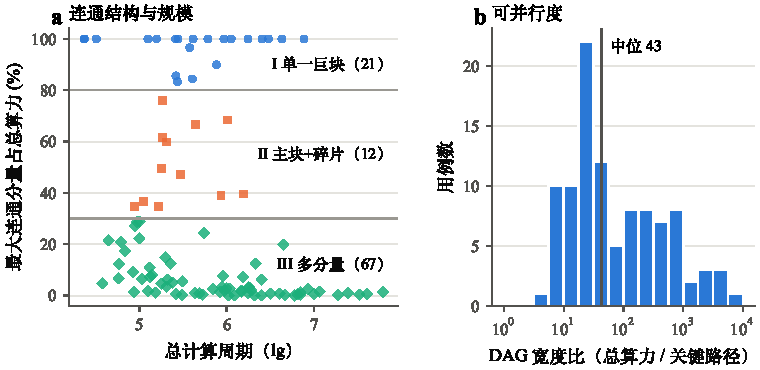
\includegraphics[width=\textwidth]{dataset_profile}
  \caption{测试集结构。(a) 最大弱连通分量的计算量占比 $\eta$ 与类别划分；(b) 宽度比 $\omega$ 的分布}
  \label{fig:dataset}
\end{figure}

\subsubsection{评价口径与性能参照}\label{sec:refs}

按题目定义，$k$ 核加速比为
\begin{equation}
  \rho_k=\frac{M_1^{\mathrm{sc}}}{M_k},\qquad \rho_1\equiv 1,
  \label{eq:speedup}
\end{equation}
其中 $M_1^{\mathrm{sc}}$ 是把整张图作为一个 Task 交给核内调度器得到的 Makespan，平均加速比取 100 个用例的算术平均。这个基准本身包含可以避免的开销：整张大图作为一个 Task 时，L1/UB 放不下全部中间张量，核内调度器会插入大量换入换出，而切成子图后每个子图的工作集变小，换出也随之减少。所以把图切开即使只用一个核也可能更快，$\rho_k>k$ 的超线性情形会出现。另外，题目附带的示例生成器 \texttt{stub\_multicore\_cut\_and\_schedule.py} 只生成格式合法的随机方案，以 case\_010 为例，它的 4 核方案 Makespan 为 88{,}416，比单核基准 86{,}969 还慢。用它作对照会高估算法效果，本文的对照基线一律采用第~\ref{sec:lpt} 节的分量装箱（$\alpha=0.25$），称为朴素基线。

只报告加速比，看不出离可达水平还有多远。我们用三个逐步收紧的参照值来衡量。第一个是解析下界：任何 $k$ 核方案都要完成全部计算、走完关键路径，并至少搬运一遍图的输入与输出，因此
\begin{equation}
  \underline{M}_k^{\mathrm{an}}=\max\left\{L_{\mathrm{cp}},\ \frac{W_M}{k},\ \frac{W_V}{k},\ \frac{Q_{\min}}{B}\right\},
  \label{eq:lb-analytic}
\end{equation}
$Q_{\min}$ 为图输入张量与输出张量的字节数之和。四项分别对应四个必须满足的条件：关键路径上的操作只能依次执行，所以 Makespan 不小于 $L_{\mathrm{cp}}$；全部 Cube 计算要分给 $k$ 个核心的 Cube 单元完成，负载最均衡时每个核心也要承担 $W_M/k$，Vector 同理；图的输入至少读入一次、输出至少写出一次，这些字节共享带宽 $B$，至少需要 $Q_{\min}/B$ 周期。Makespan 不小于其中任何一项，因而不小于它们的最大值。在忽略同步与换出的意义下，它是 Makespan 的下界，1 核时对应的平均加速比已达 \V{lb_k1_speedup_mean}，这也印证了单核基准中换出开销之大。第二个是零通信表调度：在 $D$ 上为每个核心设四条流水线，操作在前驱全部完成且对应流水线空闲时尽早开始，通信代价置零，所得 Makespan 记为 $M_k^0$，理想并行效率为
\begin{equation}
  \varepsilon_k=\frac{M_1^{0}}{k\,M_k^{0}}.
  \label{eq:ideal-eff}
\end{equation}
若依赖不构成任何限制，$k$ 核可以把单核的工作完全平分，$M_k^0=M_1^0/k$，效率为 1；依赖使部分核心在等待前驱时空闲，$M_k^0$ 大于 $M_1^0/k$，效率随之小于 1。所以 $\varepsilon_k$ 衡量的是依赖结构本身造成的并行损失。4 核时 $\varepsilon_4$ 的均值为 \V{ideal_k4_eff_mean}，只有 \V{ideal_k4_eff_lt50} 个用例低于 50\%，说明依赖结构本身几乎不限制并行，限制并行的是通信与同步。

第三个是含同步代价的可达参考。在同一表调度中加入固定的跨核延迟 $\delta$：操作 $v$ 放在核心 $n$ 上的最早开始时刻为
\begin{equation}
  \mathrm{EST}(v,n)=\max\Big\{\,\mathrm{avail}\big(n,\pi(v)\big),\ \max_{(u,v)\in A}\big(f_u+\delta_{un}\big)\Big\},\qquad
  \delta_{un}=\begin{cases}\delta, & \core(u)\ne n,\\ 0, & \core(u)=n,\end{cases}
  \label{eq:est-sync}
\end{equation}
其中 $\mathrm{avail}(n,p)$ 为核心 $n$ 上流水线 $p$ 的空闲时刻。$v$ 能开始，需要它所在的流水线已经空闲，并且所有前驱的结果都已可用：同核前驱完成即可用，跨核前驱还要再等 $\delta$ 周期，两者取最大就是最早开始时刻。就绪操作按自底向上关键路径长度降序处理，每个操作贪心地放到使 $\mathrm{EST}(v,n)+c_v$ 最小的核心；场景 A 取 $\delta=\delta_{\mathrm{cross}}$，场景 B 取 $\delta=\delta_B$。所得 Makespan 记为 $M_k^{\delta}$，本文结果对它的达成率定义为
\begin{equation}
  \mathrm{ach}_k=\frac{M_k^{\delta}}{M_k},
  \label{eq:achieve}
\end{equation}
它等于可达参考加速比 $M_1^{\mathrm{sc}}/M_k^{\delta}$ 与本文加速比 $M_1^{\mathrm{sc}}/M_k$ 之比，分子分母中的 $M_1^{\mathrm{sc}}$ 相互抵消，所以与单核基准无关。这一参照仍然忽略 DDR 争用和缓存换出，但计入了对小图影响最大的固定同步延迟。它是贪心结果，不是严格上界，实测结果可能超过它。三个参照值的平均加速比见表~\ref{tab:refs}，在各核数下依次递减，与逐步加入约束的构造一致。解析下界含搬运项而表调度不含，个别以搬运为主的用例上两者大小可能相反，这里的递减只就均值而言。从零通信到含同步，4 核平均加速比从 \V{p1_k4_ideal0_speedup_mean} 降到 \V{p1_k4_ref_speedup_mean}（场景 A），差的正是固定同步延迟的代价；对理想 Makespan 只有几千周期的小图，十几条跨核依赖链就能吃掉大部分并行收益。

\begin{table}[H]
\centering
\caption{性能参照的平均加速比（100 个用例）}
\label{tab:refs}
\renewcommand\arraystretch{1.15}
\begin{tabular}{lcccc}
\toprule
参照 & 2 核 & 3 核 & 4 核 & 5 核 \\
\midrule
解析下界，式 \eqref{eq:lb-analytic} & \V{lb_k2_speedup_mean} & \V{lb_k3_speedup_mean} & \V{lb_k4_speedup_mean} & \V{lb_k5_speedup_mean} \\
零通信表调度 & \V{p1_k2_ideal0_speedup_mean} & \V{p1_k3_ideal0_speedup_mean} & \V{p1_k4_ideal0_speedup_mean} & \V{p1_k5_ideal0_speedup_mean} \\
含同步可达参考，场景 A（$\delta=1000$） & \V{p1_k2_ref_speedup_mean} & \V{p1_k3_ref_speedup_mean} & \V{p1_k4_ref_speedup_mean} & \V{p1_k5_ref_speedup_mean} \\
含同步可达参考，场景 B（$\delta=500$） & \V{p2_k2_ref_speedup_mean} & \V{p2_k3_ref_speedup_mean} & \V{p2_k4_ref_speedup_mean} & \V{p2_k5_ref_speedup_mean} \\
\bottomrule
\end{tabular}
\end{table}

\subsection{问题一求解思路}

场景 A 中每个子图是一个独立 Task。评估程序为每个 Task 重建一张局部计算图：Task 读到但自己不生产的张量，在开头插入一次 COPY\_IN；Task 生产、且被别的 Task 使用或本身是图输出的张量，在结尾插入一次 COPY\_OUT。Task 之间不保留任何核内数据，两个 Task 即使在同一核心上相邻执行也是如此。Task 的激活受两类约束：同核前一个 Task 结束后至少等 $\delta_{\mathrm{same}}=100$ 周期，每个跨核前驱 Task 结束后至少等 $\delta_{\mathrm{cross}}=1000$ 周期。图~\ref{fig:sceneAB}(a) 以三个子图为例画出了这些规则，(b) 为第~\ref{sec:p2-model} 节要用到的场景 B。

\begin{figure}[H]
  \centering
  % 场景 A / B 的 Task 组织与边界搬运对比（3 个子图：s1、s2 在核 0，s3 在核 1；依赖 s1→s2、s1→s3）
\begin{tikzpicture}[x=1mm,y=1mm]
\tikzset{
  sgb/.style={pbox=cB, minimum width=11mm, minimum height=7mm, font=\footnotesize},
  cin/.style={draw=cO, fill=cOL, minimum width=3.2mm, minimum height=7mm, inner sep=0pt, font=\tiny, line width=0.5pt},
  task/.style={draw=ink2, dashed, rounded corners=2pt, inner sep=1.4mm, line width=0.5pt},
  ddr/.style={draw=cG, fill=cGL, minimum height=4mm, font=\scriptsize, text=ink2},
  lab/.style={font=\footnotesize\bfseries, text=ink2, anchor=east},
}
% ======================= (a) 场景 A =======================
\node[font=\small\bfseries, anchor=west] at (-10,25) {(a) 场景 A：每个子图一个 Task};
\node[lab] at (-1,10) {核 0};
\node[lab] at (-1,-10) {核 1};
\node[ddr, minimum width=62mm, anchor=west] (dA) at (0,0) {DDR};
\node[cin] (a1i) at (2,10) {I};
\node[sgb, right=0pt of a1i] (a1) {$s_1$};
\node[cin, right=0pt of a1] (a1o) {O};
\node[task, fit=(a1i)(a1o)] (t1) {};
\node[cin] (a2i) at (36,10) {I};
\node[sgb, right=0pt of a2i] (a2) {$s_2$};
\node[cin, right=0pt of a2] (a2o) {O};
\node[task, fit=(a2i)(a2o)] (t2) {};
\node[cin] (a3i) at (36,-10) {I};
\node[sgb, right=0pt of a3i] (a3) {$s_3$};
\node[cin, right=0pt of a3] (a3o) {O};
\node[task, fit=(a3i)(a3o)] {};
\draw[parrO] (a1o.south) -- ++(0,-7.5) -| (a2i.south);
\draw[parrO] (a1o.south) ++(0,-7.5) -| (a3i.north);
\draw[decorate, decoration={brace, amplitude=2pt}, draw=ink2] ($(t1.north east)+(0.5,1)$) -- node[above=2pt, pnote]{同核等待 $\ge 100$} ($(t2.north west)+(-0.5,1)$);
\node[pnote, text=cO, anchor=east] at ($(a3i.west)+(-3,0)$) {跨核等待 $\ge 1000$};
\node[pnote, anchor=north, text width=64mm, align=left] at (31,-17)
  {同核的 $s_1\to s_2$ 也要写回 DDR 再读入；\\每个 Task 结束都清空核内缓存};
% ======================= (b) 场景 B =======================
\begin{scope}[xshift=76mm]
\node[font=\small\bfseries, anchor=west] at (-10,25) {(b) 场景 B：每核一个 Task};
\node[lab] at (-1,10) {核 0};
\node[lab] at (-1,-10) {核 1};
\node[ddr, minimum width=62mm, anchor=west] (dB) at (0,0) {DDR};
\node[sgb] (b1) at (8,10) {$s_1$};
\node[cin, right=0pt of b1] (b1o) {O};
\node[sgb, right=12mm of b1o] (b2) {$s_2$};
\node[task, fit=(b1)(b1o)(b2)] {};
\draw[parrB] (b1.north) to[bend left=28] node[above, pnote]{L1/UB 驻留} (b2.north);
\node[cin] (b3i) at (36,-10) {I};
\node[sgb, right=0pt of b3i] (b3) {$s_3$};
\node[task, fit=(b3i)(b3)] {};
\draw[parrO] (b1o.south) -- ++(0,-7.5) -| (b3i.north);
\node[pnote, text=cO, anchor=east] at ($(b3i.west)+(-3,0)$) {同步 $+500$};
\node[pnote, anchor=north, text width=62mm, align=left] at (31,-17)
  {同核的 $s_1\to s_2$ 直接复用核内缓存，不产生搬运；\\只有跨核的 $s_1\to s_3$ 经 DDR，并等待 500 周期};
\end{scope}
\end{tikzpicture}

  \caption{场景 A 与场景 B 的 Task 组织与边界搬运（$s_1$、$s_2$ 在核 0，$s_3$ 在核 1；I、O 分别为评估程序插入的 COPY\_IN、COPY\_OUT）}
  \label{fig:sceneAB}
\end{figure}

由这些规则，场景 A 方案的时间代价有四个来源：某个核心计算量明显偏多造成的负载不均衡；跨子图张量写回 DDR 再读入的边界搬运，它还要和其他核心争用 60 bytes/cycle 的总带宽；沿依赖链每经过一次子图边界就要付出的 100 或 1000 周期激活等待；以及子图过大、核内缓存装不下时插入的换入换出。前三项中，后两项随依赖路径上的子图边界增加而变重，而负载均衡和换出又要求子图不能太少、太大。求解思路据此分三步。第一步建立切图与调度的优化模型，把边界搬运和路径上累积的等待写成显式表达式，从中得到“少在依赖链上切分、少跨核”的原则。第二步针对不同结构设计三种构造算法：多分量图按分量装箱，单一巨块图按层级切带，汇聚链结构用通信感知的表调度决定分核、再按换核次数组成子图；三种算法都由构造保证商图无环。第三步对每个（用例，核数）组合在参数网格上生成候选，由官方评估程序选优，再做成组合并、局部搜索和核数补齐三种后处理。整个过程如图~\ref{fig:ladder-p1} 所示，每一步都针对前一步在数据上暴露的不足。

\begin{figure}[H]
  \centering
  % 问题一的求解步骤（5 核平均加速比，数字取自 numbers.tex）
\begin{tikzpicture}[x=1mm,y=1mm]
\def\dx{30}\def\dy{10}
\tikzset{st/.style={pbox=#1, text width=24mm, minimum height=14mm, anchor=south west, font=\footnotesize}}
\node[st=cG] (s0) at (0,0)        {分量装箱\\[1pt]\textbf{\V{p1_k5_lpt_mean}}};
\node[st=cB] (s1) at (\dx,\dy)    {+ 层带划分\\[1pt]\textbf{\V{p1_k5_lptband_mean}}};
\node[st=cB] (s2) at (2*\dx,2*\dy){+ 相位构造\\[1pt]\textbf{\V{ladder_p1_k5_sweep}}};
\node[st=cO] (s3) at (3*\dx,3*\dy){+ 成组合并\\[1pt]\textbf{\V{ladder_p1_k5_coarsen}}};
\node[st=cO, line width=1pt] (s4) at (4*\dx,4*\dy){+ 局部搜索\\+ 核数补齐\\[1pt]\textbf{\V{ladder_p1_k5_monotone}}};
\foreach \i/\j in {0/1,1/2,2/3,3/4} \draw[parrO] (s\i.north) |- (s\j.west);
\tikzset{why/.style={pnote, text=cO, anchor=north, text width=25mm, font=\scriptsize}}
\node[why] at ($(s1.south)+(0,-1)$) {I 类 4 核仅 \V{p1_k4_famI_naive_mean}};
\node[why] at ($(s2.south)+(0,-1)$) {汇聚链跨核依赖多};
\node[why] at ($(s3.south)+(0,-1)$) {同核 Task 过碎};
\node[why] at ($(s4.south)+(0,-1)$) {部分用例多核反慢};
\node[pnote, anchor=north, text width=25mm, font=\scriptsize] at ($(s0.south)+(0,-1)$) {$\alpha=0.25$：\V{p1_k5_naive_mean}};
\draw[-{Stealth[length=2mm]}, line width=0.7pt, draw=ink2] (-3,-12) -- (148,-12) node[pnote, anchor=north east] {评估次数 $\rightarrow$};
\end{tikzpicture}

  \caption{问题一的求解步骤与 5 核平均加速比。框下文字为引入该步的原因，首框下为朴素参数的结果}
  \label{fig:ladder-p1}
\end{figure}

\subsection{问题一模型建立}\label{sec:p1-model}

\subsubsection{决策变量与合法性约束}

给定核数 $k$，决策变量为：$x_{vs}\in\{0,1\}$ 表示操作 $v\in\Oe$ 属于子图 $s$，$y_{sn}\in\{0,1\}$ 表示子图 $s$ 分配到核心 $n$，$z_{ss'}\in\{0,1\}$ 表示同核的子图 $s$ 排在 $s'$ 之前。每个可分配操作恰好属于一个子图，每个非空子图恰好分到一个核心：
\begin{equation}
  \sum_{s\in S} x_{vs}=1,\ \ \forall v\in \Oe;\qquad
  \sum_{n=1}^{k} y_{sn}=1,\ \ \forall s\in S .
  \label{eq:assign}
\end{equation}
子图之间的依赖定义为 $s\to s' \iff \exists (u,v)\in A:\ \sg(u)=s,\ \sg(v)=s',\ s\ne s'$，题目要求由此得到的子图依赖图（下称商图）无环。引入子图拓扑秩 $r_s\in\mathbb{Z}_{\ge 0}$，无环约束可以线性化为
\begin{equation}
  r_{s'}\ \ge\ r_s+1-|S|\,(2-x_{us}-x_{vs'}),\qquad \forall (u,v)\in A,\ \ s\ne s' .
  \label{eq:acyclic}
\end{equation}
当 $u\in s$、$v\in s'$ 时右端为 $r_s+1$，否则约束自动满足。存在满足式 \eqref{eq:acyclic} 的 $r$ 与商图无环等价：无环时取任一拓扑序中的位置作为 $r$ 即可；若有环，沿环把式 \eqref{eq:acyclic} 相加得到 $0\ge$ 环长，矛盾。同核子图的执行顺序还必须与依赖相容：
\begin{equation}
  z_{ss'}+z_{s's}\ \ge\ y_{sn}+y_{s'n}-1,\qquad z_{ss'}\ \ge\ a_{ss'}\,(y_{sn}+y_{s'n}-1),\qquad \forall n,\ s\ne s' ,
  \label{eq:order}
\end{equation}
其中 $a_{ss'}\in\{0,1\}$ 表示 $s\to s'$ 是否成立。当 $s$、$s'$ 都在核心 $n$ 上时 $y_{sn}+y_{s'n}-1=1$，第一式要求 $z_{ss'}$ 与 $z_{s's}$ 至少一个为 1，即两个子图必须排出先后；若再有 $s\to s'$，第二式强制 $z_{ss'}=1$，即被依赖的子图排在前面。两者不同核时右端不大于 0，约束自动满足。

\subsubsection{边界搬运量}

记 $\sg(X)=\{\sg(v):v\in X\}$。按评估程序的插入规则，张量 $t$ 在场景 A 下被读入、写出的次数分别为
\begin{equation}
  n^{\mathrm{in}}_t=\big|\sg(U_t)\setminus \sg(P_t)\big|,\qquad
  n^{\mathrm{out}}_t=\big|\{\,s\in \sg(P_t):\ t\in T_{\mathrm{out}}\ \text{或}\ \sg(U_t)\setminus\{s\}\ne\varnothing\,\}\big| ,
  \label{eq:copies-A}
\end{equation}
切图新增的搬运字节数为
\begin{equation}
  Q_A=\sum_{t\in T} s_t\big(n^{\mathrm{in}}_t+n^{\mathrm{out}}_t\big)-Q_{\mathrm{orig}}.
  \label{eq:QA}
\end{equation}
式 \eqref{eq:QA} 的求和逐张量统计切图后的全部 COPY 字节，减去原图已有的 COPY 字节，剩下的就是切图新增的部分。总额外搬运量还要加上核内换入换出的字节数 $Q^{\mathrm{sp}}$，它由核内调度器决定，写不成方案的显式函数。式 \eqref{eq:copies-A} 说明，中间张量只要跨出生产它的子图，就至少多一次写出和一次读入；图输入张量被 $m$ 个子图使用时要从 DDR 读 $m$ 次，比原图多读 $m-1$ 次，这就是题目所说的重复读取代价。

\subsubsection{时间模型与目标}

对子图 $s$，记其 Task 的激活、结束时刻为 $b_s,e_s$，$s^-$ 为同核上排在 $s$ 之前的子图。由场景 A 的激活规则，
\begin{equation}
  b_s\ \ge\ e_{s^-}+\delta_{\mathrm{same}},\qquad
  b_s\ \ge\ e_{s'}+\delta_{\mathrm{cross}},\ \ \forall s'\to s,\ \core(s')\ne\core(s).
  \label{eq:activate}
\end{equation}
第一式来自同核串行执行：前一个 Task 结束后要经过 $\delta_{\mathrm{same}}$ 的切换才能激活下一个；第二式来自跨核依赖：$s$ 用到的数据要等跨核前驱 $s'$ 结束并经过 $\delta_{\mathrm{cross}}$ 才可用。$b_s$ 必须同时满足这两类约束。Task 内部 Cube、Vector 与搬运流水线可以并行，其持续时间至少为
\begin{equation}
  e_s-b_s\ \ge\ d_s:=\max\Big\{w_M(s),\ w_V(s),\ \frac{Q^{\mathrm{io}}_s}{B}\Big\},
  \label{eq:task-dur}
\end{equation}
$Q^{\mathrm{io}}_s$ 为该 Task 的边界搬运字节数。三项分别是 Cube 流水线、Vector 流水线和搬运流水线各自至少要忙碌的时间：同一条流水线上的操作只能依次执行，而搬运即使独占带宽 $B$ 也需要 $Q^{\mathrm{io}}_s/B$ 周期，Task 不可能比其中最忙的一条更早结束。综合以上约束，问题一的模型为
\begin{equation}
\begin{aligned}
  \min\quad & M_k=\max_{s\in S} e_s\\
  \text{s.t.}\quad & \text{划分与分核约束 \eqref{eq:assign}，无环约束 \eqref{eq:acyclic}，同核顺序约束 \eqref{eq:order}},\\
  & \text{激活约束 \eqref{eq:activate}，持续时间约束 \eqref{eq:task-dur}},\\
  & x_{vs},\,y_{sn},\,z_{ss'}\in\{0,1\},\quad r_s\in\mathbb{Z}_{\ge 0},
\end{aligned}
  \label{eq:obj-p1}
\end{equation}
以 $Q_A+Q^{\mathrm{sp}}$ 为次要目标。真实的 $e_s$ 还受 DDR 带宽争用和核内换出影响，式 \eqref{eq:task-dur} 只是下界，所以式 \eqref{eq:obj-p1} 是真实问题的松弛。它虽然不能直接求解，但能推出两个决定算法设计的结论。第一个结论刻画了依赖路径上的代价。

\begin{proposition}\label{prop:path}
对商图中任意一条路径 $s_1\to s_2\to\cdots\to s_m$，若其中相邻子图在不同核心上的次数为 $h$，则
\begin{equation}
  M_k\ \ge\ \sum_{i=1}^{m} d_{s_i}+h\,\delta_{\mathrm{cross}}+(m-1-h)\,\delta_{\mathrm{same}} .
  \label{eq:path-bound}
\end{equation}
\end{proposition}
\begin{proof}
跨核时由式 \eqref{eq:activate} 有 $b_{s_{i+1}}\ge e_{s_i}+\delta_{\mathrm{cross}}$；同核时由式 \eqref{eq:order}，$s_i$ 排在 $s_{i+1}$ 之前，$s_{i+1}$ 的同核前驱结束不早于 $e_{s_i}$，故 $b_{s_{i+1}}\ge e_{s_i}+\delta_{\mathrm{same}}$。再由式 \eqref{eq:task-dur} 有 $e_{s_i}\ge b_{s_i}+d_{s_i}$，沿路径累加即得。
\end{proof}

式 \eqref{eq:path-bound} 表明，场景 A 的固定延迟沿商图路径线性累积，代价取决于路径上的子图边界数，而不是子图总数：把互不相连的分量切成很多子图，并不会拉长任何一条路径。4--5 核的小图理想 Makespan 只有数千周期，路径上出现三四次跨核，延迟就会超过计算本身。所以好的场景 A 方案要让依赖链尽量留在同一子图、同一核心内，只在能换来并行度的地方切开。第二个结论说明精确求解不可行。

\begin{proposition}\label{prop:np}
式 \eqref{eq:obj-p1} 所定义的问题是强 NP 难的。
\end{proposition}
\begin{proof}
取没有边、每个操作只有 Cube 计算的特殊实例。此时任意划分都合法，Makespan 等于最大的核心负载，问题退化为同构并行机调度 $P\|C_{\max}$；$k$ 作为输入时，它可由 3-划分问题归约，是强 NP 难的\cite{garey1978strong}。特殊情形已强 NP 难，一般情形亦然。
\end{proof}

带无环约束的图划分本身也是 NP 难的\cite{herrmann2019acyclic}，而测试用例最大有 35{,}705 个操作。更重要的是，式 \eqref{eq:obj-p1} 只是松弛，它的最优解不一定是评估程序下的最优解。因此我们用模型指导算法设计：由命题~\ref{prop:path} 得到少在依赖链上切分、少跨核的原则，由负载项得到按计算量装箱的原则，最终由官方评估程序裁决。

\subsection{问题一模型求解与结果分析}

\subsubsection{算法描述}

\label{sec:lpt}第一种构造是分量装箱与拓扑区间切分，思路是把互不相连的部分分给不同核心（算法~\ref{alg:lpt}）。先求 $D$ 的弱连通分量，对每个分量沿生产者—消费者链做深度优先风格的拓扑排序，使相邻操作在序列中也相邻，拼接得到全局序 $\tau$。计算量超过上限 $\bar w$ 的分量沿 $\tau$ 顺序累加，超过 $\bar w$ 就切开，记为 $\mathrm{Split}_\tau(C,\bar w)$。所有区间按 $\widehat w$ 降序，依次放到放入后二维负载最小的核心，即最长处理时间优先（LPT）规则。$\alpha$ 越大，$\bar w$ 越小，负载越均衡，但被切断的依赖越多，式 \eqref{eq:path-bound} 中的路径代价也越大，两者此消彼长，没有对所有用例都合适的取值。连通分量与拓扑排序为 $O(|\Oe|+|A|)$，装箱为 $O(m\log m+mk)$，$m$ 为区间数。这一方法在多分量图上效果好，但在单一巨块图上，整张图只有一个分量，$\alpha$ 较小时不被切开，全部工作落在一个核上；调大 $\alpha$ 把它切成区间，$\tau$ 中相邻区间之间依赖很密，跨核后几乎串行。

\begin{algorithm}[H]
\caption{分量装箱与拓扑区间切分 $\mathrm{LPT}(D,k,\alpha)$}\label{alg:lpt}
\begin{algorithmic}[1]
\Require $D=(\Oe,A)$，$k$，$\alpha$
\Ensure $\sg$，$\{\Pi_n\}_{n=1}^{k}$
\State $\{C_1,\dots,C_q\}\gets \mathrm{WCC}(D)$；$\tau\gets \mathrm{DFSTopo}(C_1)\,\|\cdots\|\,\mathrm{DFSTopo}(C_q)$
\State $\bar w\gets \max(W_M,W_V)/(k\alpha)$；$\mathcal{I}\gets\varnothing$
\For{$j=1,\dots,q$}
  \If{$\widehat w(C_j)\le \bar w$} $\mathcal{I}\gets\mathcal{I}\cup\{C_j\}$
  \Else\ $\mathcal{I}\gets\mathcal{I}\cup \mathrm{Split}_\tau(C_j,\bar w)$
  \EndIf
\EndFor
\State $L_M^n\gets 0,\ L_V^n\gets 0,\ \forall n$
\For{$I\in\mathcal{I}$，按 $\widehat w(I)$ 降序}
  \State $n^*\gets\argmin_n \max\{L_M^n+w_M(I),\ L_V^n+w_V(I)\}$
  \State $\core(I)\gets n^*$；$L_M^{n^*}\gets L_M^{n^*}+w_M(I)$；$L_V^{n^*}\gets L_V^{n^*}+w_V(I)$
\EndFor
\State $\sg(v)\gets I\ni v$；$\Pi_n\gets\{I:\core(I)=n\}$ 按 $\min_{v\in I}\tau(v)$ 升序
\end{algorithmic}
\end{algorithm}

第二种构造是层带 $\times$ 核划分，针对单一巨块图。这类图只有一个分量，但 I 类宽度比中位数仍有 \V{famI_width_median}，同一时刻有十几路计算可以并行，只是互相交织。层带划分（算法~\ref{alg:band}）按从源点起的最长路径层级 $\ell(v)$ 把操作分层，再按累计计算量把层级切成 $W$ 个连续的层带。同一层带内的操作大多互不依赖，可以分到不同核心；带内仍有直接依赖的操作用并查集并成原子组，同组必须同核。每个层带内对原子组做 LPT 装箱，每个（层带，核心）组合成为一个子图。层级计算与并查集为 $O(|\Oe|+|A|)$，各带装箱合计 $O(|\Oe|\log|\Oe|+|\Oe|k)$。它让单一巨块图可以并行，但按层级而不是按分量切，会把多分量图中本来互不相干的分量也切碎。

\begin{algorithm}[H]
\caption{层带 $\times$ 核划分 $\mathrm{BAND}(D,k,W)$}\label{alg:band}
\begin{algorithmic}[1]
\Require $D=(\Oe,A)$，$k$，$W$
\Ensure $\sg$，$\{\Pi_n\}_{n=1}^{k}$
\State 计算 $\ell(v),\ \forall v\in\Oe$；把层级切成连续层带 $\mathcal{B}_1,\dots,\mathcal{B}_W$，使 $\sum_{v\in\mathcal{B}_b}c_v$ 近似相等
\State $\Pi_n\gets\varnothing,\ \forall n$
\For{$b=1,\dots,W$}
  \State $\mathcal{G}_b\gets \mathrm{UnionFind}\big(\mathcal{B}_b,\ \{(u,v)\in A:u,v\in\mathcal{B}_b\}\big)$
  \State 对 $\mathcal{G}_b$ 按算法~\ref{alg:lpt} 的 LPT 规则装箱，得 $\core(g),\ g\in\mathcal{G}_b$
  \For{$n=1,\dots,k$}
    \State $s_{b,n}\gets\bigcup\{g\in\mathcal{G}_b:\core(g)=n\}$；若 $s_{b,n}\ne\varnothing$，$\Pi_n\gets\Pi_n\oplus s_{b,n}$
  \EndFor
\EndFor
\end{algorithmic}
\end{algorithm}

第三种构造是通信感知表调度与相位构造。它针对的结构介于前两类之间：若干条并行链最后汇聚在一起。前两种方法只按计算量切分，不考虑切断一条依赖要付出多少代价。算法~\ref{alg:phase} 分两步。第一步在操作粒度上做与 HEFT\cite{topcuoglu2002performance} 类似的表调度，决定每个操作放在哪个核心：就绪操作按自底向上关键路径长度 $\mathrm{bl}(v)$ 降序处理，操作 $v$ 放在核心 $n$ 的估计完成时刻为
\begin{equation}
  F(v,n)=\max\Big\{\mathrm{avail}\big(n,\pi(v)\big),\ \max_{(u,v)\in A}\big(f_u+g_{un}\big)\Big\}+c_v ,\qquad
  g_{un}=\begin{cases}\lambda+s_{\mathrm{out}}(u)/B, & \core(u)\ne n,\\ 0, & \core(u)=n,\end{cases}
  \label{eq:phase-est}
\end{equation}
取使 $F$ 最小的核心，$s_{\mathrm{out}}(u)$ 为 $u$ 的输出字节数。式 \eqref{eq:phase-est} 的推理与式 \eqref{eq:est-sync} 相同：$v$ 要等流水线空闲和全部前驱结果可用，跨核前驱的结果要额外付出惩罚 $\lambda$ 和把输出张量按带宽 $B$ 搬过去的时间，再加上自身周期 $c_v$ 就是完成时刻。与式 \eqref{eq:est-sync} 不同，跨核惩罚 $\lambda$ 不必等于真实的同步延迟：取得越大，算法越不愿意跨核，子图越少。第二步把操作级的分核结果组成子图。定义相位
\begin{equation}
  \phi(v)=\max_{(u,v)\in A}\big\{\phi(u)+\chi_{uv}\big\},\qquad
  \chi_{uv}=\begin{cases}1, & \core(u)\ne\core(v),\\ 0, & \core(u)=\core(v),\end{cases}\qquad \phi(v)=0\ \ \text{若 $v$ 无前驱},
  \label{eq:phase}
\end{equation}
即从源点到 $v$ 的路径上最多换过几次核。每个（核心，相位）组合成为一个子图，各核按相位递增排列。图~\ref{fig:phase-ex} 是一个 7 个操作、2 个核心的例子：$e$ 的前驱 $d$ 在另一个核心上，相位加 1；$g$ 又从 $e$ 跨核，相位再加 1，最终形成 4 个子图。沿任意操作路径，相位的增量恰好是换核次数，所以相位构造方案的换核深度 $h$ 就等于 $\max_v\phi(v)$，而 $\lambda$ 直接压低了它。算法复杂度为 $O(k(|\Oe|+|A|)+|\Oe|\log|\Oe|)$。三种构造都不需要事后检查合法性，因为它们都给子图一个随依赖严格递增的编号，这一点由下面的命题~\ref{prop:acyclic} 保证。

\begin{figure}[H]
  \centering
  % 相位构造示例：7 个操作，2 核；蓝 = 核 0，橙 = 核 1；节点旁为相位 φ；虚线框为最终子图
\begin{tikzpicture}[x=1mm,y=1mm]
\tikzset{lbl/.style={font=\scriptsize, text=ink2}, grp/.style={pgroup, inner sep=2.2mm},
         opA/.append style={minimum size=9mm, align=center}, opB/.append style={minimum size=9mm, align=center}}
\newcommand{\ph}[2]{$#1$\\[-2pt]{\tiny$\phi{=}#2$}}
\node[font=\bfseries\small] at (-8,9) {a};
\node[opA] (a) at (0,0) {\ph{a}{0}};
\node[opB] (b) at (0,-18) {\ph{b}{0}};
\node[opA] (c) at (16,0) {\ph{c}{0}};
\node[opB] (d) at (16,-18) {\ph{d}{0}};
\node[opA] (e) at (34,0) {\ph{e}{1}};
\node[opA] (f) at (50,0) {\ph{f}{1}};
\node[opB] (g) at (50,-18) {\ph{g}{2}};
\draw[parr] (a) -- (c); \draw[parr] (b) -- (d); \draw[parr] (c) -- (e); \draw[parr] (e) -- (f);
\draw[parrO] (d) -- node[pnote, left, pos=0.5]{$+1$} (e);
\draw[parrO] (e) -- node[pnote, right, pos=0.5]{$+1$} (g);
\begin{scope}[on background layer]
\node[grp, fit=(a)(c)] (S1) {}; \node[grp, fit=(b)(d)] (S2) {};
\node[grp, fit=(e)(f)] (S3) {}; \node[grp, fit=(g)] (S4) {};
\end{scope}
\node[pnote, anchor=south west] at (S1.north west) {$S_1{=}(0,0)$};
\node[pnote, anchor=north west] at (S2.south west) {$S_2{=}(1,0)$};
\node[pnote, anchor=south east] at (S3.north east) {$S_3{=}(0,1)$};
\node[pnote, anchor=north east] at (S4.south east) {$S_4{=}(1,2)$};
% 右侧：商图与各核序列
\begin{scope}[xshift=76mm, yshift=-8mm]
\node[font=\bfseries\small, anchor=west] at (-8,15) {b};
\node[pbox=cB, minimum width=10mm] (q1) at (0,6) {$S_1$};
\node[pbox=cO, minimum width=10mm] (q2) at (0,-6) {$S_2$};
\node[pbox=cB, minimum width=10mm] (q3) at (16,6) {$S_3$};
\node[pbox=cO, minimum width=10mm] (q4) at (32,-6) {$S_4$};
\draw[parr] (q1) -- (q3); \draw[parrO] (q2) -- (q3); \draw[parrO] (q3) -- (q4);
\node[pnote, anchor=north west, align=left] at (-6,-13) {$\Pi_0=(S_1,S_3)$，\ $\Pi_1=(S_2,S_4)$};
\end{scope}
\end{tikzpicture}

  \caption{相位构造示例（蓝色为核 0，橙色为核 1，节点内为相位 $\phi$）。(a) 操作级分核结果，虚线框为形成的子图；(b) 商图与各核子图序列}
  \label{fig:phase-ex}
\end{figure}

\begin{algorithm}[H]
\caption{通信感知表调度与相位构造 $\mathrm{PHASE}(D,k,\lambda)$}\label{alg:phase}
\begin{algorithmic}[1]
\Require $D=(\Oe,A)$，$k$，$\lambda$
\Ensure $\sg$，$\{\Pi_n\}_{n=1}^{k}$
\State 计算 $\mathrm{bl}(v),\ \forall v$；$\mathcal{R}\gets\{v:\ \nexists (u,v)\in A\}$
\While{$\mathcal{R}\ne\varnothing$}
  \State $v\gets\argmax_{u\in\mathcal{R}}\mathrm{bl}(u)$；$\mathcal{R}\gets\mathcal{R}\setminus\{v\}$
  \State $\core(v)\gets\argmin_n F(v,n)$；$f_v\gets F(v,\core(v))$；更新 $\mathrm{avail}(\core(v),\pi(v))$
  \State $\mathcal{R}\gets\mathcal{R}\cup\{w:(v,w)\in A,\ w \text{ 的前驱均已调度}\}$
\EndWhile
\State 按拓扑序由式 \eqref{eq:phase} 计算 $\phi(v)$
\State $\sg(v)\gets(\core(v),\phi(v))$；$\Pi_n\gets\{\sg(v):\core(v)=n\}$ 按 $\phi$ 升序
\end{algorithmic}
\end{algorithm}


\begin{proposition}\label{prop:acyclic}
算法~\ref{alg:lpt}、\ref{alg:band}、\ref{alg:phase} 产生的商图均无环，且各核的子图顺序与依赖相容。层带划分下，商图任一路径最多经过 $W$ 个子图，从而换核深度 $h\le W-1$。
\end{proposition}
\begin{proof}
三种构造各给子图一个编号：算法~\ref{alg:lpt} 为区间起点在 $\tau$ 中的位置，算法~\ref{alg:band} 为层带号，算法~\ref{alg:phase} 为相位。只需证明对任意 $(u,v)\in A$，若 $\sg(u)\ne\sg(v)$，则 $\sg(u)$ 的编号严格小于 $\sg(v)$ 的编号，这样按编号排序就是商图的拓扑序，同核按编号排列也就与依赖相容。对算法~\ref{alg:lpt}，$\tau(u)<\tau(v)$，而区间互不相交且连续，所以 $u$ 所在区间整体位于 $v$ 所在区间之前。对算法~\ref{alg:band}，$\ell(u)<\ell(v)$，层带由连续层级组成，故 $u$ 的层带号不大于 $v$ 的；若相等，$u,v$ 由带内直接边相连，属同一原子组，必在同一子图。对算法~\ref{alg:phase}，由式 \eqref{eq:phase} 有 $\phi(v)\ge\phi(u)$，跨核时严格大于；若同核且不同子图，则相位不同，仍有 $\phi(v)>\phi(u)$。最后，层带划分下商图的每条边都严格增大层带号，而层带号只有 $W$ 个取值，故任一路径最多 $W$ 个子图。
\end{proof}

命题~\ref{prop:acyclic} 与命题~\ref{prop:path} 结合，说明层带数 $W$ 同时控制并行度和最坏情形下的路径代价 $(W-1)\delta_{\mathrm{cross}}$，场景 A 中后者代价高，应偏向较小的 $W$。表~\ref{tab:param} 的扫描结果与这一判断一致：问题一中固定 $W=16$ 的平均加速比高于 $W=256$ 和 $W=4096$。但 $W$ 也不能过小，层带太少时每个层带内操作过多，带内有直接依赖的操作被并成大的原子组，装箱就难以均衡，所以最终仍要逐用例选择 $W$。

\label{sec:post}三种构造算法各有擅长的结构，参数的合适取值也相差几个数量级。算法~\ref{alg:select} 对每个（用例，核数）组合生成候选集 $\mathcal{C}_{p,k}$，全部交给评估程序，取 $E_p$ 最小者，再做三种后处理。参数网格为：$\alpha\in\mathcal{A}=\{0.1,0.25,0.5,1,2,4,8\}$；$W\in\mathcal{W}=\{16,256,4096\}$，对 I、II 类共 33 个用例加密为 $\{16,32,64,128,256,512,1024,4096\}$；$\lambda\in\Lambda=\{2000,10^4,5\times10^4\}$，对同样 33 例加密为 $\{500,1000,2000,5000,10^4,2\times10^4,5\times10^4,10^5\}$。

成组合并把每个核心上相邻的 $w$ 个子图合为一个，不改变任何操作的核心。记 $\mathrm{pos}(s)$ 为子图 $s$ 在所在核心序列中的位置，宽度为 $w$ 的合并把 $s^n_i$ 映射到第 $\lceil i/w\rceil$ 组：
\begin{equation}
  \sg'(v)=g^{\core(v)}_{\lceil \mathrm{pos}(\sg(v))/w\rceil},
  \label{eq:coarsen}
\end{equation}
宽度取 $w\in\{2,4,\dots,128\}$，合并范围取全部核心、仅最后一个核心、除最后一个核心三种，共 21 个候选，记为 $\mathrm{Coarsen}(x,w,c)$。合并后同核顺序仍按原位置排列，只可能因为“从组内出发、经过别的核心、又回到组内”的依赖路径而成环，这类候选由评估程序的合法性检查剔除。场景 A 中，合并直接减少了 Task 数，式 \eqref{eq:path-bound} 中的同核切换次数和边界搬运随之减少。

局部搜索以候选方案 $x$ 为起点，邻域为
\begin{equation}
  \mathcal{N}(x)=\mathcal{N}_{\mathrm{move}}(x)\cup\mathcal{N}_{\mathrm{swap}}(x)\cup\mathcal{N}_{\mathrm{merge}}(x)\cup\mathcal{N}_{\mathrm{split}}(x),
  \label{eq:nbhd}
\end{equation}
四类动作分别是把一个子图移到另一个核心、交换两个核心上的子图、合并同核相邻的两个子图、把一个子图沿拓扑序切成两半。每步随机抽一个动作（合并的概率加倍），先用评估程序自带的合法性检查预筛，再做完整评估，仅当 $E_p(x')<E_p(x)$ 时接受，即纯爬山。核数补齐利用题目允许空核的规定：$k'$ 核方案补上 $k-k'$ 个空核，记为 $\mathrm{Pad}(x,k)$，就是合法的 $k$ 核方案；若某用例 $k'$ 核（$k'<k$）的结果优于 $k$ 核，就用补齐后的方案替换，使结果随核数单调不增。

\begin{algorithm}[H]
\caption{逐用例选优与后处理}\label{alg:select}
\begin{algorithmic}[1]
\Require $D$，$k$，$p$，$E_p$，局部搜索步数 $N_{\mathrm{LS}}$，已选方案 $x^*_{k'}\ (k'<k)$
\Ensure $x^*_k$
\State $\mathcal{C}_{p,k}\gets\{\mathrm{LPT}(D,k,\alpha)\}_{\alpha\in\mathcal{A}}\cup\{\mathrm{BAND}(D,k,W)\}_{W\in\mathcal{W}}\cup\{\mathrm{PHASE}(D,k,\lambda)\}_{\lambda\in\Lambda}$
\State $x\gets\argmin_{x'\in\mathcal{C}_{p,k}}E_p(x')$
\State $x\gets\argmin\big\{E_p(x'):\ x'\in\{x\}\cup\{\mathrm{Coarsen}(x,w,c)\}_{w,c},\ x' \text{ 合法}\big\}$
\For{$i=1,\dots,N_{\mathrm{LS}}$}
  \State 随机取 $x'\in\mathcal{N}(x)$；若 $x'$ 合法且 $E_p(x')<E_p(x)$，则 $x\gets x'$
\EndFor
\State $x^*_k\gets\argmin\big\{E_p(x'):\ x'\in\{x\}\cup\{\mathrm{Pad}(x^*_{k'},k)\}_{k'<k}\big\}$
\end{algorithmic}
\end{algorithm}

\subsubsection{求解分析}

扫描阶段共完成 \V{pf_evals} 次官方评估。表~\ref{tab:algo-p1} 对比了单一构造算法与逐用例选优（各算法已在自身参数网格上逐用例取最优）。任何单一算法都明显落后：5 核时最好的单一算法是分量装箱，平均 \V{p1_k5_lpt_mean}，逐用例选优为 \V{p1_k5_portfolio_mean}；获胜算法也很分散，5 核时分量装箱、层带划分、相位构造分别在 \V{p1_k5_algo_wins_lpt}、\V{p1_k5_algo_wins_band}、\V{p1_k5_algo_wins_phase} 个用例上胜出。图~\ref{fig:algocmp}(a) 画出了同样的对比，核数越多，单一算法与选优的差距越大。相位构造中 $\lambda$ 的作用尤其明显：case\_002 在 4 核下 $\lambda$ 从 2000 增至 50000，加速比从 2.17 升到 3.33。

\begin{table}[H]
\centering
\caption{问题一：单一构造算法与逐用例选优的平均加速比}
\label{tab:algo-p1}
\renewcommand\arraystretch{1.15}
\begin{tabular}{lcccc}
\toprule
方法 & 2 核 & 3 核 & 4 核 & 5 核 \\
\midrule
朴素基线（分量装箱，$\alpha=0.25$） & \V{p1_k2_naive_mean} & \V{p1_k3_naive_mean} & \V{p1_k4_naive_mean} & \V{p1_k5_naive_mean} \\
分量装箱 & \V{p1_k2_lpt_mean} & \V{p1_k3_lpt_mean} & \V{p1_k4_lpt_mean} & \V{p1_k5_lpt_mean} \\
层带划分 & \V{p1_k2_band_mean} & \V{p1_k3_band_mean} & \V{p1_k4_band_mean} & \V{p1_k5_band_mean} \\
相位构造 & \V{p1_k2_phase_mean} & \V{p1_k3_phase_mean} & \V{p1_k4_phase_mean} & \V{p1_k5_phase_mean} \\
逐用例选优 & \V{p1_k2_portfolio_mean} & \V{p1_k3_portfolio_mean} & \V{p1_k4_portfolio_mean} & \V{p1_k5_portfolio_mean} \\
加后处理（最终） & \V{p1_k2_final_mean} & \V{p1_k3_final_mean} & \V{p1_k4_final_mean} & \V{p1_k5_final_mean} \\
\bottomrule
\end{tabular}
\end{table}

\begin{figure}[H]
  \centering
  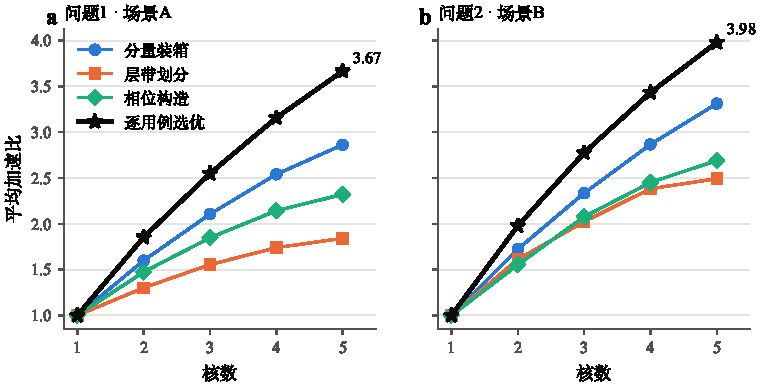
\includegraphics[width=\textwidth]{algo_compare}
  \caption{构造算法（各自在参数网格上逐用例取最优）与逐用例选优的平均加速比。(a) 问题一；(b) 问题二}
  \label{fig:algocmp}
\end{figure}

后处理中，第一轮成组合并在 \V{co1_p1_groups} 组（用例，核数）中改进了 \V{co1_p1_improved} 组，平均缩短 \V{co1_p1_mean_red_pct}，最多 \V{co1_p1_max_red_pct}；以第一轮结果为起点换用更细宽度的第二轮，\V{co2_groups} 组平均只再缩短 \V{co2_mean_red_pct}，这一方向已基本挖尽。局部搜索共运行 \V{ls_jobs_total} 个作业，每个作业的评估次数中位数 \V{ls_tries_median}、用时中位数 \V{ls_secs_median} 秒，问题一中起点可追溯的 \V{ls_p1_jobs} 个作业平均缩短 \V{ls_p1_mean_red_pct}，最多 \V{ls_p1_max_red_pct}。它的平均收益远小于换一种构造方式，我们保留它是因为在个别用例上没有替代：最终方案中问题一有 \V{source_mix_by_problem_1_localsearch} 组来自局部搜索。核数补齐在问题一中评估了 \V{mono_p1} 个补空核方案，重评后的 Makespan 与原少核方案逐个相同。补齐之后，每个用例的加速比都随核数单调不减，满足题目对 2--5 核稳定性的要求。

最终的平均加速比见图~\ref{fig:speedup}(a) 与表~\ref{tab:p1-result}：2--5 核依次为 \V{p1_k2_final_mean}、\V{p1_k3_final_mean}、\V{p1_k4_final_mean}、\V{p1_k5_final_mean}，5 核相对朴素基线（\V{p1_k5_naive_mean}）提高 \V{p1_k5_naive_gain_pct}，对含同步可达参考的平均达成率为 \V{p1_k5_achieve_mean}。2 核时有 \V{p1_k2_superlinear} 个用例 $\rho_2>2$，原因见第~\ref{sec:refs} 节：切图减少了单核基准中的换出。逐用例结果见附录 A。

上述结果用到了较大的参数网格和局部搜索，是为了尽量逼近可达水平；题目同时要求算法高效，单个用例以 5--10 分钟内给出结果为佳。为此附件程序提供快速模式：只用三种构造算法各 3 组代表参数共 9 个候选，再对其中最优者做成组合并。只看其中 9 个构造候选（尚未计入成组合并），2--5 核平均加速比已达 \V{figx_fast_p1_k2_mean}、\V{figx_fast_p1_k3_mean}、\V{figx_fast_p1_k4_mean}、\V{figx_fast_p1_k5_mean}，5 核为最终结果的九成左右。在最大的用例 case\_014（35{,}705 个操作）上，快速模式完整运行一次的 CPU 时间约 \V{figx_fast_big_cpu_min} 分钟，8 进程并行时墙钟时间约 1 分钟，其他用例更快。

\begin{figure}[H]
  \centering
  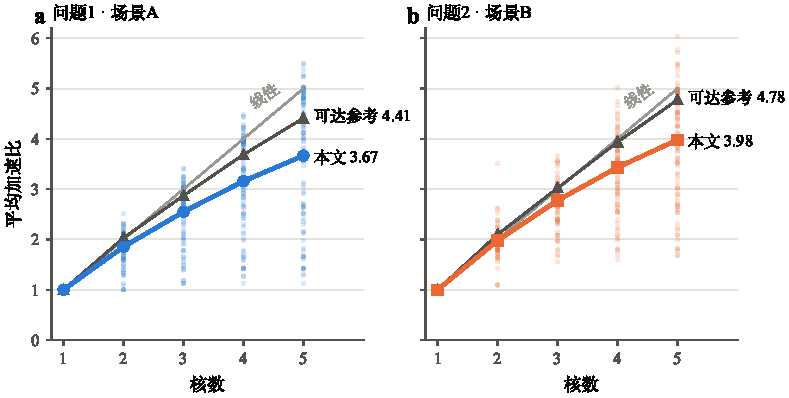
\includegraphics[width=\textwidth]{speedup_p12}
  \caption{1--5 核平均加速比（相对官方单核基准）。淡色点为逐用例加速比，三角为含同步可达参考。(a) 问题一；(b) 问题二}
  \label{fig:speedup}
\end{figure}

\begin{table}[H]
\centering
\caption{问题一结果统计（100 个用例）}
\label{tab:p1-result}
\renewcommand\arraystretch{1.15}
\begin{tabular}{lcccc}
\toprule
 & 2 核 & 3 核 & 4 核 & 5 核 \\
\midrule
平均加速比 & \V{p1_k2_final_mean} & \V{p1_k3_final_mean} & \V{p1_k4_final_mean} & \V{p1_k5_final_mean} \\
最小 / 最大加速比 & \V{p1_k2_final_min} / \V{p1_k2_final_max} & \V{p1_k3_final_min} / \V{p1_k3_final_max} & \V{p1_k4_final_min} / \V{p1_k4_final_max} & \V{p1_k5_final_min} / \V{p1_k5_final_max} \\
平均并行效率 $\bar\rho_k/k$ & \V{p1_k2_eff_mean} & \V{p1_k3_eff_mean} & \V{p1_k4_eff_mean} & \V{p1_k5_eff_mean} \\
对可达参考的达成率 & \V{p1_k2_achieve_mean} & \V{p1_k3_achieve_mean} & \V{p1_k4_achieve_mean} & \V{p1_k5_achieve_mean} \\
平均额外搬运量 / MB & \V{p1_k2_added_MB_mean} & \V{p1_k3_added_MB_mean} & \V{p1_k4_added_MB_mean} & \V{p1_k5_added_MB_mean} \\
子图数中位数 & \V{p1_k2_nsg_median} & \V{p1_k3_nsg_median} & \V{p1_k4_nsg_median} & \V{p1_k5_nsg_median} \\
超线性用例数（$\rho_k>k$） & \V{p1_k2_superlinear} & \V{p1_k3_superlinear} & \V{p1_k4_superlinear} & \V{p1_k5_superlinear} \\
\bottomrule
\end{tabular}
\end{table}

分类来看（图~\ref{fig:heatmap}），III 类 5 核平均 \V{p1_k5_famIII_mean}、达成率 \V{p1_k5_famIII_achieve}，已接近可达水平；II 类为 \V{p1_k5_famII_mean}；I 类只有 \V{p1_k5_famI_mean}，达成率 \V{p1_k5_famI_achieve}。短板集中在 I 类中规模较小的用例。case\_064 的单核基准只有 19{,}116 周期，2--5 核的最优加速比都是 1.13，多给的核心已经用不上：一次跨核等待 1000 周期，与整个计算时间同一量级，场景 A 下几乎无法从切分中获益。图~\ref{fig:bounds} 把每个用例的实测加速比与可达参考放在一起，III 类的点贴近对角线，I 类的点大多在对角线下方。

\begin{figure}[H]
  \centering
  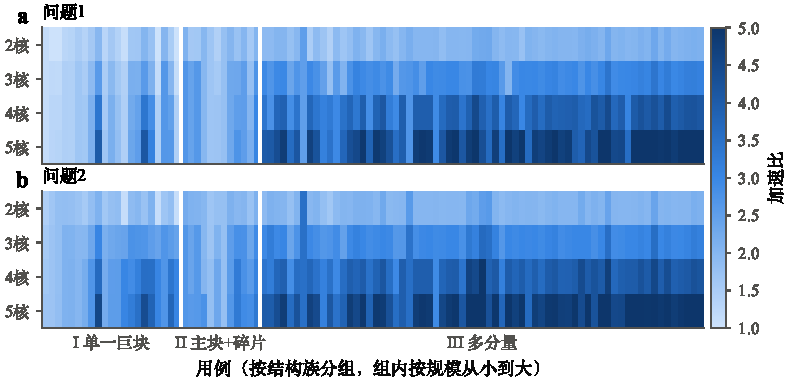
\includegraphics[width=\textwidth]{speedup_heatmap}
  \caption{逐用例加速比热力图（相对官方单核基准）。按类别分组，组内按规模从小到大排列}
  \label{fig:heatmap}
\end{figure}

\begin{figure}[H]
  \centering
  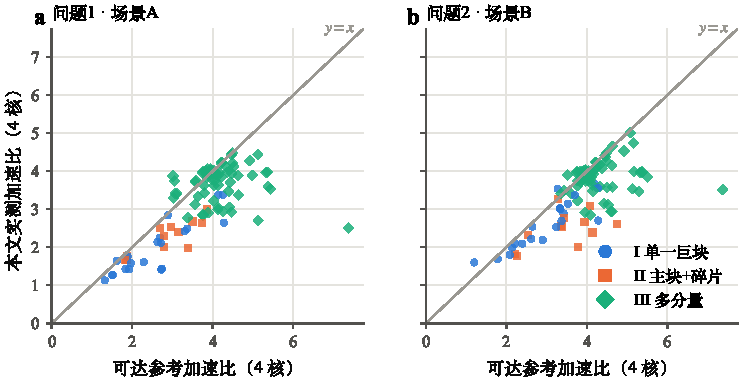
\includegraphics[width=\textwidth]{bounds_gap}
  \caption{逐用例实测加速比与含同步可达参考（4 核）。可达参考为贪心结果，少数点位于对角线上方}
  \label{fig:bounds}
\end{figure}

最终方案的来源见图~\ref{fig:wins}。问题一中成组合并是最主要的来源（\V{source_mix_by_problem_1_coarsen} 组），其次是局部搜索（\V{source_mix_by_problem_1_localsearch} 组）和相位构造（\V{source_mix_by_problem_1_phase} 组）。构造算法给出了好的起点，合并同核相邻子图、缩短依赖链上 Task 序列的后处理贡献了后一段提升。

\begin{figure}[H]
  \centering
  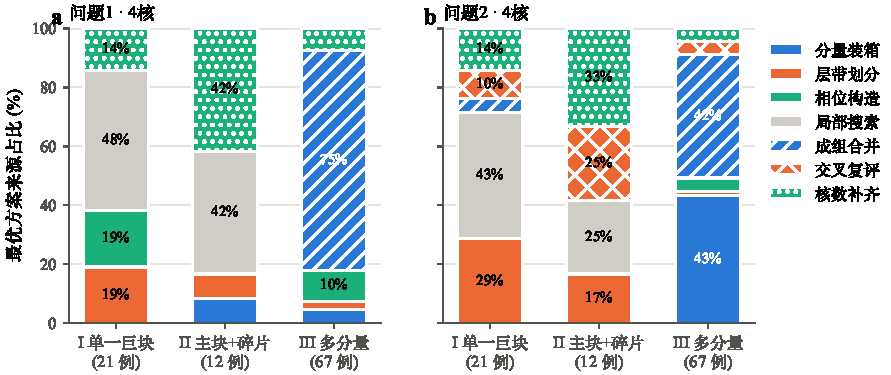
\includegraphics[width=\textwidth]{algo_wins}
  \caption{各类别中最终方案的来源（4 核）。后处理来源单独统计，不归入底层构造算法}
  \label{fig:wins}
\end{figure}

以 I 类中的 case\_002 为例看问题一的求解过程。它有 \V{cs_ops} 个可分配操作，宽度比 \V{cs_width}，单核基准 Makespan 为 \V{cs_single}。表~\ref{tab:case002-p1} 列出它在 4 核下各构造算法的最优结果。朴素分量装箱的加速比恰好为 1：整张图只有一个分量，$\alpha=0.25$ 时不被切开，全部落在一个核上。层带划分最好的 $W=\V{cs_p1_band_div}$ 也只有 \V{cs_p1_band_sp}，因为每个层带子图都是一个 Task，边界往返和激活等待抵消了并行收益。最好的构造是相位构造，且取很大的惩罚 $\lambda=\V{cs_p1_phase_div}$：这张图依赖很密，只在少数位置跨核最划算。最终方案只有 \V{cs_p1_final_nsg} 个子图，Makespan 为 \V{cs_p1_final_ms}。它的逐核时间线见图~\ref{fig:final-tl-p1}：核 0 完成主体计算后空等了近一万周期，才开始最后一个依赖其他核心结果的子图，这段空闲就是跨核激活等待与边界往返的代价，对应式 \eqref{eq:path-bound} 中的 $h\,\delta_{\mathrm{cross}}$ 项。

\begin{table}[H]
\centering
\caption{case\_002 在问题一下的结果（4 核；括号内为胜出参数）}
\label{tab:case002-p1}
\renewcommand\arraystretch{1.15}
\begin{tabular}{lcc}
\toprule
方法 & Makespan & 加速比 \\
\midrule
朴素分量装箱（$\alpha=0.25$） & \V{cs_p1_naive_ms} & \V{cs_p1_naive_sp} \\
分量装箱最优（$\alpha=\V{cs_p1_lpt_div}$） & \V{cs_p1_lpt_ms} & \V{cs_p1_lpt_sp} \\
层带划分最优（$W=\V{cs_p1_band_div}$） & \V{cs_p1_band_ms} & \V{cs_p1_band_sp} \\
相位构造最优（$\lambda=\V{cs_p1_phase_div}$） & \V{cs_p1_phase_ms} & \V{cs_p1_phase_sp} \\
最终方案 & \V{cs_p1_final_ms} & \V{cs_p1_final_sp} \\
\bottomrule
\end{tabular}
\end{table}

\begin{figure}[H]
  \centering
  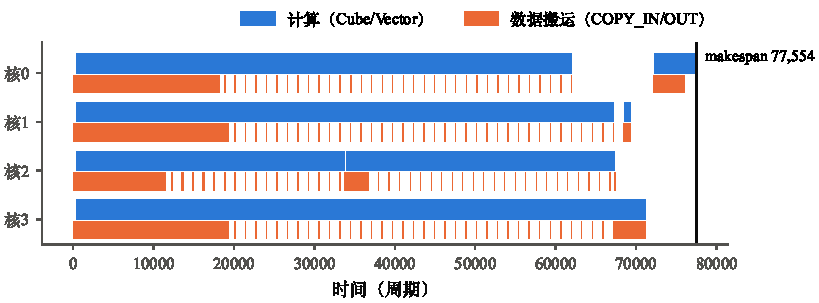
\includegraphics[width=\textwidth]{final_timeline_p1}
  \caption{case\_002 问题一最终方案（4 核）的逐核时间线。每核上条为计算流水线，下条为搬运流水线}
  \label{fig:final-tl-p1}
\end{figure}

\label{sec:neg}除上述三种构造外，实验中还否定过两条构造路线：一是把单入单出链收缩后，仍按操作粒度做通信感知表调度；二是沿最重边做链聚类，簇图成环后再做强连通缩点。为了可比，我们在每类各取 4 个、共 12 个用例上，于 4 核下与逐用例选优比较 Makespan（比值大于 1 表示更慢，取几何平均），结果见表~\ref{tab:negative}。两条路线的共同问题是子图太多，而且切断的恰恰是依赖链，商图路径因此变长，与命题~\ref{prop:path} 的判断一致。

\begin{table}[H]
\centering
\caption{未采用的构造路线（12 个用例，4 核；比值为该方法与逐用例选优的 Makespan 之比）}
\label{tab:negative}
\renewcommand\arraystretch{1.15}
\begin{tabularx}{\textwidth}{l c c c X}
\toprule
路线 & 问题 & 比值几何均值 & 最大子图数 & 失败原因 \\
\midrule
链收缩 + 表调度 & 一 & \V{neg_sched_p1_geo} & \V{neg_sched_p1_nsg_max} & 仍按操作粒度分核，子图碎成上千个，激活等待沿路径累积 \\
 & 二 & \V{neg_sched_p2_geo} & \V{neg_sched_p2_nsg_max} & 同上，跨核同步延迟累积 \\
最重边链聚类 + 缩点 & 一 & \V{neg_cluster_p1_geo} & \V{neg_cluster_p1_nsg_max} & 缩点后合法但子图仍多；仅 \V{neg_cluster_p1_nbetter} 例优于选优 \\
 & 二 & \V{neg_cluster_p2_geo} & \V{neg_cluster_p2_nsg_max} & 同上 \\
\bottomrule
\end{tabularx}
\end{table}

\label{sec:p1-check}下面检验模型本身。命题~\ref{prop:path} 断言场景 A 的代价取决于依赖路径上的子图边界，而不是子图总数。我们用两组数据检验。第一组是扫描阶段 4 核的全部 \V{figx_nsg_pairs} 个候选方案：以每个用例的最优候选为基准计算 Makespan 比值，按子图数分组取中位数（图~\ref{fig:nsg}）。问题一的曲线没有随子图数单调上升，1024 个以上子图的方案（中位 \V{figx_nsg_p1_median_5}）反而好于 16--63 个子图的方案（中位 \V{figx_nsg_p1_median_2}）；256 个以上子图的候选中约 \V{figx_nsg_hi_famIII_pct} 来自 III 类，它们切开的主要是互不相连的分量，没有拉长依赖路径。

\begin{figure}[H]
  \centering
  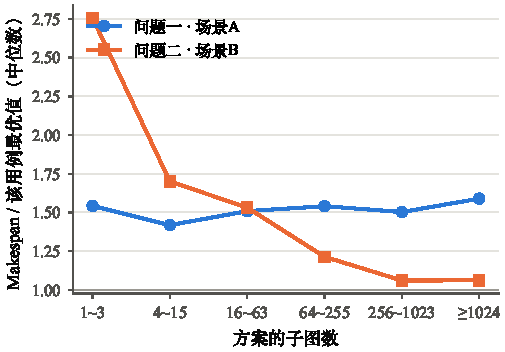
\includegraphics[width=0.66\textwidth]{nsg_quality}
  \caption{子图数与方案质量（4 核，扫描阶段全部候选）。纵轴为候选 Makespan 与该用例最优候选之比的中位数}
  \label{fig:nsg}
\end{figure}

第二组直接度量路径深度。对最终方案，在商图上按拓扑序动态规划求出最长路径上的换核次数
\begin{equation}
  h=\max_{\text{商图路径 } s_1\to\cdots\to s_m}\ \sum_{i=1}^{m-1}\chi_{s_is_{i+1}},
  \label{eq:cross-depth}
\end{equation}
其中 $\chi_{s_is_{i+1}}$ 与式 \eqref{eq:phase} 中的定义相同，相邻子图不同核时为 1。按拓扑序对每个子图记录“到达它的路径上最多换过几次核”，每条边只需做一次比较，所以一次遍历即可求出 $h$。把它与实测 Makespan 超出零通信表调度的部分对比（图~\ref{fig:depth}）。问题一中 \V{figx_depth_p1_zero} 个方案 $h=0$，即所有跨子图依赖都留在同一核心；其余方案的超出量与 $h\,\delta_{\mathrm{cross}}$ 在对数尺度上的相关系数为 \V{figx_depth_p1_corr}，全部 \V{figx_depth_p1_n} 个点都位于对角线上方，即超出量至少为 $h\,\delta_{\mathrm{cross}}$，与式 \eqref{eq:path-bound} 一致。

\begin{figure}[H]
  \centering
  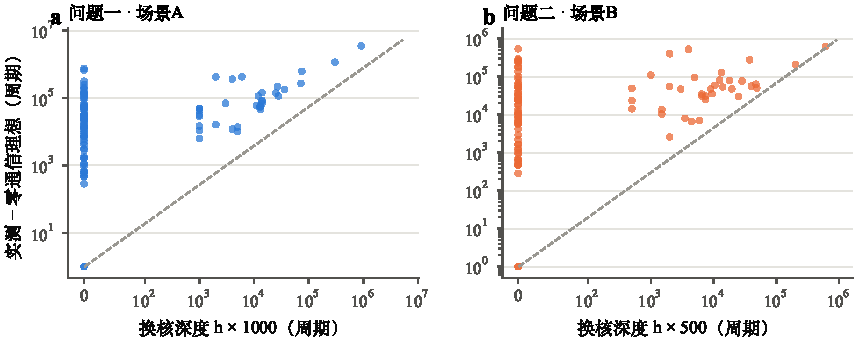
\includegraphics[width=\textwidth]{cross_depth}
  \caption{最终方案的换核深度与 Makespan 超出量（4 核）。横轴为 $h$ 乘以跨核固定延迟，纵轴为实测 Makespan 减去零通信表调度 Makespan；虚线为 $y=x$。(a) 问题一；(b) 问题二}
  \label{fig:depth}
\end{figure}

\subsection{问题二求解思路}

场景 B 有核间同步机制，同一核心上的全部子图合并成一个 Task（图~\ref{fig:sceneAB}(b)）。与场景 A 相比有三处变化。同核子图之间的数据留在 L1/UB 中直接复用，不再经 DDR 往返，同核边界不产生任何搬运。跨核依赖由源核插入 COPY\_OUT、目标核插入 COPY\_IN，目标 COPY\_IN 要在源 COPY\_OUT 完成后再等 $\delta_B=500$ 周期才进入就绪判定，按子图计的激活等待不再存在。全核只有一个 Task，核内调度器面对的是该核全部子图拼成的大图，跨越多个子图的驻留数据会一直占着缓存，容量不够时就插入换入换出。

前两处变化让细分切图变得便宜，第三处又给细分和合并都设了限。求解思路是：保留问题一的决策变量与合法性约束，把边界搬运从子图边界改为核边界，把时间约束从子图激活改为操作级的跨核同步，并加入缓存驻留约束；由修正后的模型判断参数应向哪个方向移动，再沿用问题一的三种构造算法与选优框架。后处理中成组合并的作用在场景 B 下有所不同，需要重新分析。由于问题二、三同属场景 B，两问的候选方案还可以互相复评。

\subsection{问题二模型建立}\label{sec:p2-model}

\subsubsection{边界搬运量的修正}

场景 B 下只有跨核的张量需要搬运。把式 \eqref{eq:copies-A} 中的子图映射 $\sg$ 换成核心映射 $\core$，得到
\begin{equation}
  n^{\mathrm{in}}_t=\big|\core(U_t)\setminus \core(P_t)\big|,\qquad
  n^{\mathrm{out}}_t=\big|\{\,n\in \core(P_t):\ t\in T_{\mathrm{out}}\ \text{或}\ \core(U_t)\setminus\{n\}\ne\varnothing\,\}\big| ,
  \label{eq:copies-B}
\end{equation}
\begin{equation}
  Q_B=\sum_{t\in T} s_t\big(n^{\mathrm{in}}_t+n^{\mathrm{out}}_t\big)-Q_{\mathrm{orig}} .
  \label{eq:QB}
\end{equation}
推理与式 \eqref{eq:copies-A} 相同，只是边界的单位变了：场景 B 中同一核心上的子图属于同一个 Task，张量在核内生产、在核内使用时不需要搬运；只有当某个核心要用到别的核心生产的张量时，才需要一次读入，而生产它的核心只要有别的核心使用它（或它是图输出）就要写出一次。所以把式 \eqref{eq:copies-A} 中的子图集合 $\sg(\cdot)$ 换成核心集合 $\core(\cdot)$，就得到场景 B 的搬运次数，再逐张量求和并减去原图已有的 COPY 字节，即得式 \eqref{eq:QB}。

\begin{proposition}\label{prop:qb}
对同一份方案，场景 B 的边界搬运量不超过场景 A，即 $Q_B\le Q_A$。
\end{proposition}
\begin{proof}
核心映射是子图映射的复合，$\core(v)=\core(\sg(v))$，所以对任意操作集合 $X$ 有 $|\core(X)|\le|\sg(X)|$。对读入次数，若核心 $n\in\core(U_t)\setminus\core(P_t)$，则 $n$ 上消费 $t$ 的子图都不在 $\sg(P_t)$ 中，即 $\core(U_t)\setminus\core(P_t)\subseteq \core\big(\sg(U_t)\setminus\sg(P_t)\big)$，于是场景 B 的 $n^{\mathrm{in}}_t$ 不超过场景 A。对写出次数，场景 B 中每个计入的生产核心至少对应一个满足场景 A 计入条件的生产子图，且不同核心对应的子图互不相同，故也不超过场景 A。逐张量相加即得。
\end{proof}

命题~\ref{prop:qb} 意味着切得越细，两种场景的差距越大：子图数增加时 $Q_A$ 随子图边界增长，$Q_B$ 只随核边界增长。图~\ref{fig:trafficAB} 用同一方案在两种场景下的 \V{fig_traffic_pairs} 组配对评估验证了这一点：子图数在 512 个以上时，场景 B 的额外搬运量只有场景 A 的 \V{fig_traffic_added_ratio_4}，Makespan 为场景 A 的 \V{fig_traffic_ms_ratio_4}。

\begin{figure}[H]
  \centering
  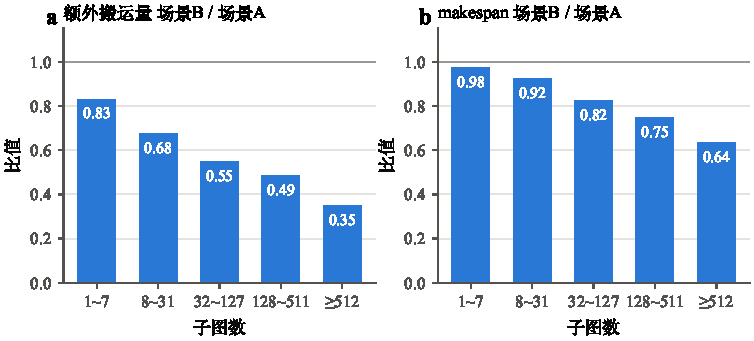
\includegraphics[width=\textwidth]{traffic_AB}
  \caption{同一方案在场景 A、B 下的配对对比（按子图数分组）}
  \label{fig:trafficAB}
\end{figure}

\subsubsection{时间模型的修正}

场景 B 中子图不再单独激活，时间约束落在操作上。对跨核依赖 $(u,v)$，设 $u$ 的输出张量为 $t$，则
\begin{equation}
  S_v\ \ge\ f_u+\frac{s_t}{B_u^{\mathrm{eff}}}+\delta_B+\frac{s_t}{B_v^{\mathrm{eff}}},
  \label{eq:sync-B}
\end{equation}
同核依赖只需 $S_v\ge f_u$。$B^{\mathrm{eff}}$ 为 COPY 执行时实际分到的带宽。式 \eqref{eq:sync-B} 按跨核数据的实际流程逐段相加：$u$ 完成后，源核的 COPY\_OUT 把 $t$ 写回 DDR，耗时 $s_t/B_u^{\mathrm{eff}}$；写完后要等同步延迟 $\delta_B$，目标核的 COPY\_IN 才进入就绪判定；再读入 $t$，耗时 $s_t/B_v^{\mathrm{eff}}$，之后 $v$ 才能开始。按题目附录 D.5，所有访问 DDR 的搬运公平共享总带宽。设时刻 $\tau$ 有 $m(\tau)$ 个 DDR 搬运在途，第 $j$ 个的剩余字节数为 $w_j(\tau)$，则每个在途搬运分到 $B/m(\tau)$ 的带宽：
\begin{equation}
  \frac{\mathrm{d}w_j}{\mathrm{d}\tau}=-\frac{B}{m(\tau)},\qquad
  e_j=\min\{\tau:\ w_j(\tau)=0\}.
  \label{eq:fair-share}
\end{equation}
从发射时刻 $a_j$ 到完成时刻 $e_j$ 对上式积分，得 $s_j=\int_{a_j}^{e_j}B/m(\tau)\,\mathrm{d}\tau$，于是这次搬运的平均带宽为
\begin{equation}
  B^{\mathrm{eff}}_j=\frac{s_j}{e_j-a_j}=\frac{1}{e_j-a_j}\int_{a_j}^{e_j}\frac{B}{m(\tau)}\,\mathrm{d}\tau\ \le\ B ,
  \label{eq:beff}
\end{equation}
不等号是因为 $m(\tau)\ge 1$。$m(\tau)$ 只在有搬运加入或完成时改变，评估程序按事件逐段结算。跨核搬运的实际耗时因此不只取决于自身字节数，还取决于同一时段有多少搬运在争用带宽，这也是式 \eqref{eq:sync-B} 中 $B^{\mathrm{eff}}$ 写不成常数的原因。沿任意一条依赖路径 $v_1\to v_2\to\cdots\to v_m$，同核的相邻操作满足 $S_{v_{i+1}}\ge f_{v_i}$，跨核的相邻操作满足式 \eqref{eq:sync-B}；由式 \eqref{eq:beff}，$B^{\mathrm{eff}}\le B$，所以每次跨核至少多出 $\delta_B+2s_t/B$。再由 $f_{v_i}\ge S_{v_i}+c_{v_i}$ 沿路径累加，若路径换核 $h$ 次，则
\begin{equation}
  M_k\ \ge\ \sum_{i=1}^{m} c_{v_i}+h\Big(\delta_B+\frac{2\,\bar s}{B}\Big),
  \label{eq:path-B}
\end{equation}
$\bar s$ 为路径上跨核张量的最小字节数。与式 \eqref{eq:path-bound} 相比，这里的代价只与换核次数有关，与子图数无关。场景 B 中真正要控制的是换核深度，同核上切出多少子图本身不付代价。

\subsubsection{缓存驻留约束}

场景 B 的另一部分代价在核内。设核心 $n$ 上合并后 Task 的操作按核内调度顺序排为 $o_1,o_2,\dots$，张量 $t$ 从生产者完成到该核上最后一个消费者开始都驻留在缓存中，驻留区间与第 $j$ 步的驻留量为
\begin{equation}
  \mathcal{L}_t=\big[f_{P_t},\ \max_{v\in U_t,\ \core(v)=n} S_v\big],\qquad
  \Phi_n(j)=\sum_{t:\ o_j\in\mathcal{L}_t} s_t .
  \label{eq:live}
\end{equation}
张量从生产出来到最后一次被该核使用之前都不能丢弃，所以它在 $\mathcal{L}_t$ 内一直占用缓存，第 $j$ 步的占用量就是所有驻留区间覆盖 $o_j$ 的张量字节之和。按张量所在的缓存分别求和，必须满足
\begin{equation}
  \Phi_n^{L1}(j)\le C_{L1},\qquad \Phi_n^{UB}(j)\le C_{UB},\qquad \forall n,\ j .
  \label{eq:resident}
\end{equation}
不满足时，调度器按“下一次使用最晚者先换出”的规则（即 Belady 规则\cite{belady1966study}）插入换出与换入，产生额外搬运 $Q^{\mathrm{sp}}$。在场景 A 中，一个张量最多驻留到所在子图结束；在场景 B 中，生产者在第 $i$ 个子图、消费者在第 $j$ 个子图的张量，要跨过中间 $j-i-1$ 个子图一直占着缓存。所以场景 B 的同核排序不仅影响依赖等待，还直接决定驻留压力。图~\ref{fig:spill} 把 \V{fig_spill_pairs} 组同方案配对按中间张量总量分组：中间张量越多，场景 B 触发换出的比例越高（从 \V{fig_spill_trigger_pct_0} 升到 \V{fig_spill_trigger_pct_2} 以上），场景 B 相对场景 A 的 Makespan 优势也从 \V{fig_spill_ms_ratio_0} 收窄到 \V{fig_spill_ms_ratio_3}。

\begin{figure}[H]
  \centering
  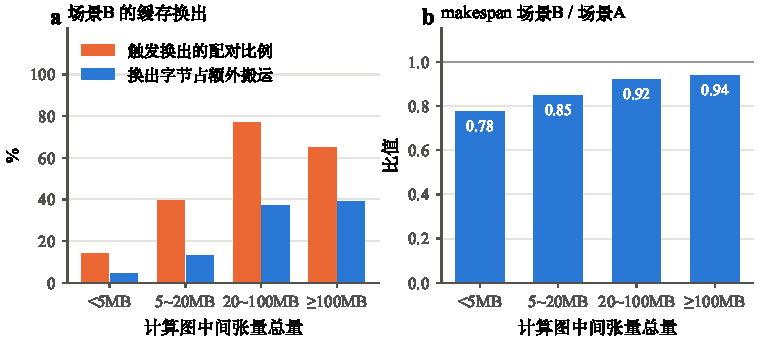
\includegraphics[width=\textwidth]{spill_B}
  \caption{场景 B 的缓存换出。(a) 按中间张量总量分组，触发换出的配对比例与换出字节占额外搬运的比例；(b) 场景 B 相对场景 A 的 Makespan 之比}
  \label{fig:spill}
\end{figure}

综合以上修正，问题二的模型为
\begin{equation}
\begin{aligned}
  \min\quad & M_k=\max_{v\in\Oe} f_v\\
  \text{s.t.}\quad & \text{划分、无环与同核顺序约束 \eqref{eq:assign}--\eqref{eq:order}},\\
  & S_v\ge f_u\ \ (\core(u)=\core(v)),\quad \text{跨核同步约束 \eqref{eq:sync-B}，带宽共享 \eqref{eq:fair-share}},\\
  & f_v\ge S_v+c_v,\quad \text{缓存驻留约束 \eqref{eq:resident}},
\end{aligned}
  \label{eq:obj-p2}
\end{equation}
次要目标为 $Q_B+Q^{\mathrm{sp}}$。它与问题一共用合法性约束，命题~\ref{prop:acyclic} 的结论不变，三种构造算法可以直接使用；变化的是参数的合适区域和后处理的作用。

\subsection{问题二模型求解与结果分析}

\subsubsection{算法描述}

构造阶段沿用算法~\ref{alg:lpt}--\ref{alg:select} 与相同的参数网格，式 \eqref{eq:path-B} 预测最优方案会切得更细：层带数 $W$ 应偏大，相位构造的惩罚 $\lambda$ 此时对应 500 周期同步加上张量传输时间，应比问题一小。\label{sec:p2-coarsen}后处理中，成组合并在场景 B 下的作用需要重新分析。场景 B 下每核本来就只有一个 Task，成组合并既不改变 Task 数，也不改变跨核边界，它改变的是核内执行顺序。评估程序先对整个核的计算图做确定性拓扑排序（题目附录 C 的步骤 1），再按 \texttt{core\_schedules} 中的子图次序做稳定排序：不同子图按给定次序先后排开，同一子图内部保留拓扑排序的相对顺序。把相邻 $w$ 个子图合并后，它们的操作落进同一个桶，按全局拓扑序交错排列，原本前后串行的几条独立链可以穿插执行，张量的驻留区间随之改变，换出量和流水线空闲都可能下降。

除成组合并外，问题二还增加了交叉复评。问题二、三同属场景 B，方案可以互换。我们把问题三各来源的获胜方案交给问题二的评估程序，反之亦然，按方案内容的哈希去重，避免重复评估。它相当于在算法~\ref{alg:select} 的核数补齐之前把候选集扩大为 $\{x\}\cup\{x^{(3)}_{k}\}$，$x^{(3)}_{k}$ 为问题三的已选方案。核数补齐的做法与问题一相同。

\subsubsection{求解分析}

扫描数据支持“场景 B 应切得更细”的判断。图~\ref{fig:nsg} 中问题二的曲线随子图数单调下降：1--3 个子图的候选 Makespan 中位数是该用例最优值的 \V{figx_nsg_p2_median_0} 倍，256 个以上子图的候选只有 \V{figx_nsg_p2_median_4} 倍，5 核最终方案的子图数中位数为 \V{p2_k5_nsg_median}，相位构造胜出的 $\lambda$ 中位数为 \V{p2_phase_bestlam_median}。换核深度仍然起作用，这与式 \eqref{eq:path-B} 一致：图~\ref{fig:depth}(b) 中最终方案的超出量与 $h\,\delta_B$ 的对数相关系数为 \V{figx_depth_p2_corr}，\V{figx_depth_p2_n} 个点中有 \V{figx_depth_p2_above} 个位于对角线上方。也就是说，问题二要控制的是换核深度，而不是子图个数。

表~\ref{tab:algo-p2} 与图~\ref{fig:algocmp}(b) 给出各构造算法与逐用例选优的对比。任何单一算法都落后于选优：5 核时最好的单一算法（分量装箱）为 \V{p2_k5_lpt_mean}，逐用例选优为 \V{p2_k5_portfolio_mean}。层带划分在 I 类上 4 核平均达到 \V{p2_k4_famI_band_mean}，同核层带之间的数据不再往返 DDR，是它在场景 B 中表现好的原因。后处理方面，成组合并在 \V{co1_p2_groups} 组里改进了 \V{co1_p2_improved} 组，平均缩短 \V{co1_p2_mean_red_pct}，最多 \V{co1_p2_max_red_pct}；局部搜索起点可追溯的 \V{ls_p2_jobs} 个作业平均缩短 \V{ls_p2_mean_red_pct}；最终方案中有 \V{source_mix_by_problem_2_crosseval} 组来自交叉复评；核数补齐评估了 \V{mono_p2} 个补空核方案，补齐后每个用例的加速比都随核数单调不减。

\begin{table}[H]
\centering
\caption{问题二：单一构造算法与逐用例选优的平均加速比}
\label{tab:algo-p2}
\renewcommand\arraystretch{1.15}
\begin{tabular}{lcccc}
\toprule
方法 & 2 核 & 3 核 & 4 核 & 5 核 \\
\midrule
朴素基线（分量装箱，$\alpha=0.25$） & \V{p2_k2_naive_mean} & \V{p2_k3_naive_mean} & \V{p2_k4_naive_mean} & \V{p2_k5_naive_mean} \\
分量装箱 & \V{p2_k2_lpt_mean} & \V{p2_k3_lpt_mean} & \V{p2_k4_lpt_mean} & \V{p2_k5_lpt_mean} \\
层带划分 & \V{p2_k2_band_mean} & \V{p2_k3_band_mean} & \V{p2_k4_band_mean} & \V{p2_k5_band_mean} \\
相位构造 & \V{p2_k2_phase_mean} & \V{p2_k3_phase_mean} & \V{p2_k4_phase_mean} & \V{p2_k5_phase_mean} \\
逐用例选优 & \V{p2_k2_portfolio_mean} & \V{p2_k3_portfolio_mean} & \V{p2_k4_portfolio_mean} & \V{p2_k5_portfolio_mean} \\
加后处理（最终） & \V{p2_k2_final_mean} & \V{p2_k3_final_mean} & \V{p2_k4_final_mean} & \V{p2_k5_final_mean} \\
\bottomrule
\end{tabular}
\end{table}

问题二 2--5 核平均加速比依次为 \V{p2_k2_final_mean}、\V{p2_k3_final_mean}、\V{p2_k4_final_mean}、\V{p2_k5_final_mean}（图~\ref{fig:speedup}(b)），5 核相对朴素基线提高 \V{p2_k5_naive_gain_pct}，对可达参考的平均达成率 \V{p2_k5_achieve_mean}。更完整的统计见表~\ref{tab:p2-result}，逐用例结果见附录 B。快速模式下只用 9 个构造候选，2--5 核平均加速比为 \V{figx_fast_p2_k2_mean}、\V{figx_fast_p2_k3_mean}、\V{figx_fast_p2_k4_mean}、\V{figx_fast_p2_k5_mean}，5 核已接近最终结果，在最大用例上一次运行的 CPU 时间约 \V{figx_fast_big_cpu_min} 分钟，满足题目对高效的要求。

\begin{table}[H]
\centering
\caption{问题二结果统计（100 个用例）}
\label{tab:p2-result}
\renewcommand\arraystretch{1.15}
\begin{tabular}{lcccc}
\toprule
 & 2 核 & 3 核 & 4 核 & 5 核 \\
\midrule
平均加速比 & \V{p2_k2_final_mean} & \V{p2_k3_final_mean} & \V{p2_k4_final_mean} & \V{p2_k5_final_mean} \\
最小 / 最大加速比 & \V{p2_k2_final_min} / \V{p2_k2_final_max} & \V{p2_k3_final_min} / \V{p2_k3_final_max} & \V{p2_k4_final_min} / \V{p2_k4_final_max} & \V{p2_k5_final_min} / \V{p2_k5_final_max} \\
平均并行效率 & \V{p2_k2_eff_mean} & \V{p2_k3_eff_mean} & \V{p2_k4_eff_mean} & \V{p2_k5_eff_mean} \\
对可达参考的达成率 & \V{p2_k2_achieve_mean} & \V{p2_k3_achieve_mean} & \V{p2_k4_achieve_mean} & \V{p2_k5_achieve_mean} \\
平均额外搬运量 / MB & \V{p2_k2_added_MB_mean} & \V{p2_k3_added_MB_mean} & \V{p2_k4_added_MB_mean} & \V{p2_k5_added_MB_mean} \\
子图数中位数 & \V{p2_k2_nsg_median} & \V{p2_k3_nsg_median} & \V{p2_k4_nsg_median} & \V{p2_k5_nsg_median} \\
\bottomrule
\end{tabular}
\end{table}

分类别的结果见表~\ref{tab:family}。I 类依赖密集，朴素基线在这一类上几乎等于单核，因为分量装箱以连通分量为单位分核，整张图只有一个分量时所有工作都落在同一个核上；场景 B 下同核子图之间不付代价，只要控制住跨核边，层带划分和相位构造都能在分量内部找到并行性，I 类的提升因此最大。III 类本来就可以按分量并行，朴素基线已经不差，提升空间较小。

\begin{table}[H]
\centering
\caption{问题二各类别的规模与 4 核平均加速比}
\label{tab:family}
\renewcommand\arraystretch{1.15}
\begin{tabular}{lccccc}
\toprule
类别 & 用例数 & 操作数中位 & 宽度比中位 & 朴素基线 & 本文 \\
\midrule
I 单一巨块 & \V{family_count_I} & \V{famI_ops_median} & \V{famI_width_median} & \V{p2_k4_famI_naive_mean} & \V{p2_k4_famI_mean} \\
II 主块+碎片 & \V{family_count_II} & \V{famII_ops_median} & \V{famII_width_median} & \V{p2_k4_famII_naive_mean} & \V{p2_k4_famII_mean} \\
III 多分量 & \V{family_count_III} & \V{famIII_ops_median} & \V{famIII_width_median} & \V{p2_k4_famIII_naive_mean} & \V{p2_k4_famIII_mean} \\
\bottomrule
\end{tabular}
\end{table}

仍以 case\_002 为例。表~\ref{tab:case002} 列出它在问题二下 4 核各构造算法的最优结果。朴素分量装箱的加速比为 1，原因与问题一相同；层带划分只用 $W=\V{cs_p2_band_div}$ 个层带就达到 \V{cs_p2_band_sp}，同核层带之间的数据留在核内，切带不再付出边界往返的代价。这个用例的最优 $W$ 很小，与平均趋势相反，说明参数只能逐用例选。最好的构造仍是相位构造，惩罚取 $\lambda=\V{cs_p2_phase_div}$；最终方案有 \V{cs_p2_final_nsg} 个子图，额外搬运量不到 1~MB。它的逐核时间线见图~\ref{fig:final-tl-p2}：四个核心几乎同时结束，尾部的等待很短，搬运流水线上只剩跨核依赖和图输入输出的搬运，Makespan 为 \V{figx_tl_case_002_p2_ms}。

\begin{table}[H]
\centering
\caption{case\_002 在问题二下的结果（4 核；括号内为胜出参数）}
\label{tab:case002}
\renewcommand\arraystretch{1.15}
\begin{tabular}{lcc}
\toprule
方法 & Makespan & 加速比 \\
\midrule
朴素分量装箱（$\alpha=0.25$） & \V{cs_p2_naive_ms} & \V{cs_p2_naive_sp} \\
分量装箱最优（$\alpha=\V{cs_p2_lpt_div}$） & \V{cs_p2_lpt_ms} & \V{cs_p2_lpt_sp} \\
层带划分最优（$W=\V{cs_p2_band_div}$） & \V{cs_p2_band_ms} & \V{cs_p2_band_sp} \\
相位构造最优（$\lambda=\V{cs_p2_phase_div}$） & \V{cs_p2_phase_ms} & \V{cs_p2_phase_sp} \\
最终方案 & \V{cs_p2_final_ms} & \V{cs_p2_final_sp} \\
\bottomrule
\end{tabular}
\end{table}

\begin{figure}[H]
  \centering
  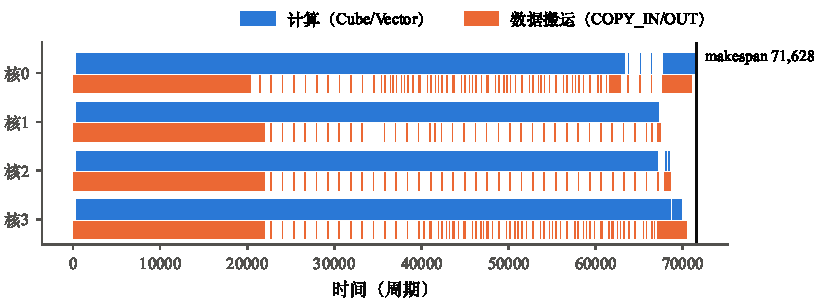
\includegraphics[width=\textwidth]{final_timeline_p2}
  \caption{case\_002 问题二最终方案（4 核）的逐核时间线。每核上条为计算流水线，下条为搬运流水线}
  \label{fig:final-tl-p2}
\end{figure}

\subsection{问题三求解思路}

问题三在场景 B 的基础上增加一块所有核心共享的只读 L2 Cache，容量 $C_{L2}=1{,}048{,}576$ 字节，带宽 $B_{L2}=250$ bytes/cycle，与 DDR 带宽相互独立。根据题目附录 D.5 与评估程序的实现，它的规则可以归纳为四条：只有 COPY\_IN 查询缓存，COPY\_OUT 总是写 DDR，查询发生在 COPY\_IN 发射时刻，键为逻辑张量编号，同一张量被不同核心读取时键相同；命中的 COPY\_IN 进入缓存带宽池，多个命中公平共享 250 bytes/cycle，不占 DDR 带宽，未命中的走 DDR；未命中的 COPY\_IN 完成后才把张量写入缓存，容量不足时按先进先出淘汰，命中不改变淘汰顺序，大于容量的张量不缓存；命中率按字节计。

这几条规则决定了求解思路。命中需要同一张量此前已被读过、那次读取已经完成、并且之后写入的数据还没把它挤出去，这是时序条件和容量条件；命中省下的是 DDR 带宽，只有 DDR 确实繁忙时才能换来时间。所以我们先写出缓存状态的演化和命中的充要条件，据此把未命中分类，再用 DDR 忙碌占比刻画命中能换来多少时间，并给出缓存加速比的带宽上限。求解上，问题三与问题二同属场景 B，方案可以互换，问题二的全部候选都交给问题三的评估程序复评，再在缓存评估下做后处理。题目要求研究的容量和带宽影响，通过固定一批方案、只改缓存参数重新评估来回答。

\subsection{问题三模型建立}\label{sec:p3-math}

\subsubsection{缓存状态与命中条件}

把缓存内容记为按写入先后排列的队列 $\mathcal{Q}(\tau)=(t_1,t_2,\dots)$，占用 $|\mathcal{Q}|=\sum_{t\in\mathcal{Q}}s_t$。一次未命中的 COPY\_IN 在完成时刻写入张量 $t$（若 $s_t\le C_{L2}$ 且 $t\notin\mathcal{Q}$），写入前先从队首淘汰，直到放得下：
\begin{equation}
  \text{while }\ |\mathcal{Q}|+s_t>C_{L2}:\ \ \mathcal{Q}\leftarrow\mathcal{Q}\setminus\{\text{队首}\};\qquad \mathcal{Q}\leftarrow\mathcal{Q}\oplus t .
  \label{eq:fifo}
\end{equation}
命中的读取与 DDR 读取分别在两个独立的带宽池中按式 \eqref{eq:fair-share} 的方式公平共享：
\begin{equation}
  \frac{\mathrm{d}w_j}{\mathrm{d}\tau}=
  \begin{cases}
  -B_{L2}/m_{L2}(\tau), & j\ \text{命中},\\
  -B/m_{\mathrm{DDR}}(\tau), & j\ \text{未命中或为 COPY\_OUT},
  \end{cases}
  \label{eq:pools}
\end{equation}
即命中的读取只和其他命中读取分享 $B_{L2}$，不占用 DDR；未命中的读取和全部写出仍在 DDR 池中分享 $B$。命中越多，DDR 池中的 $m_{\mathrm{DDR}}(\tau)$ 越小，其余搬运分到的带宽就越大，这是缓存能缩短 Makespan 的途径。字节命中率为
\begin{equation}
  \theta=\frac{\sum_{j\ \text{命中}} s_j}{\sum_{j\ \text{为 COPY\_IN}} s_j}.
  \label{eq:hitrate}
\end{equation}

记第 $j$ 次 COPY\_IN 读取的逻辑张量为 $t_j$，发射、完成时刻为 $a_j,e_j$。它命中当且仅当存在更早的一次未命中读取 $i$（$t_i=t_j$），满足
\begin{equation}
  e_i\le a_j\qquad\text{且}\qquad \sum_{\ell\in\mathcal{I}(e_i,a_j)} s_\ell\ \le\ C_{L2}-s_{t_j},
  \label{eq:hit}
\end{equation}
$\mathcal{I}(e_i,a_j)$ 为在 $(e_i,a_j]$ 内写入缓存的其他张量。第一式是时序条件：张量在未命中读取完成时才写入缓存，而查询发生在发射时刻，所以只有 $e_i\le a_j$ 时第 $j$ 次查询才可能看到它。第二式是容量条件：由式 \eqref{eq:fifo}，张量写入后只会因后来写入的数据而被挤出，命中又不改变队列顺序，只要其后写入的总字节数不超过 $C_{L2}-s_{t_j}$，它就仍在队列中。两个条件同时成立时查询必然命中；反过来，命中的张量一定是某次未命中读取写入且尚未淘汰的，两个条件都成立，所以式 \eqref{eq:hit} 是充要条件。据此把每次未命中分为三类\cite{hill1989evaluating}：
\begin{equation}
  \text{缺失类型}(j)=
  \begin{cases}
  \text{首次缺失}, & \text{此前没有任何读取 } i<j,\ t_i=t_j;\\
  \text{并发缺失}, & \text{存在 } i<j,\ t_i=t_j,\ \text{但所有这样的 } i \text{ 都有 } e_i>a_j;\\
  \text{容量缺失}, & \text{曾经写入，但已被先进先出淘汰。}
  \end{cases}
  \label{eq:miss-class}
\end{equation}
首次缺失由计算图决定，任何调度都消除不了；容量缺失与缓存大小和写入次序有关；并发缺失则完全是时序问题：多个核心几乎同时读同一个张量，第一次读取还没完成，其余读取全部落空，同时挤占 DDR。

\subsubsection{缓存收益与带宽上限}\label{sec:p3-benefit}

一次命中节省的 DDR 占用为 $s_j/B$ 周期，但能否转化为 Makespan 的缩短，取决于 DDR 是不是瓶颈。定义无 L2 时的 DDR 忙碌占比与同一方案的缓存加速比
\begin{equation}
  \beta=\frac{Q_{\mathrm{DDR}}}{B\cdot M^{\mathrm{noL2}}},\qquad
  \gamma=\frac{M^{\mathrm{noL2}}}{M^{\mathrm{cache}}},
  \label{eq:ddr-busy}
\end{equation}
$Q_{\mathrm{DDR}}$ 为全部 DDR 搬运字节数。$\beta$ 很小时 DDR 大部分时间空闲，省下的带宽没有别的搬运去用，命中只让个别 COPY\_IN 快一点，未必落在关键路径上；$\beta$ 接近 1 时，命中直接减轻了争用，所有在途搬运都会变快。所以 $\gamma$ 应随 $\beta$ 上升。进一步，记只读 Cache 配置下仍走 DDR 的字节数为 $Q_D$、命中字节数为 $Q_H$，无 L2 时这些字节全部走 DDR。只读 Cache 下 $M^{\mathrm{cache}}\ge Q_D/B$；若无 L2 时 Makespan 完全由 DDR 带宽决定，即 $M^{\mathrm{noL2}}\approx (Q_D+Q_H)/B$，则
\begin{equation}
  \gamma=\frac{M^{\mathrm{noL2}}}{M^{\mathrm{cache}}}\ \le\ \frac{(Q_D+Q_H)/B}{Q_D/B}=\bar\gamma=1+\frac{Q_H}{Q_D}.
  \label{eq:gamma-bound}
\end{equation}
式 \eqref{eq:gamma-bound} 是带宽完全饱和这一理想情形下的上限，前提不总成立，因此只作估计。缓存也可能让同一方案变慢：命中改变了 COPY\_IN 的完成时刻，而核内操作顺序是固定的，完成时刻的变化可能让关键路径上的某个操作等待更久，这是多处理机调度中已知的时序异常\cite{graham1969bounds}。

\subsubsection{问题三的优化模型}

问题三的决策变量与约束与问题二相同，目标由问题三的评估程序给出：
\begin{equation}
\begin{aligned}
  \min\quad & M_k^{\mathrm{cache}}=\max_{v\in\Oe} f_v\\
  \text{s.t.}\quad & \text{问题二的全部约束 \eqref{eq:assign}--\eqref{eq:order}、\eqref{eq:sync-B}--\eqref{eq:resident}},\\
  & \text{COPY\_IN 按命中条件 \eqref{eq:hit} 选择带宽池 \eqref{eq:pools}，缓存内容按式 \eqref{eq:fifo} 更新},
\end{aligned}
  \label{eq:obj-p3}
\end{equation}
并以同核数下两种配置各自最优方案的缓存加速比
\begin{equation}
  \Gamma_k=\frac{M_k^{\mathrm{noL2,*}}}{M_k^{\mathrm{cache,*}}}
  \label{eq:Gamma}
\end{equation}
作为题目要求报告的指标。由式 \eqref{eq:hit}--\eqref{eq:gamma-bound}，好的问题三方案要同时满足三点：DDR 足够紧张，缓存才有意义；共享同一输入的消费者分散在几个核心上，缓存才有重复读取可以服务；这些读取在时间上错开，命中条件才能成立。前两点会增加跨核依赖，第三点要求读取有先后，三者之间存在张力。

\subsection{问题三模型求解与结果分析}

\subsubsection{算法描述}\label{sec:p3-solve}

问题三的候选池包括问题二的全部候选方案，再加上在问题三评估程序下做的后处理，流程仍为算法~\ref{alg:select}，只是把 $E_p$ 换成问题三的评估程序。第一步是交叉复评。这一步的起因是 case\_061 3 核：问题三原来的最优方案来自相位构造，Makespan 为 36{,}250；问题二中经成组合并（宽度 16、全部核心）得到的方案放到问题三评估程序下只有 28{,}368，缩短 21.7\%。只在本问题的最优起点上做后处理会漏解。因此我们把问题一、二、三各来源的获胜方案按内容哈希去重后，逐个交给问题二、三的评估程序，并在最终阶段把两问的最终方案再互相复评一次，使两种配置在“各自最优”口径下的候选池对称。

第二步是在缓存评估下重做成组合并与局部搜索。成组合并改变同核子图的执行顺序（第~\ref{sec:p2-coarsen} 节），也就改变了共享张量被读取的先后，有可能把并发缺失变成命中，所以在问题三评估程序下重新做一遍。局部搜索以问题三的 Makespan 为目标，优先用于缓存收益潜力大的用例。

另有两条针对缓存的路线在实验中被否定。一是在相位构造中加入缓存感知代价：某张量已被一个核心读过时，其他核心再读按缓存带宽计价，以鼓励把共享张量的消费者分散到多个核心。在第~\ref{sec:neg} 节的 12 个用例上，它相对问题三构造阶段选优的 Makespan 比值几何均值为 \V{neg_phasec_p3_d50000_geo}（$\lambda=5\times10^4$），没有一例更好。它鼓励跨核扇出，增加了跨核边和同步，而同时发起的读取按式 \eqref{eq:hit} 根本不会命中，按缓存带宽计价的前提本身不成立。二是错开读取的后处理：为每个共享张量指定一个领读核心，领读的子图排前、跟读的子图排后，只调整各核内子图的先后。它在并发缺失最多的用例上效果有限，因为锁步读取往往发生在同一条依赖链内部，调整子图顺序改变不了核间的相位差（实验记录见第~\ref{sec:neg-record} 节）。

\subsubsection{求解分析}

先检验缓存收益的影响因素。图~\ref{fig:ddr} 用 \V{fig_ddr_pairs} 组同方案配对检验了 $\gamma$ 与 $\beta$ 的关系：$\beta<20\%$ 时 $\gamma$ 平均只有 \V{fig_ddr_mean_0}，$\beta\ge 80\%$ 时达到 \V{fig_ddr_mean_4}。图~\ref{fig:cbound} 把最终方案（4 核）的实测 $\gamma$ 与上限 $\bar\gamma$ 放在一起：\V{figx_cb_n} 个用例中 \V{figx_cb_below} 个位于上限之下；按实际收益占上限收益的比例 $(\gamma-1)/(\bar\gamma-1)$ 计，$\beta\ge 60\%$ 的用例中位数为 \V{figx_cb_ratio_hi}，$\beta<30\%$ 的用例中位数为 \V{figx_cb_ratio_lo}。命中字节即使不少，DDR 不紧张时也几乎换不来时间。缓存让同一方案变慢的情况在全部 500 组同方案配对中出现了 \V{p3_same_worse_total} 次，最小比值为 \V{p3_same_min}。

\begin{figure}[H]
  \centering
  \begin{minipage}[t]{0.44\textwidth}
    \centering
    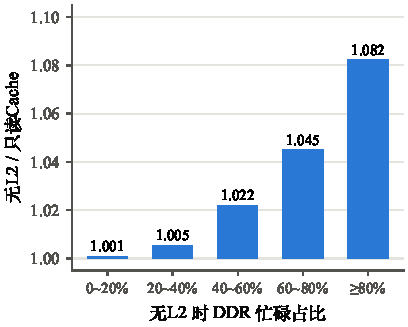
\includegraphics[width=\textwidth]{cache_vs_ddr}
    \caption{同一方案的缓存加速比与无 L2 时 DDR 忙碌占比}
    \label{fig:ddr}
  \end{minipage}\hfill
  \begin{minipage}[t]{0.53\textwidth}
    \centering
    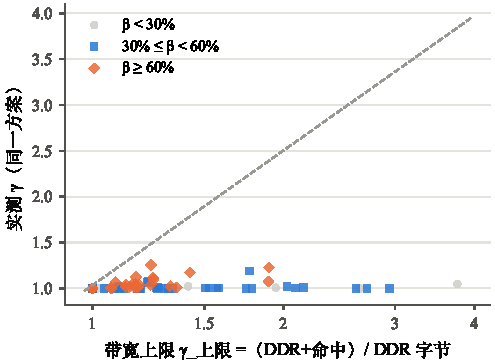
\includegraphics[width=\textwidth]{cache_bound}
    \caption{缓存加速比的实测值与带宽上限 $\bar\gamma$（4 核，最终方案；虚线为 $y=x$）}
    \label{fig:cbound}
  \end{minipage}
\end{figure}

用式 \eqref{eq:miss-class} 对最终方案（4 核）的全部缓存访问做分解（图~\ref{fig:miss}）。按字节计，命中占 \V{fig_miss_hit}，首次缺失占 \V{fig_miss_compulsory}，容量缺失 \V{fig_miss_capacity}，并发缺失 \V{fig_miss_concurrent}。三分之二左右的访问是首次读取，这是计算图决定的上限；在可以争取的部分中，并发缺失与容量缺失量级相当，所以问题三不能只从容量够不够来考虑。

\begin{figure}[H]
  \centering
  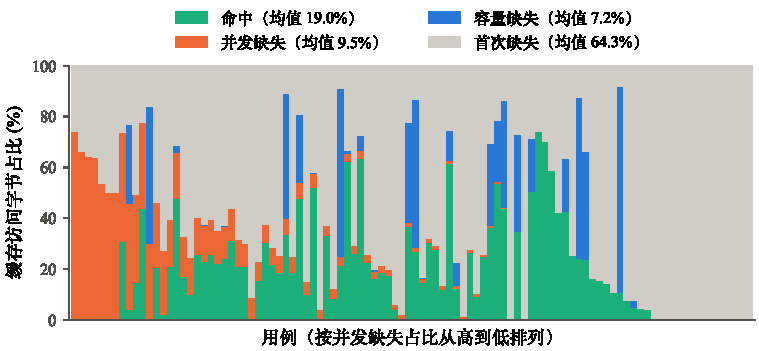
\includegraphics[width=\textwidth]{miss_breakdown}
  \caption{缓存访问的缺失分解（4 核，最终方案，按并发缺失占比从高到低排列）}
  \label{fig:miss}
\end{figure}

图~\ref{fig:p3} 给出 1--5 核下无 L2 与只读 Cache 两种配置的对比曲线和同核数下的缓存加速比，数值汇总在表~\ref{tab:p3-result}，逐用例的 Makespan、总额外搬运量和命中率见附录 C。5 核时只读 Cache 配置的平均加速比为 \V{p3_k5_cache_vs_single}，无 L2 为 \V{p3_k5_noL2_vs_single}；同核数下缓存加速比 $\Gamma_5$ 的均值为 \V{p3_k5_best_mean}，单个用例最高 \V{p3_k5_best_max}。缓存加速比随核数上升（1 核 \V{p3_k1_best_mean}，5 核 \V{p3_k5_best_mean}），命中率也从 \V{p3_k1_hit_mean} 升到 \V{p3_k5_hit_mean}：核数越多，同一张量被越多核心读取，DDR 越紧张，缓存越有用。快速模式下只用 9 个构造候选时，只读 Cache 配置 1--5 核的平均加速比为 \V{figx_fast_p3_k1_mean}、\V{figx_fast_p3_k2_mean}、\V{figx_fast_p3_k3_mean}、\V{figx_fast_p3_k4_mean}、\V{figx_fast_p3_k5_mean}，单个用例同样在数分钟内完成。

\begin{figure}[H]
  \centering
  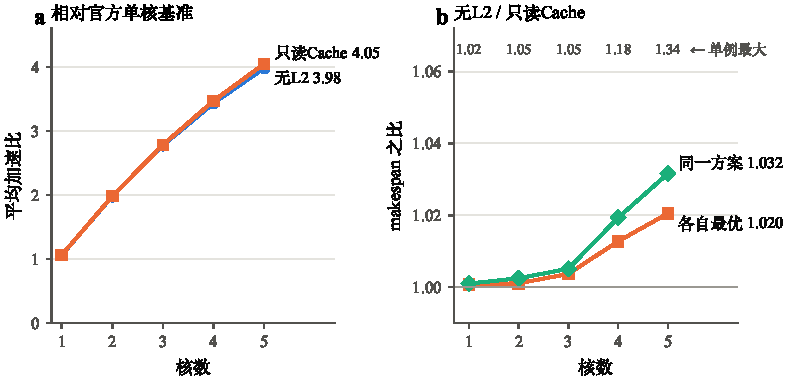
\includegraphics[width=\textwidth]{p3_compare}
  \caption{无 L2 与只读 Cache 两种配置的对比。(a) 两种配置各自逐用例选优后的平均加速比（相对官方单核基准）；(b) 同核数下只读 Cache 相对无 L2 的加速比，“各自最优”为两种配置分别取最优方案，“同一方案”为问题三所选方案放回无 L2 下复评；图顶数字为单例最大值}
  \label{fig:p3}
\end{figure}

\begin{table}[H]
\centering
\caption{问题三结果统计（100 个用例）}
\label{tab:p3-result}
\renewcommand\arraystretch{1.15}
\resizebox{\textwidth}{!}{%
\begin{tabular}{lccccc}
\toprule
 & 1 核 & 2 核 & 3 核 & 4 核 & 5 核 \\
\midrule
无 L2 平均加速比（相对单核基准） & \V{p3_k1_noL2_vs_single} & \V{p3_k2_noL2_vs_single} & \V{p3_k3_noL2_vs_single} & \V{p3_k4_noL2_vs_single} & \V{p3_k5_noL2_vs_single} \\
只读 Cache 平均加速比（相对单核基准） & \V{p3_k1_cache_vs_single} & \V{p3_k2_cache_vs_single} & \V{p3_k3_cache_vs_single} & \V{p3_k4_cache_vs_single} & \V{p3_k5_cache_vs_single} \\
\midrule
缓存加速比 $\Gamma_k$ 均值 & \V{p3_k1_best_mean} & \V{p3_k2_best_mean} & \V{p3_k3_best_mean} & \V{p3_k4_best_mean} & \V{p3_k5_best_mean} \\
\quad 单例最大 & \V{p3_k1_best_max} & \V{p3_k2_best_max} & \V{p3_k3_best_max} & \V{p3_k4_best_max} & \V{p3_k5_best_max} \\
\quad 提升超过 1\% / 5\% 的用例数 & \V{p3_k1_n_gain1pct} / \V{p3_k1_n_gain5pct} & \V{p3_k2_n_gain1pct} / \V{p3_k2_n_gain5pct} & \V{p3_k3_n_gain1pct} / \V{p3_k3_n_gain5pct} & \V{p3_k4_n_gain1pct} / \V{p3_k4_n_gain5pct} & \V{p3_k5_n_gain1pct} / \V{p3_k5_n_gain5pct} \\
同一方案的缓存加速比 $\gamma$ 均值 & \V{p3_k1_same_mean} & \V{p3_k2_same_mean} & \V{p3_k3_same_mean} & \V{p3_k4_same_mean} & \V{p3_k5_same_mean} \\
\midrule
平均命中率 $\theta$ & \V{p3_k1_hit_mean} & \V{p3_k2_hit_mean} & \V{p3_k3_hit_mean} & \V{p3_k4_hit_mean} & \V{p3_k5_hit_mean} \\
平均额外搬运量 / MB（无 L2 / Cache） & \V{p3_k1_noL2_added_MB} / \V{p3_k1_cache_added_MB} & \V{p3_k2_noL2_added_MB} / \V{p3_k2_cache_added_MB} & \V{p3_k3_noL2_added_MB} / \V{p3_k3_cache_added_MB} & \V{p3_k4_noL2_added_MB} / \V{p3_k4_cache_added_MB} & \V{p3_k5_noL2_added_MB} / \V{p3_k5_cache_added_MB} \\
\bottomrule
\end{tabular}}
\end{table}

收益分布很不均匀。5 核时只有 \V{p3_k5_n_gain1pct} 个用例的缓存加速比超过 1.01、\V{p3_k5_n_gain5pct} 个超过 1.05，大多数用例几乎不受影响，它们要么没有被多个核心共享的输入，要么 DDR 本来就不忙。另有 \V{p3_worse_total} 组在“各自最优”口径下缓存反而略慢：\V{p3_worse_list}。两种配置的候选池已经相互复评、完全对称，这 2 组的差距来自缓存对执行时序的扰动（第~\ref{sec:p3-benefit} 节），幅度都在 1.3\% 以内。额外搬运量在只读 Cache 配置下略高于无 L2，这是因为两种配置各自选出的方案不同：只读 Cache 下的最优方案往往把共享张量的消费者分散到更多核心，边界搬运随之增加，但其中一部分由缓存服务，不再占用 DDR 带宽，而题目定义的额外搬运量统计的是 COPY 字节数，不区分数据来自 DDR 还是缓存。后处理方面，问题三中成组合并在 \V{co1_p3_groups} 组里改进了 \V{co1_p3_improved} 组，平均缩短 \V{co1_p3_mean_red_pct}，最多 \V{co1_p3_max_red_pct}；局部搜索起点可追溯的 \V{ls_p3_jobs} 个作业中有 \V{ls_p3_improved} 个改进，平均缩短 \V{ls_p3_mean_red_pct}，改进面比问题一、二广，说明缓存时序对子图顺序的细小变化很敏感。

下面回答题目关于容量和带宽影响的要求。我们固定一批扫描阶段选出的方案，只改变缓存参数重新评估（分析性实验，官方结果仍使用固定配置），结果见图~\ref{fig:sens}。4 核时容量从 256~KB 增至无限，平均 Makespan（相对官方配置）从 \V{fig_sens_k4_cap_ms_0} 降到 \V{fig_sens_k4_cap_ms_6}，命中率从 \V{fig_sens_k4_cap_hit_0} 升到 \V{fig_sens_k4_cap_hit_6}。命中率翻了一倍多，Makespan 只变了约 1\%：增加容量只能消除容量缺失，而容量缺失在全部访问中只占一成左右；多出来的命中又大多发生在 DDR 不忙的用例上，按式 \eqref{eq:ddr-busy} 的分析换不来时间。带宽从 30 升到 60 时，4 核平均 Makespan 从 \V{fig_sens_k4_bw_ms_0} 降到 \V{fig_sens_k4_bw_ms_1}，此后到 1000 几乎不变，因为 250 bytes/cycle 已是 DDR 带宽的 4 倍多，命中读取本身很少成为瓶颈。

\begin{figure}[H]
  \centering
  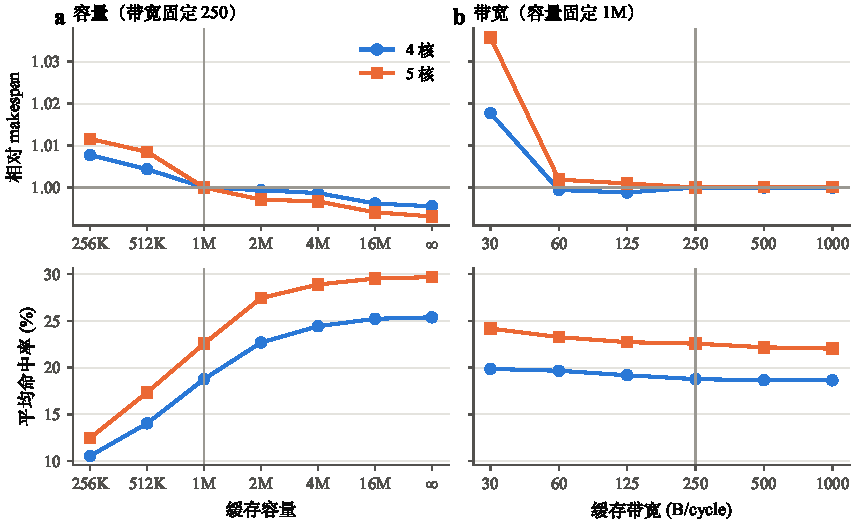
\includegraphics[width=\textwidth]{cache_sensitivity}
  \caption{缓存容量与带宽的敏感性（固定一批扫描阶段方案，只改缓存参数重评；竖线为官方配置）}
  \label{fig:sens}
\end{figure}

由此可以回答题目关于容量和带宽影响切图与调度的问题。在官方配置附近，这批方案对容量和带宽都不敏感，瓶颈不在缓存规格，而在读取的时机和分布。对切图而言，同一张量被越多的核心读取，缓存才越有用武之地，前提是这些读取在时间上错开；对调度而言，关键是让一个核心先把共享张量读进缓存，其他核心随后再读。这一结论来自固定的一批方案，不能直接推广到所有方案。

\label{sec:lockstep}并发缺失的一个典型形态是锁步读取。图~\ref{fig:lockstep} 是 \V{fig_lockstep_case} 在 \V{fig_lockstep_k} 核下一份历史方案的读取时间线（只画被多个核心读取的张量）。在官方配置下，同一张量被几个核心在几十个周期内先后发起读取，第一次读取还没完成，后面的全部未命中，一起挤在 DDR 上；每一轮都是如此，各核像齿轮一样同步推进，命中率只有 \V{fig_lockstep_hit250_pct}，Makespan 为 \V{fig_lockstep_ms250}。把缓存带宽从 250 降到 60 bytes/cycle，同一方案的命中率反而从 \V{fig_lockstep_hit250_pct} 升到 \V{fig_lockstep_hit60_pct}，Makespan 从 \V{fig_lockstep_ms250} 降到 \V{fig_lockstep_ms60}：更慢的缓存打乱了各核的相位，后读的核心晚到一步，恰好落在前一次读取完成之后。这说明在这类用例上，限制缓存收益的是式 \eqref{eq:hit} 中的时序条件，而不是容量条件。降低缓存带宽不是可行方案（配置固定），这个实验只用来确认机理。

\begin{figure}[H]
  \centering
  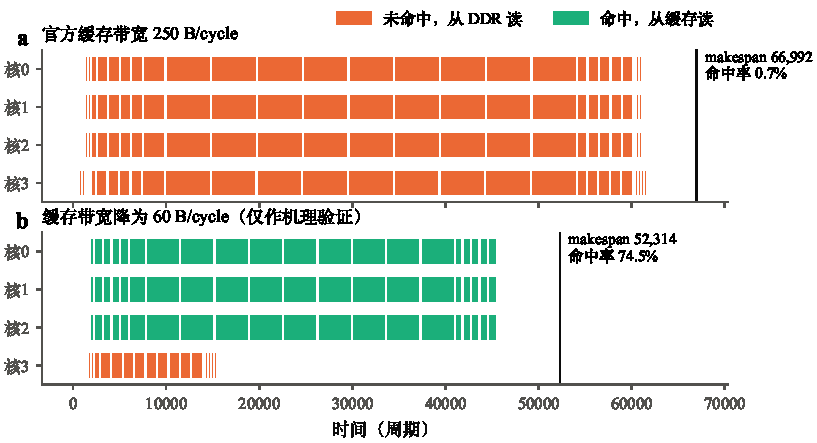
\includegraphics[width=\textwidth]{lockstep}
  \caption{锁步读取（\V{fig_lockstep_case}，\V{fig_lockstep_k} 核，同一份历史方案，只显示被多个核心读取的张量）。(a) 官方缓存带宽；(b) 缓存带宽降为 60 bytes/cycle，仅用于机理验证}
  \label{fig:lockstep}
\end{figure}

最后看两个典型用例。case\_090 在 5 核下的缓存加速比为 \V{cc_case_090_k5_best}，是全部用例中最高的：无 L2 的 Makespan 为 \V{cc_case_090_k5_noL2}，只读 Cache 下为 \V{cc_case_090_k5_cache}，命中率 \V{cc_case_090_k5_hit}。它的 4 核缺失分解中命中占 \V{cc_case_090_k4_share_hit_pct}，首次缺失只有 \V{cc_case_090_k4_share_compulsory_pct}，大量张量被多个核心重复读取，同时并发缺失仍有 \V{cc_case_090_k4_share_concurrent_pct}，若能进一步错开读取还有空间。图~\ref{fig:lockstep} 中的 case\_044 则是另一面：历史方案在问题三下的 Makespan 为 \V{fig_lockstep_ms250}，最终方案降到 \V{cc_case_044_k4_cache}（4 核），同方案缓存加速比为 \V{cc_case_044_k4_same}，命中率 \V{cc_case_044_k4_hit}，但并发缺失仍占 \V{cc_case_044_k4_share_concurrent_pct}，DDR 忙碌占比 \V{cc_case_044_k4_ddrbusy_pct}。最终方案主要靠更好的切图和分核缩短了时间，锁步读取并没有被消除。现有的构造与后处理只能间接改变读取时机，还不能主动控制它，这是本文在缓存利用上的边界。

\section{模型检验与灵敏度分析}

\subsection{结果的可复现性与核数稳定性}\label{sec:repro}

论文和附录中的每一个 Makespan、搬运量和命中率，都来自终版复评：对每个（问题，用例，核数）选出的最优方案，把方案文件重新交给官方评估程序，在固定配置下再评一遍，并要求复评值与选优时记录的值逐位一致。终版复评共 1{,}400 个主结果（问题一 2--5 核、问题二 1--5 核、问题三 1--5 核各 100 个用例）和 500 组问题三同方案配对，全部通过，不一致数为 0。每个方案文件都记录了 SHA-256 哈希，附录中的数字与方案文件、评估输出之间可以逐项核对。

评估过程还跨越了两种运行环境：扫描、成组合并和局部搜索的大部分评估在云服务器（Python 3.10）上完成，终版复评在本机（Python 3.12）上进行，两者记录的 Makespan 逐位一致。这也验证了第 3 节的核内调度确定性假设，逐用例选优的比较是有意义的。

题目要求算法在 2--5 核范围内都能稳定生成高质量结果。经过算法~\ref{alg:select} 的核数补齐，问题一、二、三的全部 100 个用例都满足
\begin{equation}
  M_{k+1}\le M_k,\qquad k=2,3,4\ \ (\text{问题三为 }k=1,\dots,4),
  \label{eq:monotone}
\end{equation}
即多给一个核心，结果不会变差。补齐过程中，问题一、二、三分别评估了 \V{mono_p1}、\V{mono_p2}、\V{mono_p3} 个补空核方案（共 \V{mono_total} 个），经官方评估，其中 \V{mono_identical} 个的 Makespan 与原少核方案相同，没有一例因补空核而改变。

平均并行效率随核数下降（问题一从 2 核的 \V{p1_k2_eff_mean} 降到 5 核的 \V{p1_k5_eff_mean}），这是固定同步延迟和 DDR 共享带宽共同作用的结果，与第~\ref{sec:refs} 节可达参考的变化趋势一致：可达参考的 5 核平均加速比也只有 \V{p1_k5_ref_speedup_mean}（场景 A）和 \V{p2_k5_ref_speedup_mean}（场景 B）。计算图规模对达成率的影响不是简单的越大越好：4 核时达成率与 $\lg$(总计算周期) 的相关系数，问题一只有 \V{p1_k4_size_corr}，问题二为 \V{p2_k4_size_corr}。规模影响的是稳定性（图~\ref{fig:size}）：总计算量低于 $10^5$ 周期的 \V{p1_k4_small_n} 个小图，问题二达成率的标准差为 \V{p2_k4_small_achieve_sd}，$10^6$ 周期以上的大图只有 \V{p2_k4_large_achieve_sd}。小图的结果更依赖具体的依赖链形状，核数补齐也主要在小图上起作用。

\begin{figure}[H]
  \centering
  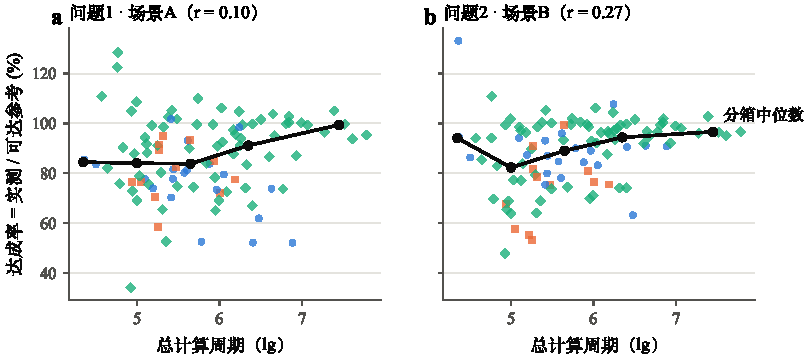
\includegraphics[width=\textwidth]{size_threshold}
  \caption{达成率与规模（4 核）。横轴为总计算周期（对数），折线为分箱中位数}
  \label{fig:size}
\end{figure}

\subsection{各求解环节的贡献}\label{sec:neg-record}

为了检验求解流程中每一步是否必要，我们按来源把候选逐步加入候选池，重新计算三个问题的平均加速比（表~\ref{tab:ladder}）。从朴素基线到三种构造算法逐用例选优，提升最大；成组合并在问题一中把 5 核平均加速比从 \V{ladder_p1_k5_sweep} 提到 \V{ladder_p1_k5_coarsen}，在问题二、三中增量较小；局部搜索、交叉复评和核数补齐每一步的平均增量都不大，但各自在一部分用例上是唯一的改进来源，所以都保留在最终流程中。

\begin{table}[H]
\centering
\caption{按来源逐步加入候选池后的平均加速比（累计；问题三为只读 Cache 配置相对官方单核基准）}
\label{tab:ladder}
\renewcommand\arraystretch{1.15}
\begin{tabular}{lcccccc}
\toprule
\multirow{2}{*}{候选来源} & \multicolumn{2}{c}{问题一} & \multicolumn{2}{c}{问题二} & \multicolumn{2}{c}{问题三} \\
\cmidrule(lr){2-3}\cmidrule(lr){4-5}\cmidrule(lr){6-7}
 & 4 核 & 5 核 & 4 核 & 5 核 & 4 核 & 5 核 \\
\midrule
朴素基线（分量装箱，$\alpha=0.25$） & \V{ladder_p1_k4_naive} & \V{ladder_p1_k5_naive} & \V{ladder_p2_k4_naive} & \V{ladder_p2_k5_naive} & \V{ladder_p3_k4_naive} & \V{ladder_p3_k5_naive} \\
三种构造算法逐用例选优 & \V{ladder_p1_k4_sweep} & \V{ladder_p1_k5_sweep} & \V{ladder_p2_k4_sweep} & \V{ladder_p2_k5_sweep} & \V{ladder_p3_k4_sweep} & \V{ladder_p3_k5_sweep} \\
\quad + 成组合并 & \V{ladder_p1_k4_coarsen} & \V{ladder_p1_k5_coarsen} & \V{ladder_p2_k4_coarsen} & \V{ladder_p2_k5_coarsen} & \V{ladder_p3_k4_coarsen} & \V{ladder_p3_k5_coarsen} \\
\quad + 局部搜索 & \V{ladder_p1_k4_localsearch} & \V{ladder_p1_k5_localsearch} & \V{ladder_p2_k4_localsearch} & \V{ladder_p2_k5_localsearch} & \V{ladder_p3_k4_localsearch} & \V{ladder_p3_k5_localsearch} \\
\quad + 交叉复评（仅问题二、三） & \V{ladder_p1_k4_crosseval} & \V{ladder_p1_k5_crosseval} & \V{ladder_p2_k4_crosseval} & \V{ladder_p2_k5_crosseval} & \V{ladder_p3_k4_crosseval} & \V{ladder_p3_k5_crosseval} \\
\quad + 核数补齐（最终） & \V{ladder_p1_k4_monotone} & \V{ladder_p1_k5_monotone} & \V{ladder_p2_k4_monotone} & \V{ladder_p2_k5_monotone} & \V{ladder_p3_k4_monotone} & \V{ladder_p3_k5_monotone} \\
\bottomrule
\end{tabular}
\end{table}

第~\ref{sec:neg} 节与第~\ref{sec:p3-solve} 节提到的未采用路线，都用当前代码重新运行过，结果文件保存在附件中。错开读取后处理在并发缺失占比最高的 \V{stagger_n} 个用例上（4 核，问题三），与不做错开相比：\V{stagger_better} 例改进（最多 \V{stagger_best_pct}），\V{stagger_same} 例不变，\V{stagger_worse} 例变差（最多变差 \V{stagger_worst_pct}）。这一方向在当前形式下不可用。

\subsection{参数灵敏度}

表~\ref{tab:param} 给出各构造算法在固定参数下的 4 核平均加速比（只列覆盖全部 100 个用例的参数值）。分量装箱的 $\alpha$ 越大越差，$\alpha\le 0.25$ 时分量不被切开，结果相同，说明对多分量图把整个分量放在一起几乎总是对的。层带划分的最优方向在两个场景下相反：问题一中 $W=16$（粗切）最好，问题二中 $W=4096$（细切）最好，这正是第~\ref{sec:p1-model} 节和第~\ref{sec:p2-model} 节的模型所预测的：场景 A 中路径上的子图边界是代价，场景 B 中只有换核才是。任何固定参数的平均值都明显低于逐用例选优（4 核问题一 \V{p1_k4_portfolio_mean}、问题二 \V{p2_k4_portfolio_mean}），而同一算法内逐用例调参的收益很小（例如分量装箱从固定 $\alpha=0.25$ 的 \V{sens_p1_lpt_0p25} 到逐用例最优的 \V{p1_k4_lpt_mean}）。对这批用例，选对构造算法比在同一算法内调参重要得多。

\begin{table}[H]
\centering
\caption{构造算法在固定参数下的 4 核平均加速比}
\label{tab:param}
\renewcommand\arraystretch{1.15}
\begin{tabular}{llcc}
\toprule
算法 & 参数取值 & 问题一 & 问题二 \\
\midrule
\multirow{7}{*}{分量装箱 $\alpha$}
 & 0.1 & \V{sens_p1_lpt_0p1} & \V{sens_p2_lpt_0p1} \\
 & 0.25 & \V{sens_p1_lpt_0p25} & \V{sens_p2_lpt_0p25} \\
 & 0.5 & \V{sens_p1_lpt_0p5} & \V{sens_p2_lpt_0p5} \\
 & 1 & \V{sens_p1_lpt_1} & \V{sens_p2_lpt_1} \\
 & 2 & \V{sens_p1_lpt_2} & \V{sens_p2_lpt_2} \\
 & 4 & \V{sens_p1_lpt_4} & \V{sens_p2_lpt_4} \\
 & 8 & \V{sens_p1_lpt_8} & \V{sens_p2_lpt_8} \\
\midrule
\multirow{3}{*}{层带划分 $W$}
 & 16 & \V{sens_p1_band_16} & \V{sens_p2_band_16} \\
 & 256 & \V{sens_p1_band_256} & \V{sens_p2_band_256} \\
 & 4096 & \V{sens_p1_band_4096} & \V{sens_p2_band_4096} \\
\midrule
\multirow{3}{*}{相位构造 $\lambda$}
 & 2000 & \V{sens_p1_phase_2000} & \V{sens_p2_phase_2000} \\
 & $10^4$ & \V{sens_p1_phase_10000} & \V{sens_p2_phase_10000} \\
 & $5\times10^4$ & \V{sens_p1_phase_50000} & \V{sens_p2_phase_50000} \\
\bottomrule
\end{tabular}
\end{table}

\subsection{硬件参数扰动下的鲁棒性}

官方配置是固定的，但实际硬件的带宽和同步开销会有波动。我们检验本文方案的优势是否依赖于某个具体参数：从三类中各取 10 个用例（按编号等间隔抽取），在 4 核下把 DDR 带宽改为 48、72 bytes/cycle（$\pm20\%$），或把同步相关的等待与延迟同时乘以 0.8、1.2，分别评估本文的最终方案和朴素方案（分量装箱，$\alpha=0.25$）。注意本文方案是在官方配置下选出的，扰动后没有重新优化。结果见表~\ref{tab:robust}。

\begin{table}[H]
\centering
\caption{参数扰动下本文方案相对朴素方案的 Makespan 比（几何平均，大于 1 表示本文更快；4 核，\V{rob_p1_official_n} 个用例）}
\label{tab:robust}
\renewcommand\arraystretch{1.15}
\begin{tabular}{lcccc}
\toprule
\multirow{2}{*}{配置} & \multicolumn{2}{c}{问题一} & \multicolumn{2}{c}{问题二} \\
\cmidrule(lr){2-3}\cmidrule(lr){4-5}
 & 朴素 / 本文 & 本文方案 Makespan 变化 & 朴素 / 本文 & 本文方案 Makespan 变化 \\
\midrule
官方配置 & \V{rob_p1_official_adv} & 1.00 & \V{rob_p2_official_adv} & 1.00 \\
DDR 带宽 48 & \V{rob_p1_bw48_adv} & \V{rob_p1_bw48_ms_ratio} & \V{rob_p2_bw48_adv} & \V{rob_p2_bw48_ms_ratio} \\
DDR 带宽 72 & \V{rob_p1_bw72_adv} & \V{rob_p1_bw72_ms_ratio} & \V{rob_p2_bw72_adv} & \V{rob_p2_bw72_ms_ratio} \\
同步开销 $\times 0.8$ & \V{rob_p1_sync08_adv} & \V{rob_p1_sync08_ms_ratio} & \V{rob_p2_sync08_adv} & \V{rob_p2_sync08_ms_ratio} \\
同步开销 $\times 1.2$ & \V{rob_p1_sync12_adv} & \V{rob_p1_sync12_ms_ratio} & \V{rob_p2_sync12_adv} & \V{rob_p2_sync12_ms_ratio} \\
\bottomrule
\end{tabular}
\end{table}

四种扰动下，本文方案相对朴素方案的优势基本不变：问题一保持在 \V{rob_p1_sync12_adv}--\V{rob_p1_sync08_adv} 倍、问题二保持在 \V{rob_p2_bw48_adv}--\V{rob_p2_sync08_adv} 倍。逐用例看，只有问题二带宽降为 48 时有 \V{rob_p2_bw48_nworse} 个用例本文方案略慢于朴素方案（比值 \V{rob_p2_bw48_minadv}），其余配置下没有一例反超。本文方案自身的 Makespan 随带宽下降而增加、随同步开销增加而增加，方向与模型一致，幅度都在 3\% 以内。这说明方案的优势来自结构性的切分方式，而不是对某组参数的过拟合。

\subsection{运行时间}

三种构造算法本身都很快。在本机（负载较高时）单进程测量，4 核方案的生成时间中位数为：分量装箱 \V{time_lpt_median} 秒、层带划分 \V{time_band_median} 秒、相位构造 \V{time_phase_median} 秒；最大的用例 \V{time_bigcase}（\V{time_bigcase_ops} 个操作）上最慢的一次也只需 \V{time_all_max} 秒。耗时主要在官方评估程序上。题目要求单个用例以 5--10 分钟内给出结果为佳，我们在最大用例上实测了附件程序的快速模式（9 个构造候选加 21 个成组合并变体，共 30 次官方评估）：CPU 时间合计约 \V{figx_fast_big_cpu_min} 分钟，8 进程并行时墙钟时间约 1 分钟。快速模式的求解质量见第 5.4.2、5.7.2 与 5.10.2 节，仅用 9 个构造候选时，5 核平均加速比已达最终结果的 90\%--96\%。由局部搜索的记录推算，单次评估的中位数为 \V{eval_secs_median} 秒，最大的用例上约 \V{eval_secs_max} 秒。

附件程序只依赖 Python 3.10 及以上版本的标准库和赛题官方材料包，提供两种运行方式。求解入口 \texttt{solve.py} 对给定计算图与核数运行三种构造算法（各 3 组代表参数）和成组合并，由官方评估程序选出最优方案，单个用例一般在数分钟内完成；复现入口 \texttt{reproduce.py} 读取本文的 1{,}400 个最终方案文件并调用官方评估程序，逐项复现附录中的数字。三种构造算法分别实现在 \texttt{nmcs/algos.py}、\texttt{algos2.py}、\texttt{algos4.py} 中，参数扫描、后处理与统计作图的完整实验代码在 \texttt{research\_code/} 目录下。

\section{模型的评价与推广}

\subsection{主要结论}

对问题一，场景 A 的代价由依赖路径上的子图边界决定：每个边界带来一次 DDR 往返和 100 或 1000 周期的激活等待，并沿路径线性累积（命题~\ref{prop:path}）。据此设计的三种构造算法分别适合多分量、单一巨块和汇聚链结构，合法性由命题~\ref{prop:acyclic} 保证；逐用例选优与成组合并贡献了主要提升，核数补齐保证了 2--5 核结果单调。最终 5 核平均加速比为 \V{p1_k5_final_mean}，对含同步可达参考的达成率为 \V{p1_k5_achieve_mean}，剩余差距集中在 I 类小图上，受场景 A 固定延迟所限。

对问题二，同核子图合并为一个 Task 后，边界搬运由子图边界变为核边界（命题~\ref{prop:qb}），时间代价只随换核次数累积（式 \eqref{eq:path-B}），模型因此预测场景 B 适合细分，扫描数据与之一致。另一方面，跨子图的驻留数据加重了缓存压力（式 \eqref{eq:resident}），少数用例因此不如场景 A。最终 5 核平均加速比为 \V{p2_k5_final_mean}，I 类从问题一的 \V{p1_k5_famI_mean} 提高到 \V{p2_k5_famI_mean}。

对问题三，只读 L2 Cache 的命中同时受时序条件与容量条件约束（式 \eqref{eq:hit}），命中能否换来时间还取决于 DDR 是否紧张（式 \eqref{eq:ddr-busy}、\eqref{eq:gamma-bound}）。在官方配置附近，限制缓存收益的主要是读取时序而不是容量和带宽，锁步读取的对照实验提供了直接证据。两问共享候选池后，5 核只读 Cache 配置的平均加速比为 \V{p3_k5_cache_vs_single}，同核数缓存加速比为 \V{p3_k5_best_mean}，单例最高 \V{p3_k5_best_max}。

\subsection{模型的优点}

合法性由构造保证。三种构造算法都给子图一个随依赖严格递增的编号，生成的方案不需要事后修补就能通过评估程序的检查；后处理中可能成环的成组合并候选由评估程序检查后丢弃，不影响最终结果的合法性。

结果有参照，差距可以量化。第~\ref{sec:refs} 节的解析下界、零通信表调度和含同步可达参考逐步收紧，解析下界在 400 组（用例，核数）的实测中从未被突破。每个结果都能说明离可达水平还差多少，而不只是相对自身基线的提升。

模型能解释实验现象。命题~\ref{prop:path} 解释了场景 A 中为什么代价取决于路径深度，命题~\ref{prop:qb} 与式 \eqref{eq:path-B} 解释了场景 B 为什么适合细分，式 \eqref{eq:resident} 解释了少数用例场景 B 不如场景 A，式 \eqref{eq:hit} 与式 \eqref{eq:ddr-busy} 解释了只读 Cache 收益为什么小而集中。参数灵敏度中层带划分在两个场景下方向相反（表~\ref{tab:param}），也与模型的预测一致。全部数字来自官方评估程序的终版复评，1{,}400 个主结果逐位一致，三个问题都满足核数单调，未采用的路线也保留了可重现的实验记录。

\subsection{模型的不足}

简化模型只是松弛。式 \eqref{eq:obj-p1}、\eqref{eq:obj-p2} 忽略了 DDR 带宽争用和核内换出，它的最优解不一定是评估程序下的最优解，所以我们只用它指导算法设计和给出参照，最终结果依赖评估程序选优。含同步可达参考也只是贪心结果，4 核时问题一有 \V{p1_k4_above_ref} 个、问题二有 \V{p2_k4_above_ref} 个用例的实测值超过了它。

I 类中的小图仍是短板。5 核时 I 类的平均加速比，问题一为 \V{p1_k5_famI_mean}、问题二为 \V{p2_k5_famI_mean}，对可达参考的达成率为 \V{p1_k5_famI_achieve} 和 \V{p2_k5_famI_achieve}，低于 III 类（\V{p1_k5_famIII_achieve}、\V{p2_k5_famIII_achieve}）。对单核基准只有两万周期左右的小图，场景 A 的 1000 周期跨核等待使任何切分都得不偿失。

缓存的潜力没有充分挖掘，搜索成本也偏高。问题三 5 核的平均缓存加速比只有 \V{p3_k5_best_mean}，我们找到了限制收益的机理，但主动安排读取错位的两种尝试都没有成功。局部搜索用掉了 \V{ls_tries_total} 次官方评估，占全部 \V{evals_total} 次评估的 \V{ls_share_pct}，平均改进在几个百分点以内；更经济的做法可能是先用式 \eqref{eq:task-dur} 这类快速估计预筛候选，只把最有希望的交给评估程序。

\subsection{模型的推广}

三种构造算法的复杂度对核数是线性的，可以直接用于核数更多的 NPU。核数增加后，跨核同步在关键路径上的占比会继续上升，相位构造中的 $\lambda$ 和核数补齐会更重要。在实际编译器中，本文的结构分类与逐用例选优可以作为切图策略的选择器：先用 $\eta$、$\omega$ 等静态特征判断计算图类型，再决定用哪种构造算法，不必对每张图做完整搜索。

在缓存感知调度方面，式 \eqref{eq:hit} 给出了命中的时序条件。若能在调度阶段为每个共享张量指定领读核心，让跟读核心的 COPY\_IN 晚于领读完成时刻，就能把并发缺失转化为命中。第~\ref{sec:lockstep} 节的锁步实验表明，在部分用例上这样做的收益可能达到两成以上，这是值得继续研究的方向。


% 参考文献：按正文首次引用顺序排列；格式按附件2（期刊：作者，论文名，杂志名，卷期号：起止页码，出版年）
\begin{thebibliography}{99}
\bibitem{liao2019davinci} H. Liao, J. Tu, J. Xia, X. Zhou，DaVinci: A scalable architecture for neural network computing，2019 IEEE Hot Chips 31 Symposium (HCS)：1--44，2019。
\bibitem{kwok1999static} Y.-K. Kwok, I. Ahmad，Static scheduling algorithms for allocating directed task graphs to multiprocessors，ACM Computing Surveys，31(4)：406--471，1999。
\bibitem{garey1978strong} M. R. Garey, D. S. Johnson，``Strong'' NP-completeness results: motivation, examples, and implications，Journal of the ACM，25(3)：499--508，1978。
\bibitem{herrmann2019acyclic} J. Herrmann, M. Y. Özkaya, B. Uçar, K. Kaya, Ü. V. Çatalyürek，Multilevel algorithms for acyclic partitioning of directed acyclic graphs，SIAM Journal on Scientific Computing，41(4)：A2117--A2145，2019。
\bibitem{graham1969bounds} R. L. Graham，Bounds on multiprocessing timing anomalies，SIAM Journal on Applied Mathematics，17(2)：416--429，1969。
\bibitem{topcuoglu2002performance} H. Topcuoglu, S. Hariri, M.-Y. Wu，Performance-effective and low-complexity task scheduling for heterogeneous computing，IEEE Transactions on Parallel and Distributed Systems，13(3)：260--274，2002。
\bibitem{belady1966study} L. A. Belady，A study of replacement algorithms for a virtual-storage computer，IBM Systems Journal，5(2)：78--101，1966。
\bibitem{hill1989evaluating} M. D. Hill, A. J. Smith，Evaluating associativity in CPU caches，IEEE Transactions on Computers，38(12)：1612--1630，1989。
\end{thebibliography}



\begin{appendices}
\section{问题一逐用例结果}
\begin{footnotesize}
\setlength{\tabcolsep}{2.6pt}
\begin{longtable}{l r rr rr rr rr}
\caption{问题一逐用例结果：Makespan（周期）与总额外搬运量（字节）}\label{tab:app-p1}\\
\toprule
\multirow{2}{*}{用例} & \multirow{2}{*}{单核基准} & \multicolumn{2}{c}{2 核} & \multicolumn{2}{c}{3 核} & \multicolumn{2}{c}{4 核} & \multicolumn{2}{c}{5 核} \\
\cmidrule(lr){3-4}\cmidrule(lr){5-6}\cmidrule(lr){7-8}\cmidrule(lr){9-10}
 & & Makespan & 额外搬运 & Makespan & 额外搬运 & Makespan & 额外搬运 & Makespan & 额外搬运 \\
\midrule
\endfirsthead
\toprule
用例 & 单核基准 & \multicolumn{2}{c}{2 核} & \multicolumn{2}{c}{3 核} & \multicolumn{2}{c}{4 核} & \multicolumn{2}{c}{5 核} \\
\midrule
\endhead
\bottomrule
\endfoot
case\_001 & 233{,}110 & 116{,}868 & 1{,}152 & 93{,}135 & 862{,}464 & 58{,}984 & 3{,}456 & 47{,}502 & 4{,}608 \\
case\_002 & 261{,}945 & 133{,}944 & 5{,}165{,}568 & 101{,}425 & 964{,}608 & 77{,}554 & 766{,}464 & 65{,}085 & 910{,}848 \\
case\_003 & 602{,}212 & 372{,}446 & 6{,}590{,}892 & 280{,}827 & 7{,}330{,}768 & 267{,}227 & 8{,}010{,}228 & 256{,}255 & 8{,}971{,}928 \\
case\_004 & 392{,}357 & 213{,}333 & 4{,}306{,}944 & 134{,}043 & 221{,}184 & 108{,}126 & 3{,}741{,}696 & 95{,}289 & 3{,}852{,}288 \\
case\_005 & 95{,}618 & 74{,}654 & 2{,}341{,}728 & 67{,}164 & 2{,}443{,}372 & 67{,}076 & 2{,}693{,}956 & 67{,}076 & 2{,}693{,}956 \\
case\_006 & 82{,}837 & 39{,}720 & 39{,}190 & 30{,}961 & 94{,}344 & 30{,}961 & 94{,}344 & 30{,}961 & 94{,}344 \\
case\_007 & 1{,}012{,}562 & 579{,}668 & 11{,}993{,}088 & 338{,}094 & 55{,}296 & 338{,}094 & 55{,}296 & 203{,}834 & 110{,}592 \\
case\_008 & 487{,}605 & 244{,}266 & 0 & 163{,}359 & 0 & 123{,}060 & 0 & 100{,}603 & 0 \\
case\_009 & 153{,}261 & 92{,}198 & 172{,}032 & 92{,}198 & 172{,}032 & 92{,}198 & 172{,}032 & 92{,}198 & 172{,}032 \\
case\_010 & 86{,}969 & 45{,}272 & 48{,}384 & 33{,}937 & 836{,}616 & 29{,}586 & 362{,}880 & 29{,}586 & 362{,}880 \\
case\_011 & 184{,}697 & 92{,}646 & 180{,}224 & 69{,}625 & 1{,}081{,}344 & 46{,}880 & 540{,}672 & 46{,}880 & 540{,}672 \\
case\_012 & 59{,}088 & 30{,}094 & 28{,}800 & 21{,}894 & 20{,}160 & 17{,}253 & 39{,}168 & 14{,}300 & 49{,}536 \\
case\_013 & 263{,}949 & 132{,}198 & 8{,}192 & 88{,}351 & 16{,}384 & 66{,}982 & 24{,}576 & 54{,}363 & 32{,}768 \\
case\_014 & 17{,}698{,}626 & 8{,}813{,}761 & 81{,}618{,}360 & 5{,}934{,}584 & 81{,}312{,}936 & 4{,}512{,}560 & 94{,}384{,}536 & 3{,}677{,}086 & 86{,}530{,}056 \\
case\_015 & 177{,}362 & 92{,}411 & 224{,}536 & 60{,}766 & 278{,}280 & 54{,}989 & 528{,}396 & 41{,}506 & 317{,}952 \\
case\_016 & 7{,}715{,}523 & 7{,}704{,}912 & 393{,}264 & 6{,}868{,}180 & 119{,}561{,}444 & 5{,}445{,}426 & 119{,}559{,}028 & 5{,}445{,}426 & 119{,}559{,}028 \\
case\_017 & 162{,}810 & 75{,}539 & 92{,}160 & 59{,}088 & 179{,}712 & 39{,}520 & 263{,}808 & 34{,}720 & 347{,}904 \\
case\_018 & 1{,}004{,}367 & 507{,}450 & 2{,}896{,}896 & 348{,}029 & 4{,}182{,}400 & 267{,}407 & 5{,}185{,}280 & 213{,}703 & 5{,}586{,}304 \\
case\_019 & 81{,}144 & 43{,}224 & 27{,}168 & 29{,}062 & 27{,}168 & 24{,}031 & 256{,}128 & 19{,}200 & 94{,}848 \\
case\_020 & 532{,}746 & 266{,}580 & 0 & 177{,}950 & 0 & 133{,}704 & 0 & 107{,}650 & 0 \\
case\_021 & 6{,}567{,}937 & 3{,}112{,}600 & 8{,}908{,}800 & 2{,}096{,}552 & 12{,}902{,}400 & 1{,}550{,}324 & 4{,}608{,}000 & 1{,}243{,}902 & 13{,}516{,}800 \\
case\_022 & 56{,}780 & 28{,}333 & 6{,}912 & 19{,}053 & 13{,}824 & 14{,}654 & 13{,}824 & 11{,}828 & 20{,}736 \\
case\_023 & 122{,}614 & 63{,}076 & 122{,}936 & 41{,}662 & 196{,}896 & 31{,}083 & 281{,}280 & 24{,}947 & 270{,}912 \\
case\_024 & 2{,}555{,}343 & 2{,}544{,}732 & 393{,}264 & 2{,}267{,}368 & 39{,}329{,}468 & 1{,}799{,}130 & 39{,}328{,}684 & 1{,}799{,}130 & 39{,}328{,}684 \\
case\_025 & 4{,}863{,}026 & 2{,}431{,}840 & 27{,}648 & 1{,}626{,}688 & 552{,}960 & 1{,}596{,}420 & 57{,}474{,}048 & 1{,}364{,}832 & 57{,}830{,}400 \\
case\_026 & 99{,}203 & 62{,}589 & 606{,}260 & 41{,}187 & 217{,}872 & 41{,}187 & 217{,}872 & 41{,}187 & 217{,}872 \\
case\_027 & 2{,}363{,}952 & 1{,}116{,}984 & 1{,}843{,}200 & 837{,}049 & 3{,}686{,}400 & 559{,}196 & 3{,}317{,}760 & 558{,}753 & 5{,}529{,}600 \\
case\_028 & 43{,}836{,}040 & 20{,}572{,}367 & 48{,}637{,}056 & 13{,}753{,}608 & 48{,}529{,}152 & 10{,}408{,}288 & 48{,}817{,}536 & 8{,}372{,}068 & 50{,}895{,}360 \\
case\_029 & 37{,}555 & 19{,}740 & 0 & 12{,}743 & 0 & 11{,}028 & 0 & 9{,}383 & 0 \\
case\_030 & 2{,}808{,}034 & 1{,}396{,}845 & 9{,}431{,}040 & 932{,}172 & 9{,}679{,}360 & 698{,}521 & 7{,}334{,}912 & 560{,}819 & 10{,}660{,}864 \\
case\_031 & 1{,}414{,}369 & 733{,}667 & 6{,}908{,}928 & 485{,}282 & 4{,}462{,}080 & 390{,}234 & 8{,}598{,}820 & 307{,}352 & 8{,}056{,}320 \\
case\_032 & 41{,}443 & 21{,}771 & 18{,}504 & 15{,}388 & 18{,}504 & 14{,}942 & 92{,}316 & 10{,}220 & 24{,}648 \\
case\_033 & 1{,}774{,}196 & 886{,}462 & 6{,}188{,}064 & 601{,}413 & 9{,}595{,}488 & 453{,}651 & 9{,}513{,}600 & 367{,}551 & 8{,}062{,}080 \\
case\_034 & 842{,}996 & 417{,}250 & 1{,}620{,}992 & 276{,}682 & 2{,}939{,}392 & 212{,}296 & 3{,}256{,}832 & 177{,}825 & 3{,}567{,}616 \\
case\_035 & 169{,}571 & 95{,}406 & 9{,}216 & 95{,}406 & 9{,}216 & 95{,}406 & 9{,}216 & 95{,}406 & 9{,}216 \\
case\_036 & 931{,}510 & 466{,}068 & 1{,}152 & 458{,}829 & 8{,}751{,}360 & 233{,}584 & 3{,}456 & 187{,}182 & 4{,}608 \\
case\_037 & 210{,}001 & 105{,}374 & 204{,}800 & 74{,}038 & 1{,}064{,}960 & 53{,}320 & 614{,}400 & 43{,}800 & 1{,}925{,}120 \\
case\_038 & 1{,}364{,}555 & 679{,}403 & 4{,}979{,}712 & 455{,}753 & 6{,}337{,}536 & 344{,}959 & 7{,}661{,}056 & 286{,}350 & 8{,}475{,}648 \\
case\_039 & 1{,}435{,}262 & 692{,}660 & 13{,}541{,}376 & 480{,}930 & 15{,}622{,}144 & 395{,}323 & 17{,}604{,}608 & 395{,}323 & 17{,}604{,}608 \\
case\_040 & 253{,}454 & 126{,}251 & 115{,}200 & 110{,}105 & 316{,}416 & 110{,}105 & 316{,}416 & 110{,}105 & 545{,}800 \\
case\_041 & 6{,}003{,}957 & 2{,}970{,}011 & 36{,}372{,}480 & 1{,}984{,}030 & 40{,}424{,}448 & 1{,}490{,}758 & 36{,}624{,}384 & 1{,}196{,}239 & 39{,}533{,}568 \\
case\_042 & 1{,}686{,}740 & 842{,}181 & 6{,}817{,}056 & 584{,}180 & 8{,}561{,}952 & 433{,}784 & 10{,}958{,}976 & 359{,}815 & 11{,}529{,}504 \\
case\_043 & 677{,}656 & 340{,}574 & 737{,}280 & 268{,}448 & 2{,}257{,}920 & 268{,}172 & 2{,}398{,}342 & 268{,}172 & 2{,}398{,}342 \\
case\_044 & 154{,}407 & 61{,}545 & 1{,}395{,}040 & 61{,}545 & 1{,}395{,}040 & 61{,}545 & 1{,}395{,}040 & 61{,}545 & 1{,}395{,}040 \\
case\_045 & 125{,}614 & 69{,}275 & 368{,}640 & 45{,}572 & 0 & 33{,}246 & 0 & 29{,}135 & 0 \\
case\_046 & 276{,}455 & 128{,}056 & 1{,}192{,}544 & 102{,}504 & 2{,}321{,}600 & 102{,}504 & 2{,}321{,}600 & 102{,}504 & 2{,}321{,}600 \\
case\_047 & 326{,}508 & 237{,}888 & 2{,}548{,}464 & 203{,}634 & 2{,}716{,}176 & 186{,}124 & 2{,}918{,}704 & 178{,}918 & 3{,}102{,}288 \\
case\_048 & 222{,}220 & 149{,}315 & 1{,}043{,}010 & 135{,}083 & 1{,}107{,}632 & 135{,}083 & 1{,}107{,}632 & 135{,}083 & 1{,}107{,}632 \\
case\_049 & 196{,}276 & 147{,}531 & 2{,}868{,}130 & 131{,}522 & 2{,}981{,}982 & 122{,}133 & 2{,}962{,}918 & 122{,}133 & 2{,}962{,}918 \\
case\_050 & 149{,}690 & 106{,}870 & 74{,}860 & 96{,}346 & 2{,}723{,}246 & 89{,}427 & 2{,}725{,}404 & 89{,}427 & 2{,}725{,}404 \\
case\_051 & 607{,}628 & 558{,}663 & 21{,}627{,}306 & 436{,}197 & 11{,}273{,}748 & 422{,}863 & 9{,}045{,}668 & 422{,}863 & 9{,}045{,}668 \\
case\_052 & 180{,}301 & 101{,}771 & 2{,}663{,}284 & 81{,}151 & 2{,}057{,}578 & 61{,}662 & 407{,}040 & 50{,}807 & 443{,}904 \\
case\_053 & 1{,}472{,}686 & 725{,}195 & 10{,}517{,}152 & 539{,}122 & 6{,}888{,}192 & 492{,}232 & 11{,}271{,}680 & 484{,}927 & 11{,}937{,}528 \\
case\_054 & 815{,}051 & 517{,}960 & 1{,}130{,}496 & 457{,}565 & 11{,}226{,}296 & 405{,}511 & 11{,}493{,}906 & 376{,}524 & 11{,}981{,}934 \\
case\_055 & 118{,}835 & 56{,}840 & 99{,}328 & 38{,}542 & 115{,}712 & 35{,}590 & 243{,}724 & 26{,}469 & 198{,}656 \\
case\_056 & 277{,}285 & 215{,}107 & 2{,}685{,}186 & 186{,}802 & 3{,}021{,}450 & 175{,}720 & 3{,}035{,}580 & 166{,}663 & 3{,}074{,}222 \\
case\_057 & 59{,}726 & 33{,}702 & 93{,}988 & 25{,}250 & 14{,}112 & 20{,}957 & 14{,}112 & 16{,}502 & 69{,}696 \\
case\_058 & 4{,}539{,}717 & 2{,}193{,}367 & 38{,}522{,}880 & 1{,}526{,}970 & 56{,}279{,}040 & 1{,}145{,}057 & 47{,}173{,}632 & 1{,}004{,}819 & 32{,}104{,}448 \\
case\_059 & 829{,}473 & 369{,}318 & 360{,}448 & 255{,}117 & 6{,}352{,}896 & 185{,}216 & 1{,}081{,}344 & 150{,}736 & 4{,}866{,}048 \\
case\_060 & 888{,}789 & 471{,}857 & 3{,}890{,}320 & 340{,}707 & 3{,}736{,}840 & 291{,}315 & 3{,}973{,}392 & 249{,}327 & 4{,}516{,}232 \\
case\_061 & 77{,}191 & 55{,}396 & 1{,}162{,}876 & 43{,}481 & 1{,}265{,}444 & 23{,}455 & 64{,}512 & 22{,}283 & 182{,}784 \\
case\_062 & 2{,}854{,}809 & 1{,}417{,}218 & 58{,}354{,}176 & 1{,}079{,}181 & 10{,}572{,}288 & 1{,}079{,}181 & 10{,}572{,}288 & 1{,}079{,}181 & 10{,}572{,}288 \\
case\_063 & 1{,}070{,}397 & 529{,}854 & 21{,}474{,}816 & 413{,}784 & 4{,}399{,}104 & 316{,}530 & 3{,}806{,}208 & 259{,}997 & 3{,}757{,}056 \\
case\_064 & 19{,}116 & 16{,}926 & 81{,}696 & 16{,}926 & 81{,}696 & 16{,}926 & 81{,}696 & 16{,}926 & 81{,}696 \\
case\_065 & 53{,}068 & 26{,}233 & 14{,}112 & 18{,}001 & 27{,}936 & 14{,}178 & 41{,}904 & 12{,}169 & 55{,}584 \\
case\_066 & 359{,}070 & 207{,}194 & 3{,}560{,}460 & 154{,}448 & 3{,}843{,}658 & 143{,}175 & 4{,}313{,}164 & 132{,}051 & 4{,}607{,}842 \\
case\_067 & 63{,}834{,}834 & 30{,}462{,}883 & 74{,}951{,}040 & 20{,}430{,}262 & 77{,}820{,}672 & 15{,}482{,}490 & 81{,}542{,}272 & 12{,}751{,}707 & 90{,}050{,}048 \\
case\_068 & 362{,}095 & 227{,}799 & 2{,}740{,}574 & 187{,}938 & 3{,}674{,}512 & 169{,}482 & 3{,}735{,}730 & 168{,}776 & 3{,}808{,}662 \\
case\_069 & 25{,}144 & 25{,}111 & 68{,}740 & 21{,}307 & 426{,}484 & 19{,}837 & 386{,}908 & 19{,}038 & 552{,}942 \\
case\_070 & 117{,}300 & 70{,}357 & 700{,}584 & 41{,}299 & 273{,}408 & 41{,}299 & 273{,}408 & 30{,}598 & 462{,}848 \\
case\_071 & 18{,}919 & 18{,}919 & 0 & 15{,}923 & 350{,}698 & 14{,}867 & 353{,}802 & 14{,}757 & 343{,}264 \\
case\_072 & 23{,}897{,}828 & 11{,}619{,}091 & 116{,}910{,}880 & 7{,}842{,}498 & 121{,}621{,}280 & 5{,}885{,}034 & 124{,}709{,}664 & 4{,}788{,}636 & 129{,}778{,}352 \\
case\_073 & 10{,}081{,}626 & 4{,}344{,}547 & 16{,}800{,}640 & 2{,}967{,}238 & 19{,}443{,}968 & 2{,}356{,}726 & 20{,}829{,}312 & 2{,}005{,}012 & 24{,}550{,}912 \\
case\_074 & 1{,}682{,}239 & 817{,}481 & 7{,}168{,}000 & 545{,}581 & 8{,}437{,}760 & 437{,}729 & 13{,}484{,}036 & 335{,}235 & 11{,}317{,}248 \\
case\_075 & 1{,}441{,}809 & 824{,}894 & 8{,}622{,}006 & 686{,}606 & 10{,}055{,}794 & 507{,}973 & 10{,}511{,}278 & 465{,}714 & 11{,}274{,}346 \\
case\_076 & 6{,}185{,}113 & 3{,}044{,}060 & 42{,}184{,}704 & 2{,}034{,}436 & 42{,}454{,}016 & 1{,}523{,}743 & 42{,}636{,}288 & 1{,}228{,}370 & 36{,}692{,}992 \\
case\_077 & 495{,}320 & 249{,}892 & 57{,}344 & 177{,}805 & 114{,}688 & 145{,}044 & 172{,}032 & 120{,}238 & 172{,}032 \\
case\_078 & 2{,}296{,}143 & 1{,}080{,}972 & 15{,}039{,}360 & 840{,}164 & 6{,}508{,}800 & 619{,}540 & 15{,}039{,}360 & 605{,}119 & 10{,}578{,}432 \\
case\_079 & 31{,}052{,}251 & 14{,}734{,}808 & 40{,}415{,}232 & 9{,}817{,}862 & 44{,}064{,}768 & 7{,}392{,}284 & 47{,}714{,}304 & 5{,}933{,}675 & 59{,}271{,}168 \\
case\_080 & 292{,}138 & 145{,}926 & 2{,}191{,}360 & 100{,}325 & 3{,}047{,}424 & 100{,}325 & 3{,}047{,}424 & 100{,}325 & 3{,}047{,}424 \\
case\_081 & 151{,}795 & 76{,}860 & 0 & 51{,}943 & 0 & 39{,}588 & 0 & 30{,}943 & 0 \\
case\_082 & 721{,}041 & 442{,}674 & 4{,}125{,}062 & 337{,}233 & 4{,}181{,}712 & 297{,}594 & 4{,}601{,}250 & 286{,}462 & 5{,}294{,}680 \\
case\_083 & 1{,}057{,}993 & 465{,}508 & 4{,}665{,}952 & 326{,}087 & 4{,}613{,}312 & 271{,}555 & 4{,}232{,}992 & 244{,}647 & 5{,}718{,}400 \\
case\_084 & 2{,}507{,}412 & 1{,}142{,}035 & 40{,}060{,}032 & 836{,}220 & 0 & 696{,}677 & 25{,}121{,}472 & 558{,}010 & 19{,}249{,}920 \\
case\_085 & 3{,}187{,}899 & 2{,}123{,}585 & 27{,}680{,}522 & 1{,}583{,}132 & 40{,}486{,}880 & 1{,}283{,}353 & 40{,}472{,}214 & 1{,}207{,}853 & 32{,}596{,}780 \\
case\_086 & 118{,}403 & 90{,}160 & 3{,}082{,}684 & 83{,}941 & 3{,}316{,}920 & 83{,}368 & 3{,}540{,}042 & 83{,}368 & 3{,}540{,}042 \\
case\_087 & 3{,}974{,}071 & 1{,}964{,}553 & 10{,}667{,}520 & 1{,}373{,}717 & 20{,}459{,}520 & 1{,}069{,}520 & 16{,}911{,}360 & 886{,}289 & 15{,}275{,}520 \\
case\_088 & 243{,}623 & 153{,}452 & 2{,}350{,}620 & 128{,}771 & 3{,}116{,}874 & 115{,}345 & 3{,}053{,}952 & 114{,}724 & 3{,}186{,}920 \\
case\_089 & 693{,}092 & 346{,}832 & 238{,}720 & 251{,}199 & 4{,}268{,}288 & 178{,}160 & 716{,}160 & 144{,}242 & 1{,}331{,}712 \\
case\_090 & 1{,}178{,}363 & 511{,}971 & 2{,}987{,}136 & 391{,}377 & 8{,}410{,}224 & 333{,}771 & 7{,}284{,}096 & 324{,}790 & 10{,}947{,}816 \\
case\_091 & 9{,}186{,}769 & 4{,}537{,}069 & 51{,}184{,}096 & 3{,}037{,}726 & 61{,}616{,}960 & 2{,}294{,}489 & 63{,}015{,}072 & 1{,}864{,}035 & 68{,}942{,}848 \\
case\_092 & 4{,}815{,}554 & 2{,}078{,}533 & 19{,}815{,}008 & 1{,}409{,}413 & 18{,}883{,}776 & 1{,}084{,}563 & 15{,}357{,}728 & 894{,}785 & 18{,}565{,}504 \\
case\_093 & 74{,}205 & 50{,}469 & 1{,}130{,}496 & 25{,}103 & 16{,}384 & 19{,}779 & 24{,}576 & 15{,}876 & 32{,}768 \\
case\_094 & 94{,}892 & 56{,}807 & 1{,}117{,}732 & 46{,}304 & 1{,}535{,}048 & 27{,}338 & 318{,}816 & 25{,}370 & 259{,}200 \\
case\_095 & 2{,}084{,}853 & 1{,}042{,}890 & 0 & 695{,}775 & 0 & 524{,}422 & 0 & 524{,}422 & 0 \\
case\_096 & 84{,}194 & 50{,}311 & 288{,}780 & 34{,}318 & 331{,}084 & 26{,}917 & 529{,}920 & 26{,}917 & 529{,}920 \\
case\_097 & 11{,}491{,}509 & 5{,}161{,}740 & 14{,}483{,}456 & 3{,}545{,}477 & 21{,}192{,}704 & 2{,}591{,}900 & 19{,}595{,}264 & 2{,}097{,}000 & 23{,}429{,}120 \\
case\_098 & 177{,}430 & 89{,}551 & 0 & 89{,}551 & 0 & 89{,}518 & 2{,}112 & 89{,}518 & 2{,}112 \\
case\_099 & 1{,}622{,}999 & 803{,}196 & 6{,}967{,}296 & 536{,}653 & 6{,}381{,}568 & 404{,}781 & 9{,}990{,}144 & 336{,}826 & 10{,}371{,}072 \\
case\_100 & 151{,}223 & 94{,}416 & 667{,}064 & 57{,}549 & 538{,}624 & 57{,}549 & 542{,}720 & 57{,}474 & 542{,}720 \\
\end{longtable}
\end{footnotesize}


\section{问题二逐用例结果}
\begin{footnotesize}
\setlength{\tabcolsep}{2.6pt}
\begin{longtable}{l r rr rr rr rr}
\caption{问题二逐用例结果：Makespan（周期）与总额外搬运量（字节）}\label{tab:app-p2}\\
\toprule
\multirow{2}{*}{用例} & \multirow{2}{*}{单核基准} & \multicolumn{2}{c}{2 核} & \multicolumn{2}{c}{3 核} & \multicolumn{2}{c}{4 核} & \multicolumn{2}{c}{5 核} \\
\cmidrule(lr){3-4}\cmidrule(lr){5-6}\cmidrule(lr){7-8}\cmidrule(lr){9-10}
 & & Makespan & 额外搬运 & Makespan & 额外搬运 & Makespan & 额外搬运 & Makespan & 额外搬运 \\
\midrule
\endfirsthead
\toprule
用例 & 单核基准 & \multicolumn{2}{c}{2 核} & \multicolumn{2}{c}{3 核} & \multicolumn{2}{c}{4 核} & \multicolumn{2}{c}{5 核} \\
\midrule
\endhead
\bottomrule
\endfoot
case\_001 & 233{,}110 & 116{,}868 & 1{,}152 & 78{,}545 & 2{,}304 & 58{,}984 & 3{,}456 & 47{,}502 & 4{,}608 \\
case\_002 & 261{,}945 & 125{,}189 & 3{,}592{,}704 & 86{,}670 & 688{,}128 & 71{,}628 & 749{,}568 & 57{,}751 & 734{,}208 \\
case\_003 & 602{,}212 & 319{,}970 & 4{,}021{,}614 & 218{,}628 & 5{,}586{,}704 & 208{,}603 & 5{,}475{,}838 & 187{,}305 & 6{,}918{,}716 \\
case\_004 & 392{,}357 & 199{,}074 & 110{,}592 & 134{,}043 & 221{,}184 & 104{,}188 & 331{,}776 & 86{,}588 & 2{,}147{,}328 \\
case\_005 & 95{,}618 & 52{,}406 & 1{,}066{,}694 & 45{,}808 & 1{,}778{,}986 & 45{,}808 & 1{,}778{,}986 & 45{,}808 & 1{,}778{,}986 \\
case\_006 & 82{,}837 & 37{,}269 & 31{,}104 & 31{,}151 & 30{,}080 & 31{,}151 & 30{,}080 & 31{,}151 & 30{,}080 \\
case\_007 & 1{,}012{,}562 & 507{,}494 & 27{,}648 & 338{,}094 & 55{,}296 & 254{,}398 & 82{,}944 & 203{,}834 & 110{,}592 \\
case\_008 & 487{,}605 & 244{,}266 & 0 & 163{,}359 & 0 & 123{,}060 & 0 & 100{,}603 & 0 \\
case\_009 & 153{,}261 & 92{,}198 & 0 & 91{,}206 & 1{,}747{,}924 & 84{,}566 & 1{,}874{,}932 & 84{,}566 & 1{,}874{,}932 \\
case\_010 & 86{,}969 & 45{,}272 & 48{,}384 & 30{,}199 & 48{,}384 & 29{,}490 & 716{,}200 & 25{,}107 & 723{,}692 \\
case\_011 & 184{,}697 & 92{,}646 & 180{,}224 & 69{,}625 & 1{,}081{,}344 & 46{,}880 & 540{,}672 & 46{,}880 & 540{,}672 \\
case\_012 & 59{,}088 & 29{,}048 & 28{,}800 & 21{,}594 & 20{,}160 & 16{,}456 & 39{,}168 & 13{,}912 & 49{,}536 \\
case\_013 & 263{,}949 & 132{,}198 & 8{,}192 & 88{,}351 & 16{,}384 & 66{,}982 & 24{,}576 & 54{,}363 & 32{,}768 \\
case\_014 & 17{,}698{,}626 & 8{,}894{,}908 & 66{,}855{,}864 & 5{,}987{,}197 & 56{,}620{,}200 & 4{,}538{,}463 & 80{,}207{,}256 & 3{,}684{,}398 & 64{,}766{,}472 \\
case\_015 & 177{,}362 & 91{,}863 & 109{,}824 & 60{,}183 & 208{,}128 & 49{,}608 & 418{,}572 & 41{,}485 & 317{,}952 \\
case\_016 & 7{,}715{,}523 & 7{,}066{,}708 & 231{,}832 & 3{,}206{,}442 & 18{,}280 & 2{,}548{,}546 & 23{,}168 & 2{,}547{,}814 & 352{,}064 \\
case\_017 & 162{,}810 & 70{,}999 & 87{,}552 & 54{,}520 & 175{,}104 & 39{,}231 & 259{,}200 & 33{,}790 & 340{,}992 \\
case\_018 & 1{,}004{,}367 & 493{,}585 & 1{,}893{,}376 & 341{,}934 & 2{,}675{,}072 & 266{,}513 & 4{,}611{,}840 & 213{,}703 & 5{,}038{,}080 \\
case\_019 & 81{,}144 & 39{,}773 & 37{,}920 & 28{,}658 & 24{,}576 & 23{,}450 & 680{,}776 & 18{,}226 & 67{,}680 \\
case\_020 & 532{,}746 & 266{,}580 & 0 & 177{,}950 & 0 & 133{,}704 & 0 & 107{,}650 & 0 \\
case\_021 & 6{,}567{,}937 & 3{,}194{,}570 & 3{,}174{,}400 & 2{,}144{,}024 & 7{,}766{,}016 & 1{,}550{,}324 & 4{,}608{,}000 & 1{,}250{,}168 & 11{,}431{,}936 \\
case\_022 & 56{,}780 & 28{,}247 & 6{,}912 & 18{,}844 & 13{,}824 & 14{,}555 & 13{,}824 & 11{,}828 & 20{,}736 \\
case\_023 & 122{,}614 & 58{,}256 & 1{,}192{,}892 & 40{,}897 & 196{,}896 & 30{,}755 & 281{,}280 & 24{,}947 & 270{,}912 \\
case\_024 & 2{,}555{,}343 & 2{,}334{,}112 & 230{,}200 & 1{,}062{,}198 & 6{,}040 & 846{,}529 & 7{,}652 & 846{,}529 & 7{,}652 \\
case\_025 & 4{,}863{,}026 & 2{,}431{,}840 & 27{,}648 & 1{,}622{,}164 & 55{,}296 & 1{,}217{,}444 & 82{,}944 & 975{,}282 & 110{,}592 \\
case\_026 & 99{,}203 & 47{,}565 & 1{,}296 & 41{,}536 & 95{,}664 & 41{,}536 & 95{,}664 & 38{,}400 & 1{,}162{,}436 \\
case\_027 & 2{,}363{,}952 & 1{,}120{,}962 & 1{,}744{,}896 & 837{,}049 & 3{,}686{,}400 & 559{,}196 & 3{,}317{,}760 & 558{,}753 & 5{,}529{,}600 \\
case\_028 & 43{,}836{,}040 & 20{,}475{,}783 & 25{,}833{,}600 & 13{,}590{,}237 & 23{,}420{,}160 & 10{,}268{,}731 & 36{,}349{,}824 & 8{,}169{,}383 & 33{,}460{,}224 \\
case\_029 & 37{,}555 & 19{,}740 & 0 & 12{,}743 & 0 & 11{,}028 & 0 & 9{,}383 & 0 \\
case\_030 & 2{,}808{,}034 & 1{,}390{,}756 & 2{,}045{,}952 & 937{,}837 & 8{,}459{,}264 & 696{,}635 & 4{,}763{,}648 & 560{,}819 & 10{,}660{,}864 \\
case\_031 & 1{,}414{,}369 & 734{,}985 & 3{,}924{,}480 & 486{,}170 & 4{,}591{,}104 & 390{,}627 & 5{,}976{,}868 & 307{,}985 & 7{,}549{,}440 \\
case\_032 & 41{,}443 & 19{,}737 & 6{,}216 & 12{,}854 & 12{,}360 & 12{,}854 & 12{,}360 & 10{,}415 & 12{,}360 \\
case\_033 & 1{,}774{,}196 & 887{,}381 & 6{,}501{,}408 & 602{,}654 & 6{,}600{,}768 & 459{,}481 & 7{,}844{,}448 & 376{,}887 & 7{,}767{,}680 \\
case\_034 & 842{,}996 & 412{,}835 & 1{,}082{,}880 & 271{,}887 & 2{,}453{,}504 & 207{,}388 & 3{,}150{,}336 & 170{,}400 & 3{,}487{,}744 \\
case\_035 & 169{,}571 & 95{,}406 & 0 & 95{,}406 & 0 & 95{,}406 & 0 & 95{,}406 & 0 \\
case\_036 & 931{,}510 & 466{,}068 & 1{,}152 & 311{,}345 & 2{,}304 & 233{,}584 & 3{,}456 & 187{,}182 & 4{,}608 \\
case\_037 & 210{,}001 & 105{,}374 & 204{,}800 & 74{,}038 & 1{,}064{,}960 & 53{,}320 & 614{,}400 & 43{,}800 & 1{,}925{,}120 \\
case\_038 & 1{,}364{,}555 & 678{,}569 & 1{,}992{,}192 & 456{,}517 & 5{,}171{,}712 & 346{,}741 & 8{,}735{,}232 & 285{,}550 & 8{,}265{,}216 \\
case\_039 & 1{,}435{,}262 & 708{,}561 & 11{,}067{,}392 & 485{,}565 & 14{,}323{,}712 & 395{,}323 & 17{,}604{,}608 & 395{,}323 & 17{,}604{,}608 \\
case\_040 & 253{,}454 & 120{,}986 & 12{,}288 & 100{,}177 & 65{,}090 & 99{,}511 & 265{,}034 & 95{,}285 & 388{,}940 \\
case\_041 & 6{,}003{,}957 & 2{,}989{,}434 & 26{,}674{,}176 & 2{,}006{,}212 & 33{,}024{,}000 & 1{,}497{,}746 & 34{,}397{,}184 & 1{,}203{,}317 & 36{,}360{,}192 \\
case\_042 & 1{,}686{,}740 & 845{,}035 & 6{,}009{,}120 & 584{,}180 & 8{,}561{,}952 & 438{,}568 & 8{,}294{,}688 & 355{,}113 & 10{,}383{,}360 \\
case\_043 & 677{,}656 & 338{,}088 & 460{,}800 & 245{,}028 & 352{,}450 & 245{,}028 & 352{,}450 & 233{,}701 & 7{,}587{,}124 \\
case\_044 & 154{,}407 & 43{,}931 & 930{,}400 & 43{,}931 & 930{,}400 & 43{,}931 & 930{,}400 & 43{,}931 & 930{,}400 \\
case\_045 & 125{,}614 & 63{,}059 & 0 & 42{,}601 & 0 & 31{,}878 & 0 & 26{,}164 & 0 \\
case\_046 & 276{,}455 & 106{,}042 & 930{,}400 & 80{,}028 & 1{,}860{,}800 & 78{,}210 & 2{,}791{,}200 & 78{,}210 & 2{,}791{,}200 \\
case\_047 & 326{,}508 & 177{,}730 & 2{,}253{,}222 & 138{,}079 & 3{,}288{,}588 & 128{,}508 & 4{,}357{,}842 & 128{,}508 & 4{,}357{,}842 \\
case\_048 & 222{,}220 & 129{,}426 & 314{,}182 & 113{,}494 & 456{,}716 & 111{,}484 & 1{,}039{,}728 & 111{,}484 & 1{,}039{,}728 \\
case\_049 & 196{,}276 & 126{,}134 & 1{,}316{,}902 & 99{,}627 & 1{,}901{,}512 & 89{,}606 & 2{,}249{,}534 & 89{,}606 & 2{,}249{,}534 \\
case\_050 & 149{,}690 & 84{,}490 & 854{,}586 & 72{,}131 & 1{,}528{,}238 & 64{,}647 & 1{,}809{,}716 & 64{,}647 & 1{,}809{,}716 \\
case\_051 & 607{,}628 & 547{,}789 & 229{,}584 & 252{,}851 & 1{,}420 & 202{,}281 & 1{,}724 & 201{,}161 & 1{,}808 \\
case\_052 & 180{,}301 & 92{,}135 & 1{,}938{,}984 & 68{,}329 & 1{,}409{,}612 & 61{,}312 & 259{,}584 & 50{,}551 & 328{,}704 \\
case\_053 & 1{,}472{,}686 & 698{,}368 & 8{,}085{,}394 & 506{,}815 & 5{,}882{,}944 & 477{,}534 & 6{,}416{,}288 & 443{,}726 & 15{,}484{,}744 \\
case\_054 & 815{,}051 & 472{,}156 & 6{,}564{,}694 & 347{,}229 & 9{,}468{,}104 & 317{,}609 & 7{,}167{,}478 & 287{,}243 & 11{,}160{,}124 \\
case\_055 & 118{,}835 & 56{,}668 & 57{,}856 & 38{,}406 & 115{,}712 & 31{,}367 & 115{,}712 & 26{,}322 & 198{,}656 \\
case\_056 & 277{,}285 & 172{,}161 & 1{,}922{,}368 & 129{,}190 & 2{,}780{,}198 & 124{,}871 & 3{,}387{,}698 & 124{,}871 & 3{,}387{,}698 \\
case\_057 & 59{,}726 & 33{,}603 & 288 & 25{,}250 & 288 & 20{,}957 & 288 & 16{,}538 & 27{,}936 \\
case\_058 & 4{,}539{,}717 & 2{,}271{,}316 & 33{,}431{,}552 & 1{,}554{,}831 & 30{,}400{,}512 & 1{,}154{,}519 & 42{,}622{,}976 & 1{,}004{,}819 & 32{,}104{,}448 \\
case\_059 & 829{,}473 & 369{,}318 & 360{,}448 & 266{,}217 & 2{,}998{,}272 & 185{,}216 & 1{,}081{,}344 & 150{,}782 & 4{,}325{,}376 \\
case\_060 & 888{,}789 & 464{,}279 & 1{,}705{,}984 & 334{,}694 & 2{,}796{,}672 & 282{,}484 & 3{,}623{,}168 & 237{,}234 & 4{,}286{,}848 \\
case\_061 & 77{,}191 & 47{,}568 & 671{,}274 & 28{,}409 & 43{,}008 & 22{,}111 & 62{,}208 & 18{,}783 & 103{,}936 \\
case\_062 & 2{,}854{,}809 & 1{,}718{,}716 & 62{,}917{,}632 & 1{,}056{,}247 & 8{,}732{,}160 & 1{,}056{,}247 & 8{,}732{,}160 & 1{,}056{,}247 & 8{,}732{,}160 \\
case\_063 & 1{,}070{,}397 & 618{,}185 & 20{,}963{,}328 & 397{,}260 & 3{,}081{,}216 & 301{,}177 & 2{,}672{,}640 & 244{,}345 & 2{,}939{,}904 \\
case\_064 & 19{,}116 & 13{,}414 & 77{,}222 & 12{,}280 & 94{,}666 & 11{,}941 & 143{,}022 & 11{,}406 & 142{,}706 \\
case\_065 & 53{,}068 & 25{,}997 & 13{,}968 & 18{,}001 & 27{,}936 & 14{,}178 & 41{,}904 & 12{,}135 & 55{,}584 \\
case\_066 & 359{,}070 & 183{,}389 & 1{,}932{,}976 & 128{,}156 & 2{,}549{,}320 & 110{,}097 & 3{,}362{,}510 & 109{,}083 & 3{,}836{,}102 \\
case\_067 & 63{,}834{,}834 & 30{,}476{,}248 & 56{,}984{,}192 & 20{,}333{,}946 & 17{,}584{,}896 & 15{,}271{,}913 & 16{,}931{,}968 & 12{,}621{,}657 & 17{,}327{,}616 \\
case\_068 & 362{,}095 & 202{,}721 & 2{,}254{,}270 & 157{,}301 & 3{,}594{,}672 & 143{,}171 & 4{,}306{,}378 & 143{,}025 & 3{,}353{,}518 \\
case\_069 & 25{,}144 & 13{,}965 & 404{,}806 & 13{,}965 & 404{,}806 & 13{,}965 & 404{,}806 & 13{,}831 & 377{,}328 \\
case\_070 & 117{,}300 & 56{,}421 & 129{,}536 & 40{,}990 & 259{,}072 & 33{,}697 & 360{,}960 & 30{,}598 & 462{,}848 \\
case\_071 & 18{,}919 & 11{,}580 & 269{,}862 & 11{,}188 & 400{,}138 & 11{,}188 & 400{,}138 & 11{,}188 & 400{,}138 \\
case\_072 & 23{,}897{,}828 & 11{,}899{,}903 & 91{,}122{,}464 & 8{,}008{,}124 & 113{,}388{,}320 & 5{,}993{,}260 & 122{,}669{,}856 & 4{,}861{,}592 & 113{,}066{,}672 \\
case\_073 & 10{,}081{,}626 & 4{,}238{,}435 & 3{,}721{,}600 & 2{,}825{,}285 & 7{,}443{,}200 & 2{,}225{,}291 & 11{,}164{,}800 & 1{,}849{,}407 & 14{,}886{,}400 \\
case\_074 & 1{,}682{,}239 & 811{,}260 & 7{,}262{,}208 & 542{,}279 & 7{,}397{,}376 & 409{,}816 & 8{,}658{,}948 & 341{,}700 & 8{,}777{,}728 \\
case\_075 & 1{,}441{,}809 & 689{,}383 & 3{,}963{,}590 & 570{,}824 & 5{,}602{,}700 & 408{,}170 & 6{,}136{,}978 & 377{,}686 & 8{,}326{,}392 \\
case\_076 & 6{,}185{,}113 & 3{,}094{,}537 & 30{,}394{,}368 & 2{,}068{,}186 & 31{,}798{,}272 & 1{,}535{,}669 & 26{,}690{,}560 & 1{,}246{,}135 & 35{,}584{,}000 \\
case\_077 & 495{,}320 & 249{,}722 & 57{,}344 & 177{,}575 & 114{,}688 & 145{,}044 & 172{,}032 & 120{,}068 & 172{,}032 \\
case\_078 & 2{,}296{,}143 & 1{,}024{,}634 & 2{,}148{,}480 & 768{,}769 & 4{,}849{,}920 & 520{,}320 & 6{,}445{,}440 & 520{,}320 & 6{,}445{,}440 \\
case\_079 & 31{,}052{,}251 & 15{,}446{,}486 & 31{,}780{,}864 & 10{,}181{,}692 & 39{,}960{,}576 & 7{,}635{,}624 & 30{,}445{,}568 & 6{,}075{,}976 & 47{,}677{,}440 \\
case\_080 & 292{,}138 & 145{,}926 & 2{,}191{,}360 & 100{,}325 & 3{,}047{,}424 & 100{,}325 & 3{,}047{,}424 & 100{,}325 & 3{,}047{,}424 \\
case\_081 & 151{,}795 & 76{,}860 & 0 & 51{,}943 & 0 & 39{,}588 & 0 & 30{,}943 & 0 \\
case\_082 & 721{,}041 & 366{,}243 & 2{,}233{,}350 & 264{,}390 & 3{,}467{,}596 & 229{,}458 & 4{,}577{,}264 & 204{,}292 & 6{,}027{,}608 \\
case\_083 & 1{,}057{,}993 & 419{,}777 & 930{,}400 & 289{,}139 & 1{,}860{,}800 & 211{,}087 & 2{,}791{,}200 & 185{,}314 & 3{,}721{,}600 \\
case\_084 & 2{,}507{,}412 & 1{,}255{,}052 & 0 & 836{,}220 & 0 & 629{,}028 & 0 & 503{,}472 & 0 \\
case\_085 & 3{,}187{,}899 & 1{,}743{,}831 & 13{,}942{,}986 & 1{,}246{,}519 & 21{,}276{,}524 & 946{,}039 & 21{,}333{,}874 & 846{,}587 & 25{,}456{,}536 \\
case\_086 & 118{,}403 & 65{,}985 & 1{,}576{,}580 & 57{,}154 & 2{,}169{,}644 & 56{,}538 & 2{,}561{,}616 & 56{,}538 & 2{,}561{,}616 \\
case\_087 & 3{,}974{,}071 & 1{,}985{,}234 & 9{,}999{,}360 & 1{,}379{,}480 & 9{,}183{,}744 & 1{,}069{,}661 & 11{,}672{,}064 & 885{,}851 & 8{,}663{,}040 \\
case\_088 & 243{,}623 & 133{,}265 & 1{,}295{,}018 & 105{,}066 & 2{,}175{,}676 & 90{,}485 & 2{,}472{,}754 & 90{,}485 & 2{,}472{,}754 \\
case\_089 & 693{,}092 & 295{,}856 & 238{,}720 & 208{,}395 & 1{,}399{,}040 & 148{,}856 & 716{,}160 & 120{,}170 & 954{,}880 \\
case\_090 & 1{,}178{,}363 & 451{,}762 & 2{,}165{,}760 & 333{,}250 & 4{,}521{,}600 & 306{,}241 & 6{,}670{,}080 & 276{,}562 & 8{,}593{,}920 \\
case\_091 & 9{,}186{,}769 & 4{,}588{,}580 & 42{,}713{,}056 & 3{,}069{,}210 & 46{,}052{,}672 & 2{,}315{,}629 & 66{,}681{,}504 & 1{,}872{,}971 & 53{,}916{,}160 \\
case\_092 & 4{,}815{,}554 & 2{,}012{,}858 & 8{,}012{,}384 & 1{,}352{,}222 & 7{,}431{,}360 & 1{,}016{,}169 & 6{,}264{,}608 & 797{,}596 & 3{,}950{,}976 \\
case\_093 & 74{,}205 & 37{,}827 & 8{,}192 & 25{,}103 & 16{,}384 & 19{,}779 & 24{,}576 & 15{,}876 & 32{,}768 \\
case\_094 & 94{,}892 & 46{,}959 & 106{,}272 & 38{,}877 & 1{,}143{,}872 & 26{,}469 & 318{,}816 & 24{,}751 & 259{,}200 \\
case\_095 & 2{,}084{,}853 & 1{,}042{,}890 & 0 & 695{,}775 & 0 & 524{,}422 & 0 & 420{,}852 & 0 \\
case\_096 & 84{,}194 & 46{,}739 & 140{,}168 & 31{,}518 & 143{,}884 & 26{,}984 & 78{,}336 & 26{,}984 & 78{,}336 \\
case\_097 & 11{,}491{,}509 & 5{,}617{,}602 & 11{,}796{,}480 & 3{,}660{,}459 & 16{,}031{,}744 & 2{,}626{,}908 & 14{,}221{,}312 & 2{,}102{,}348 & 21{,}311{,}488 \\
case\_098 & 177{,}430 & 89{,}551 & 0 & 89{,}551 & 0 & 88{,}241 & 3{,}435{,}400 & 64{,}329 & 2{,}258{,}230 \\
case\_099 & 1{,}622{,}999 & 804{,}729 & 6{,}524{,}928 & 537{,}579 & 6{,}754{,}304 & 405{,}898 & 9{,}334{,}784 & 331{,}823 & 8{,}712{,}192 \\
case\_100 & 151{,}223 & 73{,}847 & 72{,}192 & 57{,}811 & 72{,}192 & 57{,}811 & 72{,}192 & 57{,}811 & 72{,}192 \\
\end{longtable}
\end{footnotesize}


\section{问题三逐用例结果}
表中“加速比”为同核数下只读 Cache 相对无 L2 的加速比（两种配置各自取最优方案），命中率为只读 Cache 配置下的字节命中率。
\begin{footnotesize}
\setlength{\tabcolsep}{3.2pt}
\begin{longtable}{l c rr c rr c}
\caption{问题三逐用例结果：无 L2 与只读 Cache 两种配置的 Makespan（周期）、总额外搬运量（字节）与 Cache 命中率}\label{tab:app-p3}\\
\toprule
用例 & 核数 & 无 L2 Makespan & Cache Makespan & 加速比 & 无 L2 额外搬运 & Cache 额外搬运 & 命中率 \\
\midrule
\endfirsthead
\toprule
用例 & 核数 & 无 L2 Makespan & Cache Makespan & 加速比 & 无 L2 额外搬运 & Cache 额外搬运 & 命中率 \\
\midrule
\endhead
\bottomrule
\endfoot
case\_001 & 1 & 233{,}110 & 233{,}110 & 1.0000 & 0 & 0 & 0.0\% \\
 & 2 & 116{,}868 & 116{,}868 & 1.0000 & 1{,}152 & 1{,}152 & 0.0\% \\
 & 3 & 78{,}545 & 78{,}545 & 1.0000 & 2{,}304 & 2{,}304 & 0.0\% \\
 & 4 & 58{,}984 & 58{,}984 & 1.0000 & 3{,}456 & 3{,}456 & 0.0\% \\
 & 5 & 47{,}502 & 47{,}502 & 1.0000 & 4{,}608 & 4{,}608 & 0.0\% \\
\addlinespace[2pt]
case\_002 & 1 & 255{,}084 & 255{,}084 & 1.0000 & 3{,}551{,}232 & 3{,}551{,}232 & 34.6\% \\
 & 2 & 125{,}189 & 125{,}102 & 1.0007 & 3{,}592{,}704 & 3{,}592{,}704 & 8.9\% \\
 & 3 & 86{,}670 & 86{,}670 & 1.0000 & 688{,}128 & 688{,}128 & 0.0\% \\
 & 4 & 71{,}628 & 71{,}628 & 1.0000 & 749{,}568 & 749{,}568 & 0.0\% \\
 & 5 & 57{,}751 & 57{,}751 & 1.0000 & 734{,}208 & 734{,}208 & 0.0\% \\
\addlinespace[2pt]
case\_003 & 1 & 576{,}079 & 576{,}079 & 1.0000 & 44{,}068 & 44{,}068 & 0.0\% \\
 & 2 & 319{,}970 & 319{,}550 & 1.0013 & 4{,}021{,}614 & 4{,}021{,}614 & 12.0\% \\
 & 3 & 218{,}628 & 215{,}087 & 1.0165 & 5{,}586{,}704 & 5{,}586{,}704 & 19.3\% \\
 & 4 & 208{,}603 & 203{,}107 & 1.0271 & 5{,}475{,}838 & 8{,}088{,}746 & 24.1\% \\
 & 5 & 187{,}305 & 171{,}861 & 1.0899 & 6{,}918{,}716 & 6{,}918{,}716 & 35.8\% \\
\addlinespace[2pt]
case\_004 & 1 & 392{,}357 & 392{,}357 & 1.0000 & 0 & 0 & 0.0\% \\
 & 2 & 199{,}074 & 199{,}074 & 1.0000 & 110{,}592 & 110{,}592 & 0.0\% \\
 & 3 & 134{,}043 & 134{,}043 & 1.0000 & 221{,}184 & 221{,}184 & 0.0\% \\
 & 4 & 104{,}188 & 103{,}934 & 1.0024 & 331{,}776 & 2{,}036{,}736 & 33.2\% \\
 & 5 & 86{,}588 & 85{,}176 & 1.0166 & 2{,}147{,}328 & 2{,}147{,}328 & 29.3\% \\
\addlinespace[2pt]
case\_005 & 1 & 86{,}400 & 86{,}400 & 1.0000 & 0 & 0 & 0.0\% \\
 & 2 & 52{,}406 & 52{,}390 & 1.0003 & 1{,}066{,}694 & 1{,}066{,}694 & 6.1\% \\
 & 3 & 45{,}808 & 44{,}692 & 1.0250 & 1{,}778{,}986 & 1{,}778{,}986 & 21.1\% \\
 & 4 & 45{,}808 & 43{,}684 & 1.0486 & 1{,}778{,}986 & 2{,}094{,}032 & 30.6\% \\
 & 5 & 45{,}808 & 43{,}684 & 1.0486 & 1{,}778{,}986 & 2{,}094{,}032 & 30.6\% \\
\addlinespace[2pt]
case\_006 & 1 & 75{,}883 & 75{,}883 & 1.0000 & 0 & 0 & 0.0\% \\
 & 2 & 37{,}269 & 37{,}269 & 1.0000 & 31{,}104 & 31{,}104 & 5.4\% \\
 & 3 & 31{,}151 & 31{,}151 & 1.0000 & 30{,}080 & 30{,}080 & 5.2\% \\
 & 4 & 31{,}151 & 26{,}495 & 1.1757 & 30{,}080 & 1{,}231{,}528 & 25.5\% \\
 & 5 & 31{,}151 & 26{,}495 & 1.1757 & 30{,}080 & 1{,}231{,}528 & 25.5\% \\
\addlinespace[2pt]
case\_007 & 1 & 1{,}012{,}562 & 1{,}012{,}562 & 1.0000 & 0 & 0 & 0.0\% \\
 & 2 & 507{,}494 & 507{,}494 & 1.0000 & 27{,}648 & 27{,}648 & 0.0\% \\
 & 3 & 338{,}094 & 338{,}094 & 1.0000 & 55{,}296 & 55{,}296 & 0.0\% \\
 & 4 & 254{,}398 & 254{,}398 & 1.0000 & 82{,}944 & 82{,}944 & 0.0\% \\
 & 5 & 203{,}834 & 203{,}834 & 1.0000 & 110{,}592 & 110{,}592 & 0.0\% \\
\addlinespace[2pt]
case\_008 & 1 & 487{,}605 & 487{,}605 & 1.0000 & 0 & 0 & 0.0\% \\
 & 2 & 244{,}266 & 244{,}266 & 1.0000 & 0 & 0 & 0.0\% \\
 & 3 & 163{,}359 & 163{,}359 & 1.0000 & 0 & 0 & 0.0\% \\
 & 4 & 123{,}060 & 123{,}060 & 1.0000 & 0 & 0 & 0.0\% \\
 & 5 & 100{,}603 & 100{,}603 & 1.0000 & 0 & 0 & 0.0\% \\
\addlinespace[2pt]
case\_009 & 1 & 139{,}006 & 139{,}000 & 1.0000 & 427{,}016 & 427{,}016 & 16.9\% \\
 & 2 & 92{,}198 & 92{,}198 & 1.0000 & 0 & 0 & 0.0\% \\
 & 3 & 91{,}206 & 86{,}965 & 1.0488 & 1{,}747{,}924 & 1{,}747{,}924 & 24.8\% \\
 & 4 & 84{,}566 & 79{,}444 & 1.0645 & 1{,}874{,}932 & 1{,}874{,}932 & 26.2\% \\
 & 5 & 84{,}566 & 79{,}338 & 1.0659 & 1{,}874{,}932 & 2{,}269{,}846 & 29.0\% \\
\addlinespace[2pt]
case\_010 & 1 & 86{,}969 & 86{,}969 & 1.0000 & 0 & 0 & 0.0\% \\
 & 2 & 45{,}272 & 45{,}272 & 1.0000 & 48{,}384 & 48{,}384 & 11.2\% \\
 & 3 & 30{,}199 & 30{,}199 & 1.0000 & 48{,}384 & 48{,}384 & 11.2\% \\
 & 4 & 29{,}490 & 28{,}773 & 1.0249 & 716{,}200 & 716{,}200 & 30.6\% \\
 & 5 & 25{,}107 & 24{,}809 & 1.0120 & 723{,}692 & 723{,}692 & 32.1\% \\
\addlinespace[2pt]
case\_011 & 1 & 184{,}697 & 184{,}697 & 1.0000 & 0 & 0 & 0.0\% \\
 & 2 & 92{,}646 & 92{,}646 & 1.0000 & 180{,}224 & 180{,}224 & 0.0\% \\
 & 3 & 69{,}625 & 69{,}625 & 1.0000 & 1{,}081{,}344 & 1{,}081{,}344 & 56.7\% \\
 & 4 & 46{,}880 & 46{,}880 & 1.0000 & 540{,}672 & 540{,}672 & 0.0\% \\
 & 5 & 46{,}880 & 46{,}777 & 1.0022 & 540{,}672 & 1{,}622{,}016 & 62.3\% \\
\addlinespace[2pt]
case\_012 & 1 & 55{,}629 & 55{,}507 & 1.0022 & 67{,}604 & 81{,}940 & 11.1\% \\
 & 2 & 29{,}048 & 29{,}048 & 1.0000 & 28{,}800 & 28{,}800 & 5.6\% \\
 & 3 & 21{,}594 & 21{,}594 & 1.0000 & 20{,}160 & 20{,}160 & 4.0\% \\
 & 4 & 16{,}456 & 16{,}456 & 1.0000 & 39{,}168 & 39{,}168 & 7.5\% \\
 & 5 & 13{,}912 & 13{,}912 & 1.0000 & 49{,}536 & 49{,}536 & 7.0\% \\
\addlinespace[2pt]
case\_013 & 1 & 263{,}949 & 263{,}949 & 1.0000 & 0 & 0 & 0.0\% \\
 & 2 & 132{,}198 & 132{,}198 & 1.0000 & 8{,}192 & 8{,}192 & 0.0\% \\
 & 3 & 88{,}351 & 88{,}351 & 1.0000 & 16{,}384 & 16{,}384 & 0.0\% \\
 & 4 & 66{,}982 & 66{,}982 & 1.0000 & 24{,}576 & 24{,}576 & 0.0\% \\
 & 5 & 54{,}363 & 54{,}363 & 1.0000 & 32{,}768 & 32{,}768 & 0.0\% \\
\addlinespace[2pt]
case\_014 & 1 & 17{,}698{,}626 & 17{,}689{,}602 & 1.0005 & 71{,}010{,}720 & 71{,}010{,}720 & 12.3\% \\
 & 2 & 8{,}894{,}908 & 8{,}882{,}659 & 1.0014 & 66{,}855{,}864 & 66{,}855{,}864 & 31.6\% \\
 & 3 & 5{,}987{,}197 & 5{,}944{,}828 & 1.0071 & 56{,}620{,}200 & 56{,}620{,}200 & 38.7\% \\
 & 4 & 4{,}538{,}463 & 4{,}518{,}920 & 1.0043 & 80{,}207{,}256 & 80{,}207{,}256 & 33.6\% \\
 & 5 & 3{,}684{,}398 & 3{,}670{,}307 & 1.0038 & 64{,}766{,}472 & 64{,}766{,}472 & 44.0\% \\
\addlinespace[2pt]
case\_015 & 1 & 170{,}458 & 170{,}458 & 1.0000 & 24{,}576 & 24{,}576 & 2.7\% \\
 & 2 & 91{,}863 & 91{,}863 & 1.0000 & 109{,}824 & 109{,}824 & 11.1\% \\
 & 3 & 60{,}183 & 60{,}183 & 1.0000 & 208{,}128 & 208{,}128 & 16.1\% \\
 & 4 & 49{,}608 & 49{,}608 & 1.0000 & 418{,}572 & 418{,}572 & 21.1\% \\
 & 5 & 41{,}485 & 41{,}368 & 1.0028 & 317{,}952 & 317{,}952 & 21.0\% \\
\addlinespace[2pt]
case\_016 & 1 & 7{,}715{,}523 & 7{,}715{,}523 & 1.0000 & 0 & 0 & 0.0\% \\
 & 2 & 7{,}066{,}708 & 7{,}066{,}708 & 1.0000 & 231{,}832 & 231{,}832 & 36.8\% \\
 & 3 & 3{,}206{,}442 & 3{,}206{,}442 & 1.0000 & 18{,}280 & 18{,}280 & 0.1\% \\
 & 4 & 2{,}548{,}546 & 2{,}548{,}546 & 1.0000 & 23{,}168 & 23{,}168 & 0.3\% \\
 & 5 & 2{,}547{,}814 & 2{,}547{,}816 & 1.0000 & 352{,}064 & 24{,}384 & 0.4\% \\
\addlinespace[2pt]
case\_017 & 1 & 151{,}167 & 151{,}167 & 1.0000 & 0 & 0 & 0.0\% \\
 & 2 & 70{,}999 & 70{,}997 & 1.0000 & 87{,}552 & 87{,}552 & 14.1\% \\
 & 3 & 54{,}520 & 54{,}462 & 1.0011 & 175{,}104 & 175{,}104 & 3.7\% \\
 & 4 & 39{,}231 & 39{,}231 & 1.0000 & 259{,}200 & 259{,}200 & 17.2\% \\
 & 5 & 33{,}790 & 33{,}790 & 1.0000 & 340{,}992 & 340{,}992 & 4.2\% \\
\addlinespace[2pt]
case\_018 & 1 & 1{,}004{,}367 & 1{,}003{,}110 & 1.0013 & 1{,}970{,}176 & 1{,}970{,}176 & 34.4\% \\
 & 2 & 493{,}585 & 493{,}325 & 1.0005 & 1{,}893{,}376 & 1{,}893{,}376 & 45.9\% \\
 & 3 & 341{,}934 & 341{,}934 & 1.0000 & 2{,}675{,}072 & 2{,}675{,}072 & 60.1\% \\
 & 4 & 266{,}513 & 266{,}431 & 1.0003 & 4{,}611{,}840 & 4{,}611{,}840 & 61.5\% \\
 & 5 & 213{,}703 & 212{,}418 & 1.0060 & 5{,}038{,}080 & 5{,}038{,}080 & 60.0\% \\
\addlinespace[2pt]
case\_019 & 1 & 65{,}302 & 65{,}302 & 1.0000 & 272{,}384 & 272{,}384 & 8.1\% \\
 & 2 & 39{,}773 & 39{,}773 & 1.0000 & 37{,}920 & 37{,}920 & 3.4\% \\
 & 3 & 28{,}658 & 28{,}658 & 1.0000 & 24{,}576 & 24{,}576 & 4.0\% \\
 & 4 & 23{,}450 & 23{,}149 & 1.0130 & 680{,}776 & 680{,}776 & 18.7\% \\
 & 5 & 18{,}226 & 18{,}226 & 1.0000 & 67{,}680 & 67{,}680 & 11.8\% \\
\addlinespace[2pt]
case\_020 & 1 & 532{,}746 & 532{,}746 & 1.0000 & 0 & 0 & 0.0\% \\
 & 2 & 266{,}580 & 266{,}580 & 1.0000 & 0 & 0 & 0.0\% \\
 & 3 & 177{,}950 & 177{,}950 & 1.0000 & 0 & 0 & 0.0\% \\
 & 4 & 133{,}704 & 133{,}704 & 1.0000 & 0 & 0 & 0.0\% \\
 & 5 & 107{,}650 & 107{,}650 & 1.0000 & 0 & 0 & 0.0\% \\
\addlinespace[2pt]
case\_021 & 1 & 6{,}567{,}937 & 6{,}558{,}837 & 1.0014 & 4{,}501{,}504 & 4{,}501{,}504 & 50.1\% \\
 & 2 & 3{,}194{,}570 & 3{,}193{,}634 & 1.0003 & 3{,}174{,}400 & 3{,}174{,}400 & 21.8\% \\
 & 3 & 2{,}144{,}024 & 2{,}142{,}851 & 1.0005 & 7{,}766{,}016 & 7{,}766{,}016 & 54.6\% \\
 & 4 & 1{,}550{,}324 & 1{,}550{,}324 & 1.0000 & 4{,}608{,}000 & 4{,}608{,}000 & 0.0\% \\
 & 5 & 1{,}250{,}168 & 1{,}249{,}380 & 1.0006 & 11{,}431{,}936 & 11{,}431{,}936 & 57.0\% \\
\addlinespace[2pt]
case\_022 & 1 & 56{,}780 & 56{,}780 & 1.0000 & 0 & 0 & 0.0\% \\
 & 2 & 28{,}247 & 28{,}247 & 1.0000 & 6{,}912 & 6{,}912 & 3.1\% \\
 & 3 & 18{,}844 & 18{,}844 & 1.0000 & 13{,}824 & 13{,}824 & 6.1\% \\
 & 4 & 14{,}555 & 14{,}555 & 1.0000 & 13{,}824 & 13{,}824 & 4.0\% \\
 & 5 & 11{,}828 & 11{,}828 & 1.0000 & 20{,}736 & 20{,}736 & 8.8\% \\
\addlinespace[2pt]
case\_023 & 1 & 107{,}465 & 107{,}331 & 1.0012 & 1{,}033{,}228 & 1{,}033{,}228 & 10.2\% \\
 & 2 & 58{,}256 & 58{,}234 & 1.0004 & 1{,}192{,}892 & 1{,}192{,}892 & 15.6\% \\
 & 3 & 40{,}897 & 40{,}897 & 1.0000 & 196{,}896 & 196{,}896 & 31.2\% \\
 & 4 & 30{,}755 & 30{,}755 & 1.0000 & 281{,}280 & 281{,}280 & 25.6\% \\
 & 5 & 24{,}947 & 24{,}947 & 1.0000 & 270{,}912 & 270{,}912 & 24.5\% \\
\addlinespace[2pt]
case\_024 & 1 & 2{,}555{,}343 & 2{,}555{,}343 & 1.0000 & 0 & 0 & 0.0\% \\
 & 2 & 2{,}334{,}112 & 2{,}334{,}112 & 1.0000 & 230{,}200 & 230{,}200 & 36.8\% \\
 & 3 & 1{,}062{,}198 & 1{,}062{,}198 & 1.0000 & 6{,}040 & 6{,}040 & 0.1\% \\
 & 4 & 846{,}529 & 846{,}529 & 1.0000 & 7{,}652 & 7{,}652 & 0.1\% \\
 & 5 & 846{,}529 & 846{,}529 & 1.0000 & 7{,}652 & 7{,}652 & 0.1\% \\
\addlinespace[2pt]
case\_025 & 1 & 4{,}863{,}026 & 4{,}863{,}026 & 1.0000 & 0 & 0 & 0.0\% \\
 & 2 & 2{,}431{,}840 & 2{,}431{,}840 & 1.0000 & 27{,}648 & 27{,}648 & 0.0\% \\
 & 3 & 1{,}622{,}164 & 1{,}622{,}164 & 1.0000 & 55{,}296 & 55{,}296 & 0.0\% \\
 & 4 & 1{,}217{,}444 & 1{,}217{,}444 & 1.0000 & 82{,}944 & 82{,}944 & 0.0\% \\
 & 5 & 975{,}282 & 975{,}282 & 1.0000 & 110{,}592 & 110{,}592 & 0.0\% \\
\addlinespace[2pt]
case\_026 & 1 & 96{,}504 & 96{,}504 & 1.0000 & 0 & 0 & 0.0\% \\
 & 2 & 47{,}565 & 47{,}565 & 1.0000 & 1{,}296 & 1{,}296 & 0.3\% \\
 & 3 & 41{,}536 & 41{,}536 & 1.0000 & 95{,}664 & 95{,}664 & 16.4\% \\
 & 4 & 41{,}536 & 41{,}536 & 1.0000 & 95{,}664 & 95{,}664 & 16.4\% \\
 & 5 & 38{,}400 & 36{,}058 & 1.0650 & 1{,}162{,}436 & 1{,}162{,}436 & 30.1\% \\
\addlinespace[2pt]
case\_027 & 1 & 2{,}363{,}952 & 2{,}359{,}515 & 1.0019 & 1{,}400{,}832 & 1{,}400{,}832 & 26.9\% \\
 & 2 & 1{,}120{,}962 & 1{,}120{,}962 & 1.0000 & 1{,}744{,}896 & 1{,}744{,}896 & 8.9\% \\
 & 3 & 837{,}049 & 837{,}049 & 1.0000 & 3{,}686{,}400 & 3{,}686{,}400 & 43.0\% \\
 & 4 & 559{,}196 & 559{,}196 & 1.0000 & 3{,}317{,}760 & 3{,}317{,}760 & 0.0\% \\
 & 5 & 558{,}753 & 558{,}753 & 1.0000 & 5{,}529{,}600 & 5{,}529{,}600 & 4.4\% \\
\addlinespace[2pt]
case\_028 & 1 & 40{,}787{,}625 & 40{,}787{,}625 & 1.0000 & 32{,}169{,}984 & 32{,}169{,}984 & 0.0\% \\
 & 2 & 20{,}475{,}783 & 20{,}471{,}568 & 1.0002 & 25{,}833{,}600 & 25{,}833{,}600 & 11.9\% \\
 & 3 & 13{,}590{,}237 & 13{,}590{,}237 & 1.0000 & 23{,}420{,}160 & 23{,}420{,}160 & 0.0\% \\
 & 4 & 10{,}268{,}731 & 10{,}247{,}047 & 1.0021 & 36{,}349{,}824 & 36{,}349{,}824 & 18.7\% \\
 & 5 & 8{,}169{,}383 & 8{,}146{,}739 & 1.0028 & 33{,}460{,}224 & 33{,}460{,}224 & 34.3\% \\
\addlinespace[2pt]
case\_029 & 1 & 37{,}555 & 37{,}555 & 1.0000 & 0 & 0 & 0.0\% \\
 & 2 & 19{,}740 & 19{,}740 & 1.0000 & 0 & 0 & 0.0\% \\
 & 3 & 12{,}743 & 12{,}743 & 1.0000 & 0 & 0 & 0.0\% \\
 & 4 & 11{,}028 & 11{,}028 & 1.0000 & 0 & 0 & 0.0\% \\
 & 5 & 9{,}383 & 9{,}383 & 1.0000 & 0 & 0 & 0.0\% \\
\addlinespace[2pt]
case\_030 & 1 & 2{,}808{,}034 & 2{,}807{,}891 & 1.0001 & 5{,}519{,}360 & 5{,}519{,}360 & 26.0\% \\
 & 2 & 1{,}390{,}756 & 1{,}390{,}756 & 1.0000 & 2{,}045{,}952 & 2{,}045{,}952 & 43.2\% \\
 & 3 & 937{,}837 & 936{,}307 & 1.0016 & 8{,}459{,}264 & 8{,}459{,}264 & 54.4\% \\
 & 4 & 696{,}635 & 696{,}481 & 1.0002 & 4{,}763{,}648 & 4{,}763{,}648 & 62.2\% \\
 & 5 & 560{,}819 & 560{,}766 & 1.0001 & 10{,}660{,}864 & 10{,}660{,}864 & 55.2\% \\
\addlinespace[2pt]
case\_031 & 1 & 1{,}414{,}369 & 1{,}414{,}159 & 1.0001 & 3{,}491{,}328 & 3{,}491{,}328 & 26.1\% \\
 & 2 & 734{,}985 & 734{,}098 & 1.0012 & 3{,}924{,}480 & 4{,}815{,}360 & 49.0\% \\
 & 3 & 486{,}170 & 485{,}410 & 1.0016 & 4{,}591{,}104 & 4{,}591{,}104 & 38.2\% \\
 & 4 & 390{,}627 & 390{,}627 & 1.0000 & 5{,}976{,}868 & 5{,}976{,}868 & 63.5\% \\
 & 5 & 307{,}985 & 307{,}871 & 1.0004 & 7{,}549{,}440 & 8{,}059{,}392 & 43.7\% \\
\addlinespace[2pt]
case\_032 & 1 & 34{,}557 & 34{,}557 & 1.0000 & 0 & 0 & 0.0\% \\
 & 2 & 19{,}737 & 19{,}737 & 1.0000 & 6{,}216 & 6{,}216 & 2.2\% \\
 & 3 & 12{,}854 & 12{,}854 & 1.0000 & 12{,}360 & 12{,}360 & 4.2\% \\
 & 4 & 12{,}854 & 12{,}854 & 1.0000 & 12{,}360 & 12{,}360 & 4.2\% \\
 & 5 & 10{,}415 & 10{,}378 & 1.0036 & 12{,}360 & 12{,}360 & 4.2\% \\
\addlinespace[2pt]
case\_033 & 1 & 1{,}774{,}196 & 1{,}774{,}080 & 1.0001 & 4{,}592{,}640 & 4{,}592{,}640 & 9.6\% \\
 & 2 & 887{,}381 & 886{,}959 & 1.0005 & 6{,}501{,}408 & 6{,}885{,}408 & 31.3\% \\
 & 3 & 602{,}654 & 602{,}341 & 1.0005 & 6{,}600{,}768 & 6{,}600{,}768 & 33.2\% \\
 & 4 & 459{,}481 & 457{,}965 & 1.0033 & 7{,}844{,}448 & 7{,}718{,}496 & 34.7\% \\
 & 5 & 376{,}887 & 372{,}694 & 1.0113 & 7{,}767{,}680 & 7{,}570{,}560 & 34.8\% \\
\addlinespace[2pt]
case\_034 & 1 & 825{,}167 & 825{,}167 & 1.0000 & 163{,}844 & 163{,}844 & 6.7\% \\
 & 2 & 412{,}835 & 412{,}796 & 1.0001 & 1{,}082{,}880 & 1{,}082{,}880 & 32.1\% \\
 & 3 & 271{,}887 & 271{,}520 & 1.0014 & 2{,}453{,}504 & 2{,}453{,}504 & 50.8\% \\
 & 4 & 207{,}388 & 206{,}225 & 1.0056 & 3{,}150{,}336 & 3{,}150{,}336 & 52.2\% \\
 & 5 & 170{,}400 & 167{,}446 & 1.0176 & 3{,}487{,}744 & 3{,}487{,}744 & 51.5\% \\
\addlinespace[2pt]
case\_035 & 1 & 156{,}657 & 156{,}657 & 1.0000 & 579{,}992 & 579{,}992 & 13.2\% \\
 & 2 & 95{,}406 & 95{,}406 & 1.0000 & 0 & 0 & 0.0\% \\
 & 3 & 95{,}406 & 95{,}406 & 1.0000 & 0 & 0 & 0.0\% \\
 & 4 & 95{,}406 & 95{,}406 & 1.0000 & 0 & 0 & 0.0\% \\
 & 5 & 95{,}406 & 95{,}406 & 1.0000 & 0 & 0 & 0.0\% \\
\addlinespace[2pt]
case\_036 & 1 & 931{,}510 & 931{,}510 & 1.0000 & 0 & 0 & 0.0\% \\
 & 2 & 466{,}068 & 466{,}068 & 1.0000 & 1{,}152 & 1{,}152 & 0.0\% \\
 & 3 & 311{,}345 & 311{,}345 & 1.0000 & 2{,}304 & 2{,}304 & 0.0\% \\
 & 4 & 233{,}584 & 233{,}584 & 1.0000 & 3{,}456 & 3{,}456 & 0.0\% \\
 & 5 & 187{,}182 & 187{,}182 & 1.0000 & 4{,}608 & 4{,}608 & 0.0\% \\
\addlinespace[2pt]
case\_037 & 1 & 210{,}001 & 210{,}001 & 1.0000 & 0 & 0 & 0.0\% \\
 & 2 & 105{,}374 & 105{,}374 & 1.0000 & 204{,}800 & 204{,}800 & 0.0\% \\
 & 3 & 74{,}038 & 74{,}038 & 1.0000 & 1{,}064{,}960 & 1{,}064{,}960 & 59.0\% \\
 & 4 & 53{,}320 & 53{,}320 & 1.0000 & 614{,}400 & 614{,}400 & 0.0\% \\
 & 5 & 43{,}800 & 43{,}013 & 1.0183 & 1{,}925{,}120 & 1{,}925{,}120 & 64.2\% \\
\addlinespace[2pt]
case\_038 & 1 & 1{,}364{,}555 & 1{,}363{,}312 & 1.0009 & 5{,}627{,}904 & 5{,}627{,}904 & 17.4\% \\
 & 2 & 678{,}569 & 678{,}530 & 1.0001 & 1{,}992{,}192 & 1{,}992{,}192 & 39.2\% \\
 & 3 & 456{,}517 & 454{,}899 & 1.0036 & 5{,}171{,}712 & 5{,}171{,}712 & 58.3\% \\
 & 4 & 346{,}741 & 344{,}588 & 1.0062 & 8{,}735{,}232 & 6{,}923{,}776 & 50.7\% \\
 & 5 & 285{,}550 & 282{,}185 & 1.0119 & 8{,}265{,}216 & 7{,}371{,}264 & 68.0\% \\
\addlinespace[2pt]
case\_039 & 1 & 1{,}435{,}262 & 1{,}435{,}262 & 1.0000 & 7{,}929{,}856 & 7{,}929{,}856 & 0.0\% \\
 & 2 & 708{,}561 & 705{,}615 & 1.0042 & 11{,}067{,}392 & 11{,}067{,}392 & 37.0\% \\
 & 3 & 485{,}565 & 483{,}226 & 1.0048 & 14{,}323{,}712 & 14{,}323{,}712 & 38.6\% \\
 & 4 & 395{,}323 & 368{,}055 & 1.0741 & 17{,}604{,}608 & 17{,}604{,}608 & 47.8\% \\
 & 5 & 395{,}323 & 340{,}476 & 1.1611 & 17{,}604{,}608 & 20{,}480{,}000 & 37.1\% \\
\addlinespace[2pt]
case\_040 & 1 & 253{,}454 & 253{,}454 & 1.0000 & 0 & 0 & 0.0\% \\
 & 2 & 120{,}986 & 120{,}986 & 1.0000 & 12{,}288 & 12{,}288 & 1.3\% \\
 & 3 & 100{,}177 & 100{,}177 & 1.0000 & 65{,}090 & 65{,}090 & 1.1\% \\
 & 4 & 99{,}511 & 99{,}511 & 1.0000 & 265{,}034 & 265{,}034 & 4.5\% \\
 & 5 & 95{,}285 & 95{,}283 & 1.0000 & 388{,}940 & 388{,}940 & 10.2\% \\
\addlinespace[2pt]
case\_041 & 1 & 6{,}003{,}957 & 6{,}001{,}575 & 1.0004 & 30{,}898{,}176 & 30{,}898{,}176 & 10.2\% \\
 & 2 & 2{,}989{,}434 & 2{,}986{,}558 & 1.0010 & 26{,}674{,}176 & 26{,}674{,}176 & 22.8\% \\
 & 3 & 2{,}006{,}212 & 2{,}001{,}038 & 1.0026 & 33{,}024{,}000 & 33{,}024{,}000 & 29.2\% \\
 & 4 & 1{,}497{,}746 & 1{,}494{,}017 & 1.0025 & 34{,}397{,}184 & 34{,}397{,}184 & 24.1\% \\
 & 5 & 1{,}203{,}317 & 1{,}199{,}853 & 1.0029 & 36{,}360{,}192 & 31{,}334{,}400 & 38.5\% \\
\addlinespace[2pt]
case\_042 & 1 & 1{,}686{,}740 & 1{,}675{,}633 & 1.0066 & 6{,}629{,}376 & 6{,}629{,}376 & 31.9\% \\
 & 2 & 845{,}035 & 844{,}570 & 1.0006 & 6{,}009{,}120 & 6{,}540{,}576 & 37.1\% \\
 & 3 & 584{,}180 & 581{,}304 & 1.0049 & 8{,}561{,}952 & 8{,}396{,}064 & 34.5\% \\
 & 4 & 438{,}568 & 437{,}100 & 1.0034 & 8{,}294{,}688 & 8{,}294{,}688 & 36.8\% \\
 & 5 & 355{,}113 & 354{,}356 & 1.0021 & 10{,}383{,}360 & 10{,}383{,}360 & 43.3\% \\
\addlinespace[2pt]
case\_043 & 1 & 674{,}823 & 674{,}823 & 1.0000 & 16{,}384 & 16{,}384 & 1.1\% \\
 & 2 & 338{,}088 & 338{,}088 & 1.0000 & 460{,}800 & 460{,}800 & 21.9\% \\
 & 3 & 245{,}028 & 245{,}028 & 1.0000 & 352{,}450 & 352{,}450 & 10.8\% \\
 & 4 & 245{,}028 & 245{,}028 & 1.0000 & 352{,}450 & 352{,}450 & 10.8\% \\
 & 5 & 233{,}701 & 223{,}774 & 1.0444 & 7{,}587{,}124 & 7{,}587{,}124 & 21.4\% \\
\addlinespace[2pt]
case\_044 & 1 & 74{,}811 & 74{,}811 & 1.0000 & 0 & 0 & 0.0\% \\
 & 2 & 43{,}931 & 41{,}665 & 1.0544 & 930{,}400 & 930{,}400 & 14.8\% \\
 & 3 & 43{,}931 & 41{,}665 & 1.0544 & 930{,}400 & 930{,}400 & 14.8\% \\
 & 4 & 43{,}931 & 41{,}665 & 1.0544 & 930{,}400 & 930{,}400 & 14.8\% \\
 & 5 & 43{,}931 & 41{,}665 & 1.0544 & 930{,}400 & 930{,}400 & 14.8\% \\
\addlinespace[2pt]
case\_045 & 1 & 125{,}614 & 125{,}614 & 1.0000 & 0 & 0 & 0.0\% \\
 & 2 & 63{,}059 & 63{,}059 & 1.0000 & 0 & 0 & 0.0\% \\
 & 3 & 42{,}601 & 42{,}601 & 1.0000 & 0 & 0 & 0.0\% \\
 & 4 & 31{,}878 & 31{,}878 & 1.0000 & 0 & 0 & 0.0\% \\
 & 5 & 26{,}164 & 26{,}164 & 1.0000 & 0 & 0 & 0.0\% \\
\addlinespace[2pt]
case\_046 & 1 & 210{,}387 & 210{,}387 & 1.0000 & 0 & 0 & 0.0\% \\
 & 2 & 106{,}042 & 106{,}042 & 1.0000 & 930{,}400 & 930{,}400 & 0.0\% \\
 & 3 & 80{,}028 & 80{,}028 & 1.0000 & 1{,}860{,}800 & 1{,}860{,}800 & 63.8\% \\
 & 4 & 78{,}210 & 75{,}972 & 1.0295 & 2{,}791{,}200 & 3{,}181{,}344 & 30.9\% \\
 & 5 & 78{,}210 & 75{,}972 & 1.0295 & 2{,}791{,}200 & 3{,}181{,}344 & 30.9\% \\
\addlinespace[2pt]
case\_047 & 1 & 291{,}968 & 291{,}968 & 1.0000 & 0 & 0 & 0.0\% \\
 & 2 & 177{,}730 & 177{,}702 & 1.0002 & 2{,}253{,}222 & 2{,}253{,}222 & 8.1\% \\
 & 3 & 138{,}079 & 137{,}526 & 1.0040 & 3{,}288{,}588 & 3{,}288{,}588 & 13.5\% \\
 & 4 & 128{,}508 & 126{,}690 & 1.0143 & 4{,}357{,}842 & 4{,}357{,}842 & 18.7\% \\
 & 5 & 128{,}508 & 123{,}689 & 1.0390 & 4{,}357{,}842 & 5{,}448{,}792 & 26.1\% \\
\addlinespace[2pt]
case\_048 & 1 & 190{,}989 & 190{,}989 & 1.0000 & 0 & 0 & 0.0\% \\
 & 2 & 129{,}426 & 129{,}426 & 1.0000 & 314{,}182 & 314{,}182 & 19.0\% \\
 & 3 & 113{,}494 & 113{,}494 & 1.0000 & 456{,}716 & 456{,}716 & 16.7\% \\
 & 4 & 111{,}484 & 111{,}311 & 1.0016 & 1{,}039{,}728 & 1{,}039{,}728 & 9.8\% \\
 & 5 & 111{,}484 & 111{,}311 & 1.0016 & 1{,}039{,}728 & 1{,}039{,}728 & 9.8\% \\
\addlinespace[2pt]
case\_049 & 1 & 175{,}821 & 175{,}821 & 1.0000 & 11{,}280 & 11{,}280 & 0.0\% \\
 & 2 & 126{,}134 & 126{,}132 & 1.0000 & 1{,}316{,}902 & 1{,}316{,}902 & 2.0\% \\
 & 3 & 99{,}627 & 99{,}620 & 1.0001 & 1{,}901{,}512 & 1{,}901{,}512 & 7.2\% \\
 & 4 & 89{,}606 & 89{,}332 & 1.0031 & 2{,}249{,}534 & 2{,}249{,}534 & 11.9\% \\
 & 5 & 89{,}606 & 89{,}332 & 1.0031 & 2{,}249{,}534 & 2{,}249{,}534 & 11.9\% \\
\addlinespace[2pt]
case\_050 & 1 & 142{,}868 & 142{,}181 & 1.0048 & 681{,}388 & 681{,}388 & 15.1\% \\
 & 2 & 84{,}490 & 84{,}225 & 1.0031 & 854{,}586 & 854{,}586 & 22.5\% \\
 & 3 & 72{,}131 & 68{,}699 & 1.0500 & 1{,}528{,}238 & 1{,}528{,}238 & 19.8\% \\
 & 4 & 64{,}647 & 60{,}156 & 1.0747 & 1{,}809{,}716 & 1{,}809{,}716 & 27.9\% \\
 & 5 & 64{,}647 & 60{,}156 & 1.0747 & 1{,}809{,}716 & 1{,}809{,}716 & 27.9\% \\
\addlinespace[2pt]
case\_051 & 1 & 607{,}628 & 607{,}628 & 1.0000 & 0 & 0 & 0.0\% \\
 & 2 & 547{,}789 & 547{,}789 & 1.0000 & 229{,}584 & 229{,}584 & 36.8\% \\
 & 3 & 252{,}851 & 252{,}851 & 1.0000 & 1{,}420 & 1{,}420 & 0.0\% \\
 & 4 & 202{,}281 & 202{,}281 & 1.0000 & 1{,}724 & 1{,}724 & 0.0\% \\
 & 5 & 201{,}161 & 201{,}161 & 1.0000 & 1{,}808 & 1{,}808 & 0.0\% \\
\addlinespace[2pt]
case\_052 & 1 & 179{,}248 & 179{,}248 & 1.0000 & 0 & 0 & 0.0\% \\
 & 2 & 92{,}135 & 91{,}913 & 1.0024 & 1{,}938{,}984 & 1{,}938{,}984 & 10.1\% \\
 & 3 & 68{,}329 & 68{,}129 & 1.0029 & 1{,}409{,}612 & 2{,}403{,}994 & 15.3\% \\
 & 4 & 61{,}312 & 60{,}923 & 1.0064 & 259{,}584 & 2{,}174{,}152 & 16.1\% \\
 & 5 & 50{,}551 & 50{,}547 & 1.0001 & 328{,}704 & 328{,}704 & 19.6\% \\
\addlinespace[2pt]
case\_053 & 1 & 1{,}293{,}873 & 1{,}293{,}873 & 1.0000 & 478{,}218 & 478{,}218 & 0.4\% \\
 & 2 & 698{,}368 & 694{,}294 & 1.0059 & 8{,}085{,}394 & 8{,}085{,}394 & 14.2\% \\
 & 3 & 506{,}815 & 506{,}815 & 1.0000 & 5{,}882{,}944 & 5{,}882{,}944 & 58.1\% \\
 & 4 & 477{,}534 & 460{,}610 & 1.0367 & 6{,}416{,}288 & 17{,}224{,}714 & 20.9\% \\
 & 5 & 443{,}726 & 421{,}386 & 1.0530 & 15{,}484{,}744 & 15{,}484{,}744 & 20.2\% \\
\addlinespace[2pt]
case\_054 & 1 & 814{,}418 & 814{,}418 & 1.0000 & 28{,}160 & 28{,}160 & 0.0\% \\
 & 2 & 472{,}156 & 472{,}156 & 1.0000 & 6{,}564{,}694 & 6{,}564{,}694 & 2.4\% \\
 & 3 & 347{,}229 & 346{,}008 & 1.0035 & 9{,}468{,}104 & 9{,}468{,}104 & 9.0\% \\
 & 4 & 317{,}609 & 316{,}029 & 1.0050 & 7{,}167{,}478 & 9{,}639{,}186 & 14.9\% \\
 & 5 & 287{,}243 & 278{,}185 & 1.0326 & 11{,}160{,}124 & 11{,}160{,}124 & 20.9\% \\
\addlinespace[2pt]
case\_055 & 1 & 111{,}355 & 110{,}071 & 1.0117 & 1{,}509{,}616 & 1{,}509{,}616 & 11.7\% \\
 & 2 & 56{,}668 & 56{,}563 & 1.0019 & 57{,}856 & 57{,}856 & 8.5\% \\
 & 3 & 38{,}406 & 38{,}406 & 1.0000 & 115{,}712 & 115{,}712 & 15.6\% \\
 & 4 & 31{,}367 & 31{,}367 & 1.0000 & 115{,}712 & 115{,}712 & 15.6\% \\
 & 5 & 26{,}322 & 26{,}322 & 1.0000 & 198{,}656 & 198{,}656 & 24.1\% \\
\addlinespace[2pt]
case\_056 & 1 & 252{,}916 & 252{,}916 & 1.0000 & 145{,}096 & 145{,}096 & 13.8\% \\
 & 2 & 172{,}161 & 171{,}946 & 1.0013 & 1{,}922{,}368 & 1{,}922{,}368 & 8.4\% \\
 & 3 & 129{,}190 & 128{,}913 & 1.0021 & 2{,}780{,}198 & 2{,}780{,}198 & 11.4\% \\
 & 4 & 124{,}871 & 123{,}907 & 1.0078 & 3{,}387{,}698 & 3{,}387{,}698 & 17.6\% \\
 & 5 & 124{,}871 & 121{,}373 & 1.0288 & 3{,}387{,}698 & 4{,}645{,}072 & 26.5\% \\
\addlinespace[2pt]
case\_057 & 1 & 58{,}977 & 58{,}977 & 1.0000 & 20{,}484 & 20{,}484 & 5.7\% \\
 & 2 & 33{,}603 & 33{,}603 & 1.0000 & 288 & 288 & 0.1\% \\
 & 3 & 25{,}250 & 25{,}250 & 1.0000 & 288 & 288 & 0.1\% \\
 & 4 & 20{,}957 & 20{,}957 & 1.0000 & 288 & 288 & 0.1\% \\
 & 5 & 16{,}538 & 16{,}538 & 1.0000 & 27{,}936 & 27{,}936 & 7.7\% \\
\addlinespace[2pt]
case\_058 & 1 & 4{,}539{,}717 & 4{,}539{,}717 & 1.0000 & 28{,}696{,}576 & 28{,}696{,}576 & 0.0\% \\
 & 2 & 2{,}271{,}316 & 2{,}270{,}206 & 1.0005 & 33{,}431{,}552 & 33{,}431{,}552 & 9.9\% \\
 & 3 & 1{,}554{,}831 & 1{,}554{,}831 & 1.0000 & 30{,}400{,}512 & 30{,}400{,}512 & 0.0\% \\
 & 4 & 1{,}154{,}519 & 1{,}142{,}629 & 1.0104 & 42{,}622{,}976 & 42{,}622{,}976 & 26.9\% \\
 & 5 & 1{,}004{,}819 & 1{,}004{,}819 & 1.0000 & 32{,}104{,}448 & 32{,}104{,}448 & 0.0\% \\
\addlinespace[2pt]
case\_059 & 1 & 829{,}473 & 815{,}938 & 1.0166 & 1{,}691{,}648 & 1{,}691{,}648 & 61.0\% \\
 & 2 & 369{,}318 & 369{,}318 & 1.0000 & 360{,}448 & 360{,}448 & 0.0\% \\
 & 3 & 266{,}217 & 262{,}333 & 1.0148 & 2{,}998{,}272 & 2{,}998{,}272 & 68.3\% \\
 & 4 & 185{,}216 & 185{,}216 & 1.0000 & 1{,}081{,}344 & 1{,}081{,}344 & 0.0\% \\
 & 5 & 150{,}782 & 150{,}736 & 1.0003 & 4{,}325{,}376 & 4{,}325{,}376 & 73.8\% \\
\addlinespace[2pt]
case\_060 & 1 & 883{,}206 & 882{,}920 & 1.0003 & 1{,}539{,}108 & 1{,}539{,}108 & 30.6\% \\
 & 2 & 464{,}279 & 464{,}106 & 1.0004 & 1{,}705{,}984 & 2{,}004{,}992 & 33.0\% \\
 & 3 & 334{,}694 & 334{,}668 & 1.0001 & 2{,}796{,}672 & 2{,}796{,}672 & 42.0\% \\
 & 4 & 282{,}484 & 282{,}423 & 1.0002 & 3{,}623{,}168 & 3{,}623{,}168 & 42.6\% \\
 & 5 & 237{,}234 & 237{,}114 & 1.0005 & 4{,}286{,}848 & 4{,}286{,}848 & 44.9\% \\
\addlinespace[2pt]
case\_061 & 1 & 77{,}191 & 77{,}191 & 1.0000 & 0 & 0 & 0.0\% \\
 & 2 & 47{,}568 & 47{,}372 & 1.0041 & 671{,}274 & 671{,}274 & 11.8\% \\
 & 3 & 28{,}409 & 28{,}368 & 1.0014 & 43{,}008 & 43{,}008 & 7.0\% \\
 & 4 & 22{,}111 & 22{,}111 & 1.0000 & 62{,}208 & 62{,}208 & 9.2\% \\
 & 5 & 18{,}783 & 18{,}751 & 1.0017 & 103{,}936 & 103{,}936 & 14.4\% \\
\addlinespace[2pt]
case\_062 & 1 & 2{,}854{,}773 & 2{,}854{,}773 & 1.0000 & 0 & 0 & 0.0\% \\
 & 2 & 1{,}718{,}716 & 1{,}717{,}254 & 1.0009 & 62{,}917{,}632 & 62{,}917{,}632 & 0.7\% \\
 & 3 & 1{,}056{,}247 & 1{,}056{,}247 & 1.0000 & 8{,}732{,}160 & 8{,}732{,}160 & 0.0\% \\
 & 4 & 1{,}056{,}247 & 1{,}056{,}247 & 1.0000 & 8{,}732{,}160 & 8{,}732{,}160 & 0.0\% \\
 & 5 & 1{,}056{,}247 & 1{,}056{,}247 & 1.0000 & 8{,}732{,}160 & 8{,}732{,}160 & 0.0\% \\
\addlinespace[2pt]
case\_063 & 1 & 1{,}070{,}361 & 1{,}070{,}361 & 1.0000 & 0 & 0 & 0.0\% \\
 & 2 & 618{,}185 & 625{,}947 & 0.9876 & 20{,}963{,}328 & 20{,}949{,}504 & 0.9\% \\
 & 3 & 397{,}260 & 397{,}260 & 1.0000 & 3{,}081{,}216 & 3{,}081{,}216 & 0.0\% \\
 & 4 & 301{,}177 & 301{,}177 & 1.0000 & 2{,}672{,}640 & 2{,}672{,}640 & 0.0\% \\
 & 5 & 244{,}345 & 244{,}345 & 1.0000 & 2{,}939{,}904 & 2{,}939{,}904 & 0.0\% \\
\addlinespace[2pt]
case\_064 & 1 & 17{,}034 & 17{,}034 & 1.0000 & 0 & 0 & 0.0\% \\
 & 2 & 13{,}414 & 13{,}414 & 1.0000 & 77{,}222 & 77{,}222 & 9.2\% \\
 & 3 & 12{,}280 & 12{,}280 & 1.0000 & 94{,}666 & 94{,}666 & 21.4\% \\
 & 4 & 11{,}941 & 11{,}942 & 0.9999 & 143{,}022 & 143{,}022 & 24.9\% \\
 & 5 & 11{,}406 & 11{,}391 & 1.0013 & 142{,}706 & 142{,}706 & 27.2\% \\
\addlinespace[2pt]
case\_065 & 1 & 47{,}392 & 47{,}392 & 1.0000 & 0 & 0 & 0.0\% \\
 & 2 & 25{,}997 & 25{,}997 & 1.0000 & 13{,}968 & 13{,}968 & 4.5\% \\
 & 3 & 18{,}001 & 18{,}001 & 1.0000 & 27{,}936 & 27{,}936 & 5.7\% \\
 & 4 & 14{,}178 & 14{,}178 & 1.0000 & 41{,}904 & 41{,}904 & 8.2\% \\
 & 5 & 12{,}135 & 12{,}135 & 1.0000 & 55{,}584 & 55{,}584 & 15.6\% \\
\addlinespace[2pt]
case\_066 & 1 & 336{,}224 & 336{,}224 & 1.0000 & 123{,}762 & 123{,}762 & 0.0\% \\
 & 2 & 183{,}389 & 183{,}351 & 1.0002 & 1{,}932{,}976 & 1{,}932{,}976 & 13.9\% \\
 & 3 & 128{,}156 & 127{,}738 & 1.0033 & 2{,}549{,}320 & 2{,}549{,}320 & 26.3\% \\
 & 4 & 110{,}097 & 109{,}279 & 1.0075 & 3{,}362{,}510 & 3{,}362{,}510 & 21.1\% \\
 & 5 & 109{,}083 & 102{,}063 & 1.0688 & 3{,}836{,}102 & 4{,}044{,}374 & 26.6\% \\
\addlinespace[2pt]
case\_067 & 1 & 61{,}679{,}114 & 61{,}412{,}609 & 1.0043 & 51{,}113{,}984 & 194{,}226{,}176 & 92.3\% \\
 & 2 & 30{,}476{,}248 & 30{,}437{,}438 & 1.0013 & 56{,}984{,}192 & 56{,}984{,}192 & 13.5\% \\
 & 3 & 20{,}333{,}946 & 20{,}264{,}004 & 1.0035 & 17{,}584{,}896 & 17{,}584{,}896 & 42.8\% \\
 & 4 & 15{,}271{,}913 & 15{,}168{,}347 & 1.0068 & 16{,}931{,}968 & 16{,}931{,}968 & 59.0\% \\
 & 5 & 12{,}621{,}657 & 12{,}587{,}135 & 1.0027 & 17{,}327{,}616 & 17{,}327{,}616 & 17.7\% \\
\addlinespace[2pt]
case\_068 & 1 & 342{,}841 & 342{,}271 & 1.0017 & 518{,}916 & 518{,}916 & 4.0\% \\
 & 2 & 202{,}721 & 202{,}474 & 1.0012 & 2{,}254{,}270 & 2{,}254{,}270 & 13.9\% \\
 & 3 & 157{,}301 & 154{,}308 & 1.0194 & 3{,}594{,}672 & 3{,}594{,}672 & 17.5\% \\
 & 4 & 143{,}171 & 132{,}760 & 1.0784 & 4{,}306{,}378 & 3{,}365{,}042 & 22.9\% \\
 & 5 & 143{,}025 & 132{,}760 & 1.0773 & 3{,}353{,}518 & 3{,}365{,}042 & 22.9\% \\
\addlinespace[2pt]
case\_069 & 1 & 21{,}794 & 21{,}794 & 1.0000 & 0 & 0 & 0.0\% \\
 & 2 & 13{,}965 & 13{,}887 & 1.0056 & 404{,}806 & 404{,}806 & 9.9\% \\
 & 3 & 13{,}965 & 13{,}887 & 1.0056 & 404{,}806 & 404{,}806 & 9.9\% \\
 & 4 & 13{,}965 & 13{,}887 & 1.0056 & 404{,}806 & 404{,}806 & 9.9\% \\
 & 5 & 13{,}831 & 13{,}471 & 1.0267 & 377{,}328 & 377{,}328 & 28.6\% \\
\addlinespace[2pt]
case\_070 & 1 & 112{,}310 & 112{,}310 & 1.0000 & 0 & 0 & 0.0\% \\
 & 2 & 56{,}421 & 56{,}410 & 1.0002 & 129{,}536 & 129{,}536 & 19.1\% \\
 & 3 & 40{,}990 & 40{,}964 & 1.0006 & 259{,}072 & 259{,}072 & 9.7\% \\
 & 4 & 33{,}697 & 33{,}636 & 1.0018 & 360{,}960 & 360{,}960 & 20.7\% \\
 & 5 & 30{,}598 & 30{,}501 & 1.0032 & 462{,}848 & 1{,}257{,}704 & 32.2\% \\
\addlinespace[2pt]
case\_071 & 1 & 16{,}351 & 16{,}351 & 1.0000 & 0 & 0 & 0.0\% \\
 & 2 & 11{,}580 & 11{,}571 & 1.0008 & 269{,}862 & 269{,}862 & 8.2\% \\
 & 3 & 11{,}188 & 11{,}070 & 1.0107 & 400{,}138 & 400{,}138 & 22.6\% \\
 & 4 & 11{,}188 & 11{,}070 & 1.0107 & 400{,}138 & 400{,}138 & 22.6\% \\
 & 5 & 11{,}188 & 11{,}070 & 1.0107 & 400{,}138 & 400{,}138 & 22.6\% \\
\addlinespace[2pt]
case\_072 & 1 & 23{,}897{,}828 & 23{,}890{,}756 & 1.0003 & 108{,}613{,}680 & 108{,}613{,}680 & 2.6\% \\
 & 2 & 11{,}899{,}903 & 11{,}876{,}654 & 1.0020 & 91{,}122{,}464 & 91{,}122{,}464 & 18.2\% \\
 & 3 & 8{,}008{,}124 & 7{,}980{,}888 & 1.0034 & 113{,}388{,}320 & 113{,}388{,}320 & 12.2\% \\
 & 4 & 5{,}993{,}260 & 5{,}988{,}828 & 1.0007 & 122{,}669{,}856 & 122{,}669{,}856 & 10.7\% \\
 & 5 & 4{,}861{,}592 & 4{,}855{,}697 & 1.0012 & 113{,}066{,}672 & 113{,}066{,}672 & 10.6\% \\
\addlinespace[2pt]
case\_073 & 1 & 8{,}214{,}707 & 8{,}214{,}707 & 1.0000 & 188{,}416 & 188{,}416 & 0.0\% \\
 & 2 & 4{,}238{,}435 & 4{,}199{,}635 & 1.0092 & 3{,}721{,}600 & 3{,}721{,}600 & 48.9\% \\
 & 3 & 2{,}825{,}285 & 2{,}800{,}629 & 1.0088 & 7{,}443{,}200 & 7{,}443{,}200 & 36.2\% \\
 & 4 & 2{,}225{,}291 & 2{,}125{,}171 & 1.0471 & 11{,}164{,}800 & 11{,}164{,}800 & 74.2\% \\
 & 5 & 1{,}849{,}407 & 1{,}723{,}485 & 1.0731 & 14{,}886{,}400 & 25{,}637{,}888 & 86.5\% \\
\addlinespace[2pt]
case\_074 & 1 & 1{,}682{,}239 & 1{,}678{,}120 & 1.0025 & 6{,}070{,}280 & 6{,}070{,}280 & 16.7\% \\
 & 2 & 811{,}260 & 810{,}928 & 1.0004 & 7{,}262{,}208 & 7{,}262{,}208 & 23.9\% \\
 & 3 & 542{,}279 & 542{,}130 & 1.0003 & 7{,}397{,}376 & 7{,}397{,}376 & 24.4\% \\
 & 4 & 409{,}816 & 409{,}294 & 1.0013 & 8{,}658{,}948 & 8{,}658{,}948 & 36.3\% \\
 & 5 & 341{,}700 & 335{,}218 & 1.0193 & 8{,}777{,}728 & 8{,}777{,}728 & 36.4\% \\
\addlinespace[2pt]
case\_075 & 1 & 1{,}247{,}823 & 1{,}247{,}823 & 1.0000 & 0 & 0 & 0.0\% \\
 & 2 & 689{,}383 & 688{,}753 & 1.0009 & 3{,}963{,}590 & 3{,}963{,}590 & 15.7\% \\
 & 3 & 570{,}824 & 570{,}775 & 1.0001 & 5{,}602{,}700 & 5{,}602{,}700 & 28.6\% \\
 & 4 & 408{,}170 & 407{,}975 & 1.0005 & 6{,}136{,}978 & 6{,}136{,}978 & 31.4\% \\
 & 5 & 377{,}686 & 374{,}326 & 1.0090 & 8{,}326{,}392 & 8{,}326{,}392 & 36.0\% \\
\addlinespace[2pt]
case\_076 & 1 & 6{,}185{,}113 & 6{,}183{,}098 & 1.0003 & 28{,}280{,}832 & 28{,}280{,}832 & 13.4\% \\
 & 2 & 3{,}094{,}537 & 3{,}089{,}084 & 1.0018 & 30{,}394{,}368 & 30{,}394{,}368 & 36.2\% \\
 & 3 & 2{,}068{,}186 & 2{,}060{,}547 & 1.0037 & 31{,}798{,}272 & 31{,}798{,}272 & 46.7\% \\
 & 4 & 1{,}535{,}669 & 1{,}534{,}453 & 1.0008 & 26{,}690{,}560 & 26{,}690{,}560 & 44.0\% \\
 & 5 & 1{,}246{,}135 & 1{,}234{,}358 & 1.0095 & 35{,}584{,}000 & 37{,}436{,}416 & 50.4\% \\
\addlinespace[2pt]
case\_077 & 1 & 494{,}940 & 494{,}940 & 1.0000 & 0 & 0 & 0.0\% \\
 & 2 & 249{,}722 & 249{,}722 & 1.0000 & 57{,}344 & 57{,}344 & 2.6\% \\
 & 3 & 177{,}575 & 177{,}575 & 1.0000 & 114{,}688 & 114{,}688 & 2.5\% \\
 & 4 & 145{,}044 & 145{,}044 & 1.0000 & 172{,}032 & 172{,}032 & 5.0\% \\
 & 5 & 120{,}068 & 120{,}068 & 1.0000 & 172{,}032 & 172{,}032 & 0.0\% \\
\addlinespace[2pt]
case\_078 & 1 & 2{,}065{,}085 & 2{,}065{,}085 & 1.0000 & 0 & 0 & 0.0\% \\
 & 2 & 1{,}024{,}634 & 1{,}024{,}634 & 1.0000 & 2{,}148{,}480 & 2{,}148{,}480 & 0.0\% \\
 & 3 & 768{,}769 & 765{,}147 & 1.0047 & 4{,}849{,}920 & 4{,}849{,}920 & 60.6\% \\
 & 4 & 520{,}320 & 520{,}320 & 1.0000 & 6{,}445{,}440 & 6{,}445{,}440 & 0.0\% \\
 & 5 & 520{,}320 & 511{,}638 & 1.0170 & 6{,}445{,}440 & 9{,}146{,}880 & 73.5\% \\
\addlinespace[2pt]
case\_079 & 1 & 31{,}052{,}251 & 31{,}052{,}251 & 1.0000 & 32{,}448{,}512 & 32{,}448{,}512 & 0.0\% \\
 & 2 & 15{,}446{,}486 & 15{,}446{,}486 & 1.0000 & 31{,}780{,}864 & 31{,}780{,}864 & 0.0\% \\
 & 3 & 10{,}181{,}692 & 10{,}175{,}315 & 1.0006 & 39{,}960{,}576 & 39{,}960{,}576 & 13.7\% \\
 & 4 & 7{,}635{,}624 & 7{,}635{,}624 & 1.0000 & 30{,}445{,}568 & 30{,}445{,}568 & 0.0\% \\
 & 5 & 6{,}075{,}976 & 6{,}075{,}472 & 1.0001 & 47{,}677{,}440 & 47{,}677{,}440 & 24.4\% \\
\addlinespace[2pt]
case\_080 & 1 & 292{,}138 & 291{,}826 & 1.0011 & 548{,}864 & 548{,}864 & 16.9\% \\
 & 2 & 145{,}926 & 145{,}674 & 1.0017 & 2{,}191{,}360 & 2{,}191{,}360 & 43.6\% \\
 & 3 & 100{,}325 & 100{,}325 & 1.0000 & 3{,}047{,}424 & 3{,}047{,}424 & 0.0\% \\
 & 4 & 100{,}325 & 90{,}584 & 1.1075 & 3{,}047{,}424 & 4{,}190{,}208 & 47.9\% \\
 & 5 & 100{,}325 & 90{,}408 & 1.1097 & 3{,}047{,}424 & 4{,}571{,}136 & 34.4\% \\
\addlinespace[2pt]
case\_081 & 1 & 151{,}795 & 151{,}795 & 1.0000 & 0 & 0 & 0.0\% \\
 & 2 & 76{,}860 & 76{,}860 & 1.0000 & 0 & 0 & 0.0\% \\
 & 3 & 51{,}943 & 51{,}943 & 1.0000 & 0 & 0 & 0.0\% \\
 & 4 & 39{,}588 & 39{,}588 & 1.0000 & 0 & 0 & 0.0\% \\
 & 5 & 30{,}943 & 30{,}943 & 1.0000 & 0 & 0 & 0.0\% \\
\addlinespace[2pt]
case\_082 & 1 & 686{,}840 & 686{,}840 & 1.0000 & 361{,}610 & 361{,}610 & 0.0\% \\
 & 2 & 366{,}243 & 366{,}242 & 1.0000 & 2{,}233{,}350 & 2{,}233{,}350 & 7.0\% \\
 & 3 & 264{,}390 & 264{,}378 & 1.0000 & 3{,}467{,}596 & 3{,}467{,}596 & 10.8\% \\
 & 4 & 229{,}458 & 229{,}335 & 1.0005 & 4{,}577{,}264 & 4{,}577{,}264 & 26.6\% \\
 & 5 & 204{,}292 & 202{,}383 & 1.0094 & 6{,}027{,}608 & 6{,}233{,}688 & 38.6\% \\
\addlinespace[2pt]
case\_083 & 1 & 840{,}797 & 840{,}797 & 1.0000 & 131{,}072 & 131{,}072 & 0.0\% \\
 & 2 & 419{,}777 & 419{,}777 & 1.0000 & 930{,}400 & 930{,}400 & 44.0\% \\
 & 3 & 289{,}139 & 289{,}139 & 1.0000 & 1{,}860{,}800 & 1{,}860{,}800 & 30.6\% \\
 & 4 & 211{,}087 & 211{,}087 & 1.0000 & 2{,}791{,}200 & 2{,}791{,}200 & 70.2\% \\
 & 5 & 185{,}314 & 185{,}314 & 1.0000 & 3{,}721{,}600 & 3{,}721{,}600 & 19.0\% \\
\addlinespace[2pt]
case\_084 & 1 & 2{,}507{,}412 & 2{,}507{,}412 & 1.0000 & 0 & 0 & 0.0\% \\
 & 2 & 1{,}255{,}052 & 1{,}255{,}052 & 1.0000 & 0 & 0 & 0.0\% \\
 & 3 & 836{,}220 & 836{,}220 & 1.0000 & 0 & 0 & 0.0\% \\
 & 4 & 629{,}028 & 629{,}028 & 1.0000 & 0 & 0 & 0.0\% \\
 & 5 & 503{,}472 & 503{,}472 & 1.0000 & 0 & 0 & 0.0\% \\
\addlinespace[2pt]
case\_085 & 1 & 3{,}184{,}152 & 3{,}184{,}152 & 1.0000 & 345{,}888 & 345{,}888 & 0.0\% \\
 & 2 & 1{,}743{,}831 & 1{,}743{,}831 & 1.0000 & 13{,}942{,}986 & 13{,}942{,}986 & 6.3\% \\
 & 3 & 1{,}246{,}519 & 1{,}245{,}549 & 1.0008 & 21{,}276{,}524 & 21{,}276{,}524 & 15.7\% \\
 & 4 & 946{,}039 & 942{,}396 & 1.0039 & 21{,}333{,}874 & 21{,}333{,}874 & 15.6\% \\
 & 5 & 846{,}587 & 833{,}297 & 1.0159 & 25{,}456{,}536 & 25{,}335{,}448 & 30.8\% \\
\addlinespace[2pt]
case\_086 & 1 & 106{,}479 & 106{,}479 & 1.0000 & 72{,}390 & 72{,}390 & 0.0\% \\
 & 2 & 65{,}985 & 65{,}965 & 1.0003 & 1{,}576{,}580 & 1{,}576{,}580 & 3.4\% \\
 & 3 & 57{,}154 & 56{,}070 & 1.0193 & 2{,}169{,}644 & 2{,}169{,}644 & 17.6\% \\
 & 4 & 56{,}538 & 54{,}363 & 1.0400 & 2{,}561{,}616 & 2{,}561{,}616 & 21.7\% \\
 & 5 & 56{,}538 & 54{,}363 & 1.0400 & 2{,}561{,}616 & 2{,}561{,}616 & 21.7\% \\
\addlinespace[2pt]
case\_087 & 1 & 3{,}974{,}071 & 3{,}969{,}779 & 1.0011 & 7{,}902{,}720 & 7{,}902{,}720 & 18.3\% \\
 & 2 & 1{,}985{,}234 & 1{,}984{,}074 & 1.0006 & 9{,}999{,}360 & 9{,}999{,}360 & 26.8\% \\
 & 3 & 1{,}379{,}480 & 1{,}379{,}498 & 1.0000 & 9{,}183{,}744 & 10{,}082{,}304 & 23.3\% \\
 & 4 & 1{,}069{,}661 & 1{,}069{,}661 & 1.0000 & 11{,}672{,}064 & 11{,}672{,}064 & 23.8\% \\
 & 5 & 885{,}851 & 885{,}832 & 1.0000 & 8{,}663{,}040 & 8{,}663{,}040 & 30.4\% \\
\addlinespace[2pt]
case\_088 & 1 & 228{,}471 & 228{,}471 & 1.0000 & 325{,}640 & 325{,}640 & 1.4\% \\
 & 2 & 133{,}265 & 133{,}219 & 1.0003 & 1{,}295{,}018 & 1{,}295{,}018 & 15.6\% \\
 & 3 & 105{,}066 & 103{,}383 & 1.0163 & 2{,}175{,}676 & 2{,}978{,}740 & 23.7\% \\
 & 4 & 90{,}485 & 87{,}105 & 1.0388 & 2{,}472{,}754 & 2{,}472{,}754 & 22.4\% \\
 & 5 & 90{,}485 & 87{,}105 & 1.0388 & 2{,}472{,}754 & 2{,}472{,}754 & 22.4\% \\
\addlinespace[2pt]
case\_089 & 1 & 595{,}298 & 595{,}298 & 1.0000 & 0 & 0 & 0.0\% \\
 & 2 & 295{,}856 & 295{,}856 & 1.0000 & 238{,}720 & 238{,}720 & 0.0\% \\
 & 3 & 208{,}395 & 208{,}395 & 1.0000 & 1{,}399{,}040 & 1{,}399{,}040 & 14.4\% \\
 & 4 & 148{,}856 & 148{,}856 & 1.0000 & 716{,}160 & 716{,}160 & 0.0\% \\
 & 5 & 120{,}170 & 120{,}170 & 1.0000 & 954{,}880 & 954{,}880 & 0.0\% \\
\addlinespace[2pt]
case\_090 & 1 & 842{,}323 & 842{,}323 & 1.0000 & 0 & 0 & 0.0\% \\
 & 2 & 451{,}762 & 451{,}762 & 1.0000 & 2{,}165{,}760 & 2{,}165{,}760 & 36.0\% \\
 & 3 & 333{,}250 & 334{,}165 & 0.9973 & 4{,}521{,}600 & 4{,}521{,}600 & 8.9\% \\
 & 4 & 306{,}241 & 272{,}968 & 1.1219 & 6{,}670{,}080 & 7{,}728{,}000 & 43.7\% \\
 & 5 & 276{,}562 & 206{,}001 & 1.3425 & 8{,}593{,}920 & 8{,}593{,}920 & 50.3\% \\
\addlinespace[2pt]
case\_091 & 1 & 9{,}186{,}769 & 9{,}168{,}820 & 1.0020 & 53{,}947{,}008 & 53{,}947{,}008 & 10.5\% \\
 & 2 & 4{,}588{,}580 & 4{,}579{,}875 & 1.0019 & 42{,}713{,}056 & 46{,}943{,}200 & 36.1\% \\
 & 3 & 3{,}069{,}210 & 3{,}051{,}314 & 1.0059 & 46{,}052{,}672 & 46{,}052{,}672 & 37.3\% \\
 & 4 & 2{,}315{,}629 & 2{,}307{,}833 & 1.0034 & 66{,}681{,}504 & 66{,}681{,}504 & 21.4\% \\
 & 5 & 1{,}872{,}971 & 1{,}864{,}221 & 1.0047 & 53{,}916{,}160 & 53{,}916{,}160 & 43.4\% \\
\addlinespace[2pt]
case\_092 & 1 & 4{,}024{,}721 & 4{,}024{,}721 & 1.0000 & 16{,}013{,}312 & 16{,}013{,}312 & 0.0\% \\
 & 2 & 2{,}012{,}858 & 2{,}010{,}714 & 1.0011 & 8{,}012{,}384 & 8{,}012{,}384 & 14.1\% \\
 & 3 & 1{,}352{,}222 & 1{,}349{,}367 & 1.0021 & 7{,}431{,}360 & 7{,}431{,}360 & 21.0\% \\
 & 4 & 1{,}016{,}169 & 995{,}267 & 1.0210 & 6{,}264{,}608 & 6{,}264{,}608 & 42.1\% \\
 & 5 & 797{,}596 & 789{,}206 & 1.0106 & 3{,}950{,}976 & 4{,}311{,}424 & 57.0\% \\
\addlinespace[2pt]
case\_093 & 1 & 74{,}205 & 74{,}205 & 1.0000 & 0 & 0 & 0.0\% \\
 & 2 & 37{,}827 & 37{,}827 & 1.0000 & 8{,}192 & 8{,}192 & 0.0\% \\
 & 3 & 25{,}103 & 25{,}103 & 1.0000 & 16{,}384 & 16{,}384 & 0.0\% \\
 & 4 & 19{,}779 & 19{,}779 & 1.0000 & 24{,}576 & 24{,}576 & 0.0\% \\
 & 5 & 15{,}876 & 15{,}876 & 1.0000 & 32{,}768 & 32{,}768 & 0.0\% \\
\addlinespace[2pt]
case\_094 & 1 & 93{,}286 & 93{,}286 & 1.0000 & 0 & 0 & 0.0\% \\
 & 2 & 46{,}959 & 46{,}959 & 1.0000 & 106{,}272 & 106{,}272 & 9.6\% \\
 & 3 & 38{,}877 & 38{,}577 & 1.0078 & 1{,}143{,}872 & 1{,}470{,}152 & 15.8\% \\
 & 4 & 26{,}469 & 26{,}469 & 1.0000 & 318{,}816 & 318{,}816 & 25.8\% \\
 & 5 & 24{,}751 & 24{,}751 & 1.0000 & 259{,}200 & 259{,}200 & 14.8\% \\
\addlinespace[2pt]
case\_095 & 1 & 2{,}084{,}853 & 2{,}084{,}853 & 1.0000 & 0 & 0 & 0.0\% \\
 & 2 & 1{,}042{,}890 & 1{,}042{,}890 & 1.0000 & 0 & 0 & 0.0\% \\
 & 3 & 695{,}775 & 695{,}775 & 1.0000 & 0 & 0 & 0.0\% \\
 & 4 & 524{,}422 & 524{,}422 & 1.0000 & 0 & 0 & 0.0\% \\
 & 5 & 420{,}852 & 420{,}852 & 1.0000 & 0 & 0 & 0.0\% \\
\addlinespace[2pt]
case\_096 & 1 & 76{,}553 & 76{,}345 & 1.0027 & 168{,}460 & 168{,}460 & 10.5\% \\
 & 2 & 46{,}739 & 46{,}739 & 1.0000 & 140{,}168 & 140{,}168 & 15.8\% \\
 & 3 & 31{,}518 & 31{,}518 & 1.0000 & 143{,}884 & 143{,}884 & 36.8\% \\
 & 4 & 26{,}984 & 26{,}984 & 1.0000 & 78{,}336 & 78{,}336 & 2.0\% \\
 & 5 & 26{,}984 & 26{,}984 & 1.0000 & 78{,}336 & 78{,}336 & 2.0\% \\
\addlinespace[2pt]
case\_097 & 1 & 11{,}491{,}509 & 11{,}491{,}509 & 1.0000 & 10{,}584{,}064 & 10{,}584{,}064 & 0.0\% \\
 & 2 & 5{,}617{,}602 & 5{,}617{,}602 & 1.0000 & 11{,}796{,}480 & 11{,}796{,}480 & 0.0\% \\
 & 3 & 3{,}660{,}459 & 3{,}660{,}338 & 1.0000 & 16{,}031{,}744 & 16{,}031{,}744 & 22.0\% \\
 & 4 & 2{,}626{,}908 & 2{,}626{,}908 & 1.0000 & 14{,}221{,}312 & 14{,}221{,}312 & 4.2\% \\
 & 5 & 2{,}102{,}348 & 2{,}102{,}250 & 1.0000 & 21{,}311{,}488 & 21{,}311{,}488 & 24.5\% \\
\addlinespace[2pt]
case\_098 & 1 & 177{,}430 & 177{,}430 & 1.0000 & 0 & 0 & 0.0\% \\
 & 2 & 89{,}551 & 89{,}551 & 1.0000 & 0 & 0 & 0.0\% \\
 & 3 & 89{,}551 & 89{,}551 & 1.0000 & 0 & 0 & 0.0\% \\
 & 4 & 88{,}241 & 82{,}689 & 1.0671 & 3{,}435{,}400 & 3{,}435{,}400 & 12.4\% \\
 & 5 & 64{,}329 & 61{,}024 & 1.0542 & 2{,}258{,}230 & 2{,}299{,}158 & 21.3\% \\
\addlinespace[2pt]
case\_099 & 1 & 1{,}622{,}999 & 1{,}618{,}902 & 1.0025 & 5{,}484{,}544 & 5{,}484{,}544 & 25.2\% \\
 & 2 & 804{,}729 & 803{,}485 & 1.0015 & 6{,}524{,}928 & 6{,}524{,}928 & 46.8\% \\
 & 3 & 537{,}579 & 536{,}788 & 1.0015 & 6{,}754{,}304 & 6{,}754{,}304 & 39.0\% \\
 & 4 & 405{,}898 & 402{,}775 & 1.0078 & 9{,}334{,}784 & 9{,}334{,}784 & 53.5\% \\
 & 5 & 331{,}823 & 325{,}561 & 1.0192 & 8{,}712{,}192 & 10{,}092{,}544 & 56.5\% \\
\addlinespace[2pt]
case\_100 & 1 & 151{,}223 & 151{,}223 & 1.0000 & 0 & 0 & 0.0\% \\
 & 2 & 73{,}847 & 73{,}847 & 1.0000 & 72{,}192 & 72{,}192 & 14.2\% \\
 & 3 & 57{,}811 & 57{,}811 & 1.0000 & 72{,}192 & 72{,}192 & 14.2\% \\
 & 4 & 57{,}811 & 57{,}811 & 1.0000 & 72{,}192 & 72{,}192 & 14.2\% \\
 & 5 & 57{,}811 & 57{,}811 & 1.0000 & 72{,}192 & 72{,}192 & 14.2\% \\
\addlinespace[2pt]
\end{longtable}
\end{footnotesize}


\section{关键源程序}

附件程序只依赖 Python 3.10 及以上版本的标准库和赛题官方材料包。下面给出三种构造算法（算法~\ref{alg:lpt}--\ref{alg:phase}）和求解入口的完整源码，求解入口中包含候选生成、官方评估、成组合并与补空核（算法~\ref{alg:select} 的前半部分）。参数扫描、局部搜索、交叉复评与统计作图的实验代码随附件提交，此处从略。

\lstinputlisting[language=Python, title={\small 分量装箱与拓扑区间切分（nmcs/algos.py）}]{code/algos.py}
\lstinputlisting[language=Python, title={\small 层带 $\times$ 核划分（nmcs/algos2.py）}]{code/algos2.py}
\lstinputlisting[language=Python, title={\small 通信感知表调度与相位构造（nmcs/algos4.py）}]{code/algos4.py}
\lstinputlisting[language=Python, title={\small 求解入口（solve.py）}]{code/solve.py}

\section{人工智能工具使用说明}

本说明依据《“华为杯”第二十三届中国研究生数学建模竞赛人工智能工具及输出使用规定》整理。本文的问题理解、建模思路、技术路线以及各项方案取舍由参赛队讨论确定。人工智能工具在队员给定思路和要求后，承担编程实现、批量计算与数据整理、论文语言润色与排版等辅助工作；全部数值均由赛题官方评估程序在固定配置下给出，经队员核验后采用。

\noindent\textbf{一、所用人工智能工具}
\begin{center}\small
\resizebox{\textwidth}{!}{%
\begin{tabular}{cccccc}
\toprule
序号 & 工具名称 & 版本/型号 & 开发机构 & 版本颁布日期 & 使用日期 \\
\midrule
1 & Claude Code & Claude Opus 5.5 & Anthropic & 2026-09-22 & 2026-09-23 至 09-25 \\
2 & OpenAI Codex & GPT-6-Astra、GPT-5.6-Sol & OpenAI & 2026-09-04、2026-07-09 & 2026-09-23 \\
\bottomrule
\end{tabular}}
\end{center}

\noindent\textbf{二、使用环节与目的}
\begin{center}\small
\begin{tabular}{c p{2.6cm} p{9.2cm} c}
\toprule
序号 & 使用环节 & 内容与目的 & 所用工具 \\
\midrule
1 & 编程实现 & 按队员确定的三种构造算法和选优、后处理流程编写与调试代码，整理附件程序 \texttt{solve.py}、\texttt{reproduce.py} & Claude Code \\
2 & 批量计算与数据整理 & 调用官方评估程序完成参数扫描、后处理与终版复评；汇总统计、计算性能参照值与缓存诊断指标，生成数据图 & Claude Code \\
3 & 方案评审与代码检查 & 对问题三的实验方案提出评审意见（成组合并后处理）并做小样本验证；检查实验收尾脚本 & OpenAI Codex \\
4 & 论文润色与排版 & 提供初稿供队员参考，语言润色，LaTeX 与 Word 版式整理和格式检查 & Claude Code \\
\bottomrule
\end{tabular}
\end{center}

\noindent\textbf{三、使用方式}\quad 队员先确定每一步要做什么，再向工具说明具体要求：编程环节给出算法思路、输入输出格式和合法性要求；计算与数据整理环节给出参数范围和统计口径；评审环节提供实验记录，请工具指出方案和代码中可能的问题；写作环节在队员确定的结构和结论之上生成初稿、润色语言和整理版式。建模思路、模型形式、方案取舍和结论不交由工具决定。

\noindent\textbf{四、采纳、人工修改和核验情况}
\begin{center}\small
\begin{tabular}{c c p{11.6cm}}
\toprule
序号 & 所用工具 & 采纳、人工修改和核验情况 \\
\midrule
1 & Claude Code & 队员审阅代码逻辑与论文算法是否一致；三种构造算法的合法性由命题证明，队员逐条核对推导 \\
2 & Claude Code & 所有数值由官方评估程序在固定配置下复评，1{,}400 个主结果与记录逐位一致；工具不产生未经评估程序验证的数字 \\
3 & OpenAI Codex & 成组合并建议经小样本验证、全量复评确认有效后采纳；检查发现的脚本缺陷修复后重新测试 \\
4 & Claude Code & 模型、公式与证明由队员推导核对，正文由队员在初稿基础上改写定稿；参考文献均为正式发表的文献，未引用工具输出 \\
\bottomrule
\end{tabular}
\end{center}

全部程序文件开头均按规定注明了人工智能工具的使用情况。

\end{appendices}
\end{document}
